\documentclass{article}

% if you need to pass options to natbib, use, e.g.:
\PassOptionsToPackage{square, sort, comma, numbers}{natbib}
% before loading neurips_2021

% ready for submission
%%%%%%%%%%%%%%
%%% LAYOUT %%%
%%%%%%%%%%%%%%
\usepackage{algorithm}
\usepackage{algorithmic}
\newcommand{\theHalgorithm}{\arabic{algorithm}}

%%%%%%%%%%%%
%%% TEXT %%%
%%%%%%%%%%%%
\usepackage[T1]{fontenc}
\usepackage{hyperref}
\usepackage{appendix}
\usepackage{blindtext}
\usepackage{graphicx}
\usepackage{xcolor}
\usepackage{booktabs}
\usepackage{microtype}
\usepackage{xspace}
\usepackage{multirow}
\usepackage{subcaption}
\usepackage{wrapfig}
\usepackage{tabularx}

%%%%%%%%%%%%
%%% MATH %%%
%%%%%%%%%%%%
\usepackage{amsmath}
\usepackage{amsthm}
\usepackage{amssymb}
\usepackage{mathtools}
\usepackage{bm}

%\usepackage{neurips_2021}
\usepackage{iclr2022_conference, times}
\iclrfinalcopy
\newcommand{\condition}{\ensuremath{\,|\,}}
\newcommand{\concat}{\ensuremath{\;||\;}}

%% Text %%
\newcommand\dz[1]{\textcolor{violet}{(DZ: #1)}}
\newcommand\bc[1]{\textcolor{blue}{(BC: #1)}}
\newcommand\sg[1]{\textcolor{green}{(SG: #1)}}
\newcommand\ob[1]{\textcolor{red}{(OB: #1)}}
\newcommand\sge[1]{\textcolor{orange}{(SGE: #1)}}

\newcommand\ours{Natural Posterior Network}
\newcommand\oursacro{NatPN}

%% Math %%
\newcommand\x{\bm{x}}
\newcommand\z{\bm{z}}
\newcommand\expparam{\bm{\theta}}
\newcommand\priorparam{\bm{\chi}}
\newcommand\evidence{n}
\newcommand\y{y}
\newcommand{\inputdim}{D}
\newcommand{\latentdim}{H}
\newcommand{\suffstatdim}{L}
\newcommand\idata{i\xspace}
\newcommand\ndata{N\xspace}
\newcommand\dataix{^{(\idata)}}
\newcommand\iclass{c\xspace}
\newcommand\nclass{C\xspace}
\newtheorem{theorem}{Theorem}
\newtheorem*{theorem*}{Theorem}
\newtheorem{lemma}[theorem]{Lemma}

\DeclareMathOperator{\DCat}{Cat}
\DeclareMathOperator{\DDir}{Dir}
\DeclareMathOperator{\DBeta}{Beta}
\DeclareMathOperator{\DGamma}{\Gamma}
\DeclareMathOperator{\DNIG}{\mathcal{N}\Gamma^{-1}}
\DeclareMathOperator{\DNormal}{\mathcal{N}}
\DeclareMathOperator{\DPoi}{Poi}
\DeclareMathOperator{\corpus}{\mathbb{K}}
\DeclareMathOperator{\real}{\mathbb{R}}
\DeclareMathOperator{\posinteger}{\mathbb{N}}
\DeclareMathOperator{\prob}{\mathbb{P}}
\DeclareMathOperator{\prior}{\mathbb{Q}}
\DeclareMathOperator{\entropy}{\mathbb{H}}
\DeclareMathOperator{\expectation}{\mathbb{E}}
\DeclareMathOperator{\variance}{Var}
\DeclareMathOperator{\loss}{\mathcal{L}}
\DeclareMathOperator{\data}{\mathcal{D}}
\DeclareMathOperator{\Enc}{Enc}
\DeclareMathOperator{\Dec}{Dec}
\DeclareMathOperator*{\argmin}{arg\,min}
\DeclareMathOperator*{\argmax}{arg\,max}


% to compile a preprint version, e.g., for submission to arXiv, add add the
% [preprint] option:
%     \usepackage[preprint]{neurips_2021}

% to compile a camera-ready version, add the [final] option, e.g.:
%\usepackage[final]{neurips_2021}

% to avoid loading the natbib package, add option nonatbib:
%    \usepackage[nonatbib]{neurips_2021}

\usepackage[utf8]{inputenc} % allow utf-8 input
\usepackage[T1]{fontenc}    % use 8-bit T1 fonts
\usepackage{hyperref}       % hyperlinks
\usepackage{url}            % simple URL typesetting
\usepackage{booktabs}       % professional-quality tables
\usepackage{amsfonts}       % blackboard math symbols
\usepackage{nicefrac}       % compact symbols for 1/2, etc.
\usepackage{microtype}      % microtypography
\usepackage{xcolor}         % colors

\everypar{\looseness=-1}
\frenchspacing

\title{Natural Posterior Network: Deep Bayesian Uncertainty for Exponential Family Distributions}

% The \author macro works with any number of authors. There are two commands
% used to separate the names and addresses of multiple authors: \And and \AND.
%
% Using \And between authors leaves it to LaTeX to determine where to break the
% lines. Using \AND forces a line break at that point. So, if LaTeX puts 3 of 4
% authors names on the first line, and the last on the second line, try using
% \AND instead of \And before the third author name.

\author{% I'm commenting these out to avoid accidental de-anonymization (Daniel)
   Bertrand Charpentier\thanks{Equal contribution}, Oliver Borchert\footnote[1]{}, Daniel Z\"ugner, Simon Geisler, Stephan G\"unnemann\\
   Department of Informatics \& Munich Data Science Institute\\
   Technical University of Munich, Germany\\
   \texttt{\{charpent, borchero, zuegnerd, geisler, guennemann\}@in.tum.de} \\
}

\begin{document}

\maketitle

\begin{abstract}

    Uncertainty awareness is crucial to develop reliable machine learning models. In this work, we propose the \ours{} (\oursacro{}) for fast and high-quality uncertainty estimation for any task where the target distribution belongs to the exponential family. Thus, \oursacro{} finds application for both classification and general regression settings. Unlike many previous approaches, \oursacro{} does not require out-of-distribution (OOD) data at training time. Instead, it leverages Normalizing Flows to fit a single density on a learned low-dimensional and task-dependent latent space. For any input sample, \oursacro{} uses the predicted likelihood to perform a Bayesian update over the target distribution. Theoretically, \oursacro{} assigns high uncertainty far away from training data. Empirically, our extensive experiments on calibration and OOD detection show that \oursacro{} delivers highly competitive performance for classification, regression and count prediction tasks.
    
\end{abstract}

\vspace{-3mm}
\section{Introduction}
\label{sec:introduction_011}

\looseness=-1
An agent is expected to satisfy three important properties for a reliable deployment in real-world applications: \textbf{(i)} The agent should learn \emph{fast} with as few episode failures as possible. \textbf{(ii)} The agent should \emph{maintain high reward} when facing new environments similar to the training environment after deployment. \textbf{(iii)} The agent should \emph{flag anomalous environment states} when it does not know what action to take in an unknown environment. These three practically desirable properties translate into three technical properties in reinforcement learning agents. Indeed, a reinforcement learning agent should achieve high \emph{sample efficiency} at training time \cite{sample-efficient-ac}, high \emph{generalization} performance on test environments similar to the training environment \cite{epistemic-pomdp}, and high \emph{Out-Of-Distribution (OOD) detection} scores on environment unrelated to the training task \cite{ood-detection-survey, ood-automotive-perception}. 

\looseness=-1
In this paper, we argue that \emph{aleatoric} and \emph{epistemic} uncertainty are key concepts to achieve these desired practical and technical properties. The aleatoric uncertainty represents the irreducible and inherent stochasticity of the environment. Thus, an environment region with high aleatoric uncertainty is unlikely to be interesting to explore at training time because it could be uninformative (e.g. a sensor is very noisy) or dangerous (e.g. the environment has an unpredictable behavior). In contrast, the epistemic uncertainty represents the lack of information for accurate prediction. Thus, an environment region with high epistemic uncertainty is potentially promising to explore to build a better understanding of the environment (e.g., a state has unknown transition dynamics because it has never been explored).

\begin{figure}[t]
    \centering
    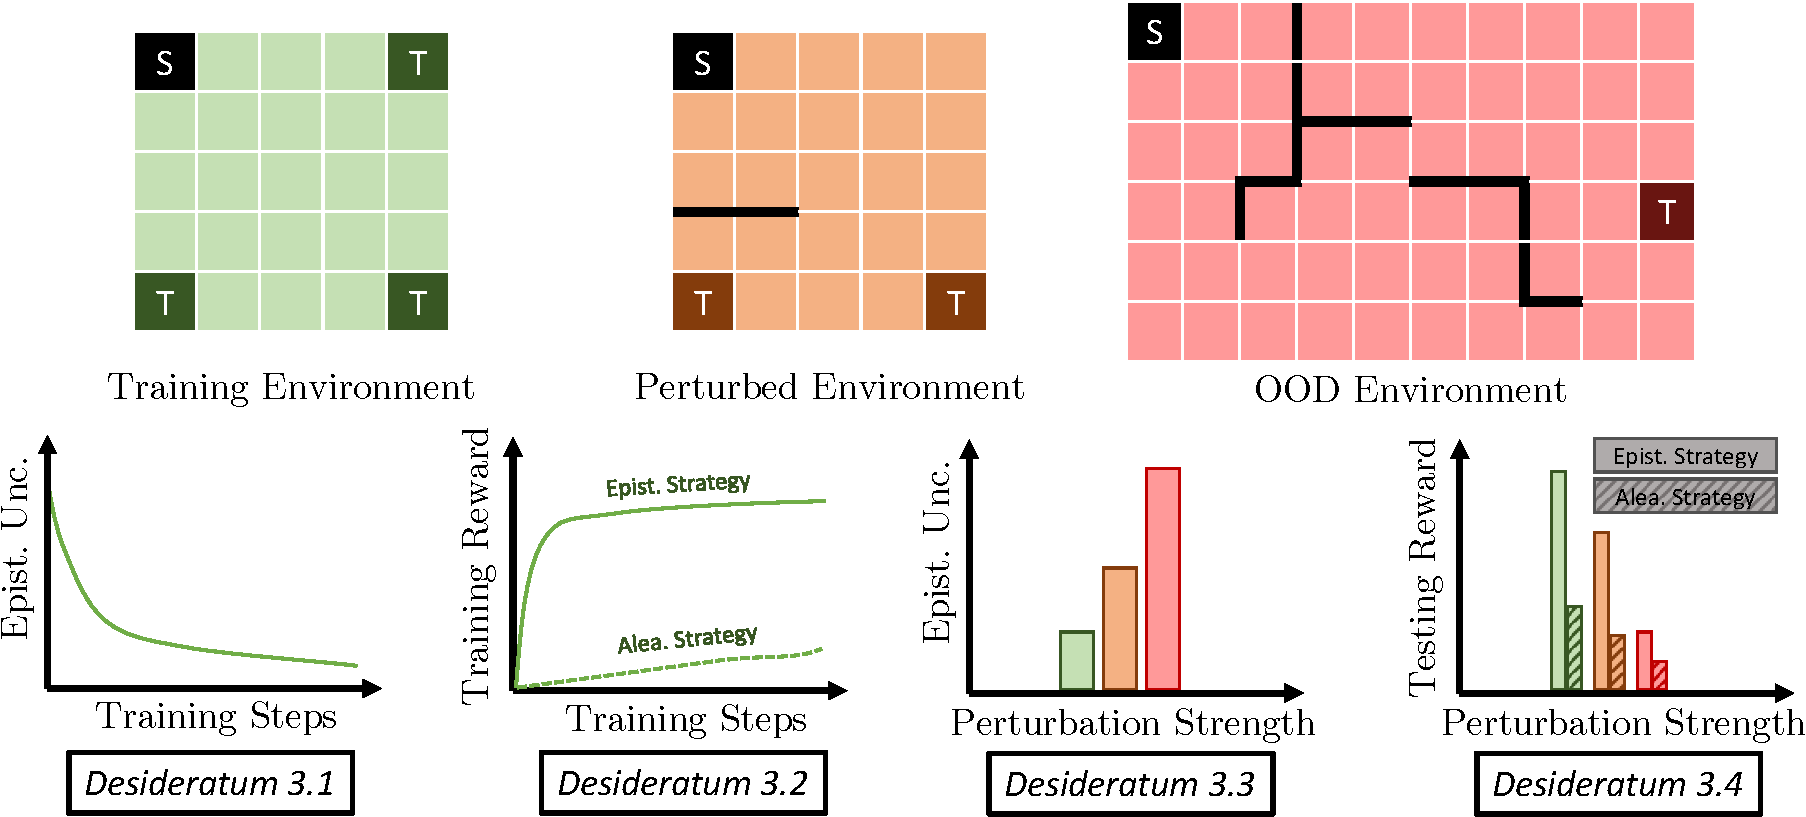
\includegraphics[width=.99\linewidth]{sections/011_icml2022/resources/diagram-cropped_2.pdf}
    \caption{Overview of our proposed desiderata for uncertainty in RL (See sec.~\ref{sec:desiderata_011}).}
    \label{fig:diagram}
\end{figure}

\looseness=-1
The core motivation of our work is to disentangle the properties of aleatoric and epistemic uncertainty estimates in RL to build agents with reliable performance in real-world applications. This motivation is similar to supervised learning (SL) where previous works defined \emph{desiderata}, \emph{models}, and \emph{evaluation} methods for aleatoric and epistemic uncertainty \cite{uncertainty-deep-learning, review-uncertainty-dl, dataset-shift, robustness-uncertainty-dirichlet}. Important examples of models using a single or multiple forward passes for uncertainty estimation in SL are MC dropout \cite{dropout}, ensemble \cite{ensembles, hyper-ensembles, batch-ensembles}, deep kernel learning \cite{simple-baseline-uncertainty, due, duq, uceloss}, and evidential networks \cite{postnet, priornet, natpn, evidential-regression}. Further, empirical evaluation of uncertainty estimates in SL focuses \emph{only} on testing time with Out-Of-Distribution (OOD) detection and generalization or detection of shifts \citep{dataset-shift, shifts-dataset}. In contrast to SL, the RL setting is more complex since it cares about the performance of uncertainty estimates at \emph{both} training and testing time.

\looseness=-1
\paragraph{Our Contributions.} In this work, we propose a framework for aleatoric and epistemic uncertainty estimation in RL: \textbf{(Desiderata)} We explicitly define four desiderata for uncertainty estimation in RL at both \emph{training} and \emph{testing time} (See fig.~\ref{fig:diagram}). They cover the behavior of \emph{aleatoric} and \emph{epistemic} uncertainty estimates w.r.t. the sample efficiency in the training environment and, w.r.t. the generalization performance in different testing environments. \textbf{(Models)} We carefully combine a diverse set of uncertainty estimation methods in SL (i.e. MC dropout, ensemble, deep kernel learning, and evidential networks) with Deep Q-Networks (DQN) \cite{dqn}, an ubiquitous RL model that is not equipped with uncertainty estimate by default. These combinations require a \emph{minimal} modification to the training procedure of the RL agent. We discuss \emph{theoretical} evidence on the ability of these combinations to fulfill the uncertainty desiderata. \textbf{(Evaluation)} Finally, we also propose a \emph{practical} methodology to evaluate uncertainty in RL based on OOD environments and domain shifts.

\section{Related Work}
\label{sec:related_work_007}

In this section, we describe other work related to uncertainty estimation for supervised learning. We refer to \citet{uncertainty-survey} for a detailed survey on uncertainty estimation in deep learning. 

\textbf{Sampling-based methods.} A first family of models estimates uncertainty by aggregating statistics (e.g. mean and variance) from different samples of an implicit predictive distribution. Examples are ensemble \citep{bayesian-classifier-combination,ensembles, dynamic-bayesian-combination-classifiers,batch-ensembles,hyper-ensembles} and dropout \citep{dropout} models which provide high-quality uncertainty estimates \citep{dataset-shift} at the cost of an
expensive sampling phase at inference time. Moreover, ensembles usually require training multiple models. Further, Bayesian neural networks (BNN) \citep{bayesian-networks, scalable-laplace-bnn, simple-baseline-uncertainty} model the uncertainty on the weights and also require multiple samples to estimate the uncertainty on the final prediction. While recent BNNs have shown reasonably good performance \citep{rank-1-bnn,practical-bayesian,liberty-depth-bnn}, modelling the distribution on the weights suffers from pathological behavior thus limiting these approaches in practice \citep{expressiveness-bnn, practical-bnn, what-bnn-posterior}. In particular, \citet{what-bnn-posterior} uses an enormous computation budget by parallelizing the computation over 512 TPUv3  devices and running tens of thousands of training epochs to achieve a more exact Bayesian inference which is not suitable for practical applications. In contrast, \NatPNacro{} predicts uncertainty in \emph{a single forward pass} with a \emph{closed-form posterior distribution} over the target variable. \NatPNacro{} \emph{does not} model uncertainty on the weights.

\textbf{Sampling-free methods.} A second family of models is capable of estimating uncertainty in a single forward pass. The family of models parametrizing conjugate prior distributions is the main focus of this paper \citep{survey_evidential_uncertainty,evaluating_dbu,max_gap_id_ood,uncertainty-generative-classifier,multifaceted_uncertainty,graph_posterior, lightweight-prob-net}. Beyond this family of models, we differentiate between four other families of sampling-free models for uncertainty estimation. A first family aims at learning deep Gaussian processes with random features projections or learned inducing points \citep{uncertainty-distance-awareness, due, duq, uceloss}. A second family aims at learning deep energy-based models \citep{ood_ebm, jem_ebm}. Another family of models aims at propagating uncertainty across layers \citep{natural-parameter-network, sampling-free-variance-propagation, feed-forward-propagation, lightweight-prob-net, probabilistic-backprop-scalable-bnn}. They model uncertainty at the weight and/or activation levels and are generally constrained to specific transformations. In contrast, \NatPNacro{} only models the uncertainty on the predicted target variable and does not enforce any constraint on the encoder architecture. Further, some of the models propagating uncertainty already used the exponential family framework \citep{natural-parameter-network, deep-exponential-families}. However, while they parametrize exponential family distributions, \NatPNacro{} parametrizes the \emph{conjugate prior of the target exponential family distributions} which accounts for the epistemic uncertainty. Finally, while the family of calibration models aims at calibrating predictions \citep{accurate-uncertainties-deep-learning-regression, confidence-aware-learning, individual-calibration, distribution-calibration-regression, intra-order-preserving}, \NatPNacro{} aims at accurately modelling both aleatoric and epistemic uncertainty on in- and out-of-distribution data.

\section{Natural Posterior Network}
\label{sec:model_007}

At the very core of \NatPNacro{} stands the Bayesian update rule: $    \prior(\expparam \condition \mathcal{D}) \propto \prob(\mathcal{D} \condition \expparam) \times \prior(\expparam)$
%
%\begin{equation}\label{eq:general-bayesian-update}
%    \prior(\expparam \condition \mathcal{D}) \propto \prob(\mathcal{D} \condition \expparam) \times \prior(\expparam)
%\end{equation}
%
where $\prob(\mathcal{D} \condition \expparam)$ is the target distribution of the target data $\mathcal{D}$ given its parameter $\expparam$, and $\prior(\expparam )$ and $\prior(\expparam \condition \mathcal{D})$ are the prior and posterior distributions, respectively, over the target distribution parameters. The target distribution $\prob(\mathcal{D} \condition \expparam)$ could be any likelihood describing the observed target labels. The Bayesian update has three main advantages: \textbf{(1)} it introduces a prior belief which represents the safe default prediction if no data is observed, \textbf{(2)} it updates the prior prediction based on observed target labels, and \textbf{(3)} it assigns a confidence for the new target prediction given the aggregated evidence count of observed target labels. While \NatPNacro{} is capable to perform a Bayesian update for every possible input given the observed training data, we first recall the Bayesian background for a single exponential family distribution.

\begin{table*}[ht!]
	\vspace{-3mm}
	\centering
	\resizebox{.89\textwidth}{!}{%
\begin{tabular}{lccl}
\toprule
\multicolumn{1}{c}{Likelihood $\prob$} & \multicolumn{1}{c}{Conjugate Prior $\prior$} & \multicolumn{1}{c}{Parametrization Mapping $m$} & \multicolumn{1}{c}{Bayesian Loss (Eq.~\ref{eq:bayesian-loss})}\\
\midrule
\midrule
$\y \sim \DCat(\bm{p})$ & 
$\bm{p} \sim \DDir(\bm{\alpha})$ & 
\begin{tabular}{@{}l@{}}
$\priorparam=\bm{\alpha}/\evidence$ \\
$\evidence=\sum_\iclass \alpha_\iclass$
\end{tabular} &
\begin{tabular}{@{}l@{}}
    \textbf{(i)} $= \psi(\alpha_{\y*}\dataix) - \psi(\alpha_0\dataix)$ \\
    \textbf{(ii)} $= \log B(\bm{\alpha}\dataix) + (\alpha_0\dataix - \nclass) \psi(\alpha_0\dataix) - \sum_\iclass (\alpha_\iclass\dataix - 1) \psi(\alpha_\iclass\dataix)$
\end{tabular} \\
\midrule
$\y \sim \DNormal(\mu, \sigma)$ & 
$\mu, \sigma \sim \DNIG(\mu_0, \lambda, \alpha, \beta)$ & 
\begin{tabular}{@{}l@{}}
$\priorparam=\begin{pmatrix}\mu_0 \\ \mu_0^2 + \frac{2\beta}{\evidence} \end{pmatrix}$\\
$\evidence = \lambda= 2 \alpha$
\end{tabular} &
\begin{tabular}{@{}l@{}}
    \textbf{(i)} $= \frac{1}{2}\left(- \frac{\alpha}{\beta} (\y - \mu_0)^2 - \frac{1}{\lambda} + \psi(\alpha) - \log{\beta} - \log{2\pi}\right)$ \\
    \textbf{(ii)} $= \frac{1}{2} + \log\left((2\pi)^{\frac{1}{2}}\beta^{\frac{3}{2}}\Gamma(\alpha)\right) - \frac{1}{2} \log{\lambda} + \alpha - (\alpha+\frac{3}{2})\psi(\alpha)$
\end{tabular}\\
\midrule
$\y \sim \DPoi(\lambda)$ &
$\lambda \sim \DGamma(\alpha, \beta)$ &
\begin{tabular}{@{}l@{}}
$\chi=\alpha/\evidence$ \\
$\evidence=\beta$
\end{tabular} &
\begin{tabular}{@{}l@{}}
    \textbf{(i)} $= (\psi(\alpha) - \log{\beta}) \y - \frac{\alpha}{\beta} - \sum_{k=1}^{\y} \log k$ \\
    \textbf{(ii)} $= \alpha + \log{\Gamma(\alpha)} - \log{\beta} + (1 - \alpha) \psi(\alpha)$
\end{tabular}\\
\bottomrule
\end{tabular}}
	\caption{Examples of Exponential Family Distributions where $\psi(x)$ and $B(x)$ denote Digamma and Beta function, respectively.}
	\label{tab:summary_exp_dist}
	\vspace{-3mm}
\end{table*}

\subsection{Exponential Family Distribution}
% \textbf{Exponential Family Distribution.} 
Distributions from the exponential family are very widely used and have favorable analytical properties. Indeed, \textbf{(1)} they cover a wide range of target variables like discrete, continuous, counts or spherical coordinates, and \textbf{(2)} they benefit from intuitive and generic formulae for their parameters, density functions and statistics which can often be evaluated in closed-form. Important examples of exponential family distributions are Normal, Categorical and Poisson distributions (see Tab.~\ref{tab:summary_exp_dist}). Formally, an exponential family distribution on a target variable $\y \in \real$ with \emph{natural parameters} $\expparam \in \real^\suffstatdim$ can be denoted as
%
\begin{equation}\label{eq:exponential-family}
    \prob(\y \condition \expparam) = h(\y) \exp\left(\expparam^T \bm{u}(\y) - A(\expparam)\right)
\end{equation}
%
where ${h: \real \rightarrow \real}$ is the \emph{carrier or base measure}, ${A: \real^\suffstatdim \rightarrow \real}$ the \emph{log-normalizer} and ${\bm{u}: \real \rightarrow \real^\suffstatdim}$ the \emph{sufficient statistics} \citep{bishop,exponential-entropy}. The entropy of an exponential family distribution can always be written as $\entropy[\prob] = A(\expparam) - \expparam^T \nabla_{\bm{\theta}}A(\expparam) - \expectation[\log{h(\y)}]$ \citep{exponential-entropy}.
An exponential family distribution always admits a conjugate prior, which often also is a member of the exponential family:
%
\begin{equation}\label{eq:prior}
    \prior(\expparam \condition \priorparam, \evidence) = \eta(\priorparam, \evidence) \exp\left( \evidence \, \bm{\theta}^T\priorparam  - \evidence A(\expparam) \right)
\end{equation}
%
where $\eta(\priorparam, \evidence)$ is a normalization coefficient, $\priorparam \in \real^L$ are \emph{prior parameters} and $\evidence \in \real^+$ is the \emph{evidence}. Given a set of $\ndata$ target observations $\{\y^{(i)}\}_{i}^{\ndata}$, it is easy to compute a closed-form Bayesian update $\prior(\expparam \condition \priorparam^\text{post}, \evidence^\text{post}) \propto \prob(\{\y^{(i)}\}_{i}^{\ndata} \condition \expparam) \times \prior(\expparam \condition \chi^\text{prior}, n^\text{prior})$:
%
\begin{equation}\label{eq:posterior}
    \prior(\expparam \condition \priorparam^\text{post}, \evidence^\text{post}) \propto \exp\left( \evidence^\text{post} \expparam^T\priorparam^\text{post} - \evidence^\text{post} A(\expparam) \right)
\end{equation}
%
where $\priorparam^\text{post}=\frac{\evidence^\text{prior} \priorparam^\text{prior}+ \sum_{j}^\ndata{\bm{u}(\y^{(j)})}}{\evidence^\text{prior} + \ndata}$ and $\evidence^\text{post}=\evidence^\text{prior} + \ndata$. We see that $\priorparam^{\text{prior}}$ (resp. $\priorparam^{\text{post}}$) can be viewed as the average sufficient statistics of $\evidence^{\text{prior}}$ (resp. $\evidence^{\text{post}}$) fictitious samples \citep{bishop}. 
Further, the average sufficient statistic of fictitious samples is equal to the expected sufficient statistic of the conjugate distribution, i.e. $\priorparam = \expectation_{\prior(\priorparam, \evidence)}[\expparam]$ \citep{exponential-family-stats, conjugate-prior-exponential-family}. Thus, the parameter $\priorparam^\text{post}$ carries the inherent aleatoric uncertainty on the target distribution with natural parameters $\expparam$, while the evidence $\evidence^\text{post}$ aligns well with the epistemic uncertainty (i.e. a low evidence means few prior target observations). We stress that the natural conjugate prior parametrization $\priorparam, \evidence$ is often different from the ``well-known'' parametrization $\bm{\kappa}$ used by standard coding libraries. By definition, a bijective mapping $m(\bm{\kappa}) = (\priorparam, \evidence)$ from the natural parametrization to the commonly used parametrization always exists (see examples in Tab.~\ref{tab:summary_exp_dist}). Finally, exponential family distributions always admit a closed-form posterior predictive distribution \citep{bayesian-data-analysis}.

\subsection{Input-Dependent Bayesian Update for Exponential Family Distributions}
%\textbf{Input-Dependent Bayesian Update for Exponential Family Distributions.} 
We propose to leverage the power of exponential family distributions for the more complex task when the prediction $\y\dataix$  depends on the input $\x\dataix$. Hence, \NatPNacro{} extends the Bayesian treatment of a single exponential family distribution prediction by predicting an individual posterior update per input. We distinguish between the chosen prior parameters $\priorparam^\text{prior}$, $\evidence^\text{prior}$ shared among samples, and the additional predicted parameters $\priorparam\dataix$, $\evidence\dataix$ dependent on the input $\x\dataix$ leading to the updated posterior parameters:
%
\begin{equation}\label{eq:parameter-update}
    \priorparam^{\text{post},(\idata)} = \frac{\evidence^\text{prior}\priorparam^\text{prior} + \evidence\dataix \priorparam\dataix}{\evidence^\text{prior} + \evidence\dataix}, \hspace{5mm}
    \evidence^{\text{post},(\idata)} = \evidence^\text{prior} + \evidence\dataix
\end{equation}
%
Equivalently, \NatPNacro{} may be interpreted as predicting a set of $\evidence\dataix$ pseudo observations $\{\y^{(j)}\}_{j}\dataix$ such that their aggregated sufficient statistics satisfy \smash{$\sum_{j}^{\evidence\dataix} \y^{(j)} = \evidence\dataix \priorparam\dataix$}, and perform the respective Bayesian update.
%
% \begin{equation}\label{eq:bayesian-update}
%     \begin{aligned}
% \prior(\expparam \condition \{\y^{(j)}\}_{j}\dataix) \propto \prob(\{\y^{(j)}\}_{j}\dataix \condition \expparam) \times \prior(\expparam)
%     \end{aligned}
% \end{equation}
%
This Bayesian update works for \emph{any} choice of exponential family distributions as long as parameters are mapped to their standard form (see Tab.~\ref{tab:summary_exp_dist}). According to the \emph{principle of maximum entropy} \citep{maximum-entropy-principle}, a practical choice for the prior is to enforce high entropy for the prior distribution which is usually considered less informative. It is typically achieved when the prior pseudo-count $\evidence^\text{prior}$ is small and the prior parameter $\priorparam^\text{prior}$ shows a high aleatoric uncertainty.

\begin{figure*}[t]
    \centering
    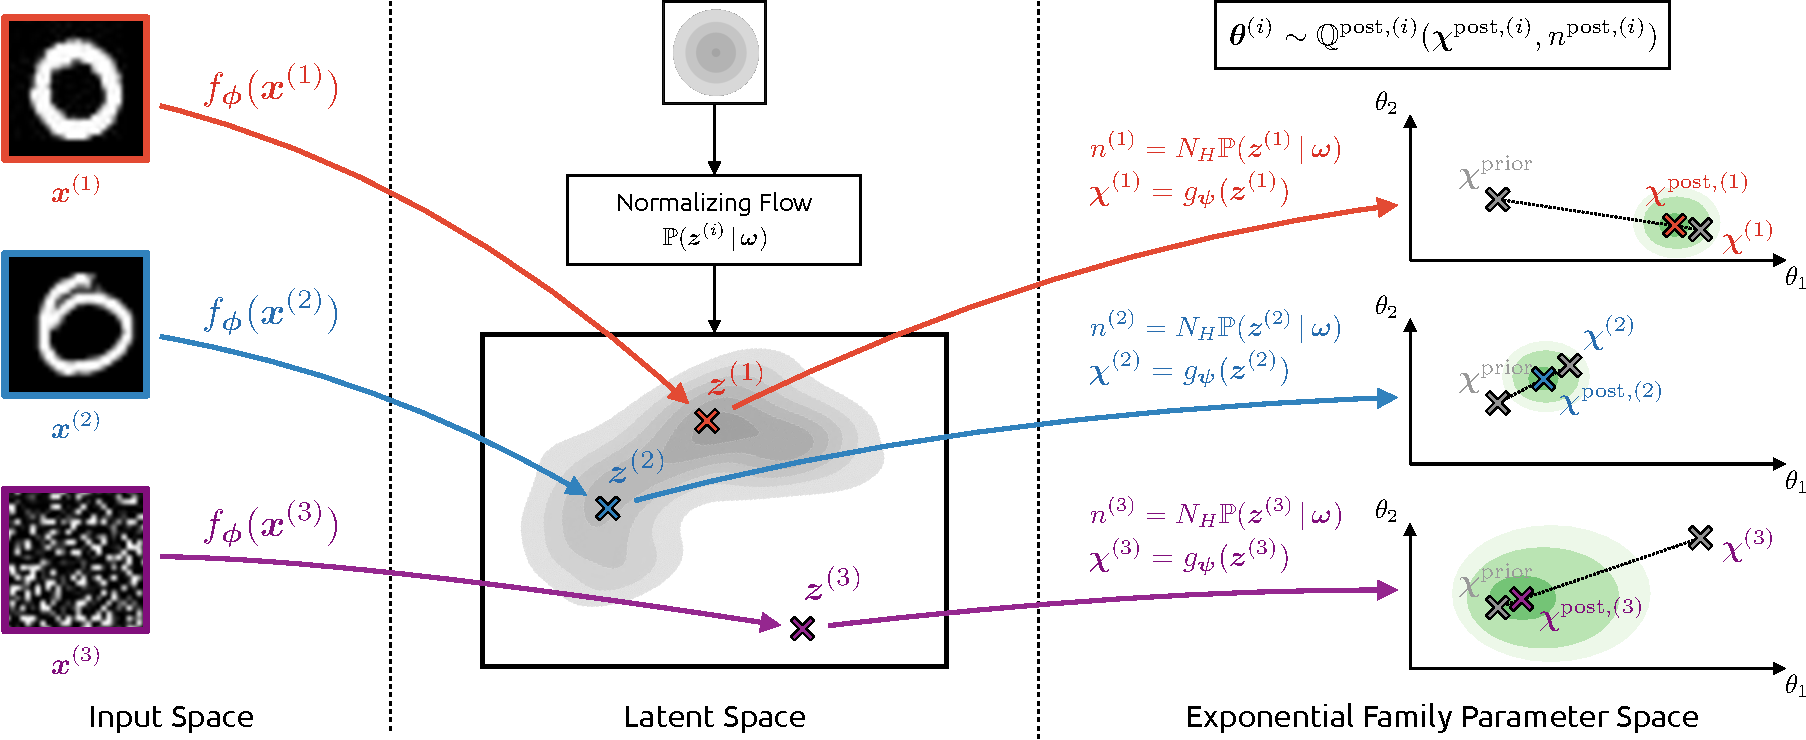
\includegraphics[width=.85\linewidth]{sections/007_iclr2022/resources/npn-crop.pdf}
    \caption{Overview of \NatPN{}. Inputs $\bm{x}^{(i)}$ are first mapped to a low-dimensional latent representation $\bm{z}^{(i)}$ by the encoder $f_{\bm{\phi}}$. From $\bm{z}^{(i)}$, the decoder $g_{\bm{\psi}}$ derives the parameter update $\bm{\chi}^{(i)}$ while a normalizing flow $\mathbb{P}_{\bm{\omega}}$ yields the evidence update $n^{(i)}$. Posterior parameters are obtained from a weighted combination of prior and update parameters according to $n^{\text{post},(i)}$.}
    \label{fig:npn}
    % \vspace{-1mm}
\end{figure*}

Hence, \NatPNacro{} proposes a generic way to perform the input-dependent Bayesian update $\priorparam\dataix$, $\evidence\dataix$ for \emph{any} exponential family distribution in three steps (see Fig.~\ref{fig:npn}): \textbf{(1)} An encoder $f_{\bm{\phi}}$ maps the input $\x\dataix$ onto a low-dimensional latent vector $\z\dataix = f_{\phi}(\x\dataix) \in \real^H$ representing useful features for the prediction task (see left Fig.\ref{fig:npn}). Note that the architecture of the encoder can be arbitrarily complex. Then, \textbf{(2)} the latent representation $\z\dataix$ is used in two different ways to predict the parameter update $\priorparam\dataix$ and the evidence update $\evidence\dataix$ (see center Fig.\ref{fig:npn}). On the one hand, a linear decoder $g_{\bm{\psi}}$ is trained to output the parameter update $\priorparam\dataix = g_{\bm{\psi}}(\z\dataix) \in \real^L$ accounting for the aleatoric uncertainty. On the other hand, a single normalized density is trained to output the evidence update $\evidence\dataix = N_H\prob(\z\dataix \condition \bm{\omega})$ accounting for the epistemic uncertainty. The intuition is that increasing the evidence on training data during training forces the evidence everywhere else (incl. far from training data) to decrease thanks to the density normalization constraint. The constant $N_H$ is a certainty budget distributed by the normalized density $\prob(\z\dataix \condition \bm{\omega})$ over the latent representations $\z\dataix$ i.e. $N_H = \int N_H \prob(\z\dataix \condition \bm{\omega}) d\z\dataix = \int \evidence\dataix d\z\dataix$. In practice, we observed that scaling the certainty budget w.r.t. the latent dimension $H$ helped the density to cover larger volumes in higher dimension (see app.). Finally, \textbf{(3)} \NatPNacro{} computes the posterior parameters $\priorparam^{\text{post}, (\idata)}$ and $\evidence^{\text{post}, (\idata)}$ which can be viewed respectively as the mean and concentration of the posterior distribution (see right Fig.\ref{fig:npn}). Note that the posterior parameter $\priorparam^{\text{post}, (\idata)}$ is a simple weighted average of the prior parameter $\priorparam^\text{prior}$ and the update parameter $\priorparam\dataix$ as shown by Eq.~\ref{eq:parameter-update}.

\NatPNacro{} extends PostNet \citep{postnet} which also performs an input-dependent Bayesian update with density estimation. Yet, it has three crucial differences which lead to major practical improvements. First, the new exponential family framework is significantly more flexible and is not restricted to classification. Second, the Dirichlet $\bm{\alpha}$ parameter computation is different: \NatPNacro{} computes the $\priorparam$ parameters -- which can be viewed as standard softmax output -- and the $\evidence$ evidence separately (i.e. $\bm{\alpha} = \evidence \priorparam$) while PostNet computes one evidence pseudo-count per class. Third, \NatPNacro{} is computationally more efficient. It requires a single density while PostNet requires $\nclass$ densities.

\subsection{ID and OOD Uncertainty Estimates}
%\textbf{ID and OOD Uncertainty Estimates.} 
\NatPNacro{} intuitively leads to reasonable uncertainty estimation for the two limit cases of strong in-distribution (ID) and out-of-distribution (OOD) inputs (see red and purple samples in Fig.~\ref{fig:npn}). For very likely \emph{in-distribution} data (i.e. $\prob(\z\dataix \condition \bm{\omega}) \rightarrow \infty$), the posterior parameter overrules the prior (i.e. $\priorparam^{\text{post}, (\idata)} \rightarrow \priorparam\dataix$). Conversely, for very unlikely \emph{out-of-distribution} data (i.e. $\prob(\z\dataix \condition \bm{\omega}) \rightarrow 0$), the prior parameter takes over in the posterior update (i.e. $\priorparam^{\text{post}, (\idata)} \rightarrow \priorparam^\text{prior}$). Hence, the choice of the prior parameter should reflect the default prediction when the model lacks knowledge. We formally show under mild assumptions on the encoder that \NatPNacro{} predicts very low additional evidence ($\evidence\dataix \approx 0$) for (almost) any input $\x\dataix$ far away from the training data (i.e. $||\x\dataix|| \rightarrow + \infty$), thus recovering prior predictions (i.e. $\priorparam^{\text{post}, (\idata)} \approx \priorparam^\text{prior}$) (see proof in app.).
\begin{theorem}
\label{thm:oodom-guarantee}
Let a \NatPNacro{} model be parametrized with a (deep) encoder $f_{\phi}$ with ReLU activations, a decoder $g_{\psi}$ and the density $\prob(\z \condition \bm{\omega})$. Let $f_{\phi}(\x)= V^{(l)}\x + a^{(l)}$ be the piecewise affine representation of the ReLU network $f_{\phi}$ on the finite number of affine regions $Q^{(l)}$ \citep{understanding-nn-relu}. Suppose that $V^{(l)}$ have independent rows and the density function $\prob(\z \condition \bm{\omega})$ has bounded derivatives, then for almost any $\x$ we have \smash{$\prob(f_{\phi}(\delta \cdot \x) \condition \bm{\omega}) \underset{\delta \rightarrow \infty}{\rightarrow} 0$}. i.e the evidence becomes small far from training data.
\end{theorem}
This theorem only requires that the density avoids very unlikely pathological behavior with unbounded derivatives \citep{limit-existence-infinity}. A slightly weaker conclusion holds using the notion of limit in density if the density function does not have bounded derivatives \citep{integrable-infinity}. Finally, the independent rows condition is realistic for trained networks with no constant output \citep{overconfident-relu}. It advantageously leads \NatPNacro{} to consistent uncertainty estimation contrary to standard ReLU networks which are overconfident far from training data \citep{overconfident-relu}.

\subsection{Bayesian \NatPNacro{} Ensemble} 
%\textbf{Bayesian \NatPNacro{} Ensemble.} 
Interestingly, it is natural to extend the Bayesian treatment of a single \NatPNacro{} to an ensemble of \NatPNacro{} models (NatPE). An ensemble of $m$ \NatPNacro{} models is intuitively equivalent to performing $m$ successive Bayesian updates using each \NatPNacro{} member separately. More formally, given an input $\x\dataix$ and an ensemble of $m$ jointly trained \NatPNacro{} models, the Bayesian update for the posterior distribution becomes ${\priorparam^{\text{post}, (\idata)} = \frac{\evidence^\text{prior}\priorparam^\text{prior} + \sum_k^{m} \evidence_k\dataix \priorparam_k\dataix}{\evidence^\text{prior} + \sum_k^{m} \evidence_k\dataix}}$ and ${\evidence^{\text{post}, (\idata)} = \evidence^\text{prior} + \sum_k^{m} \evidence_k\dataix}$. %which is equivalent to having observed $m$ sets of \smash{$\evidence_k\dataix$} pseudo observations. %$\{\y_k^{(j)}\}_{j}\dataix$ such that $\sum_{j}^{\evidence_m\dataix} \y^{(j)} = \priorparam_k\dataix$. 
Note that the standard Bayesian averaging which is used in many ensembling methods \citep{bayesian-ensemble-learning,ensembles,batch-ensembles,hyper-ensembles} is different from this Bayesian combination. While Bayesian averaging assume that only one model is correct, the Bayesian combination of \NatPNacro{} allows \emph{more} or \emph{none} of the models to be ``expert'' for some input  \citep{bayesian-averaging-to-combination}. For example, an input $\x\dataix$ unfamiliar to every model $m$ (i.e. $\evidence_m\dataix \approx 0$) would recover the prior default prediction $\priorparam^\text{prior}, \evidence^\text{prior}$. Existing models already had similar properties for Bayesian combination of classifiers \citep{bayesian-classifier-combination, dynamic-bayesian-combination-classifiers}.

\subsection{Optimization}
\label{sec:optimization}

The choice of the optimization procedure is of primary importance in order to obtain both high-quality target predictions and uncertainty estimates regardless of the task.

\paragraph{Bayesian Loss.} We follow \cite{postnet} and aim at minimizing the Bayesian formulation:
%
\begin{equation}\label{eq:bayesian-loss}
    \mathcal{L}\dataix = - \underbrace{\expectation_{\expparam\dataix \sim \prior^{\text{post},(\idata)}}[\log \prob(\y\dataix\condition \expparam \dataix)]}_\text{(i)} - \underbrace{\entropy[\prior^{\text{post},(\idata)}]}_\text{(ii)}
\end{equation}
%
where $\entropy[\prior^{\text{post},(\idata)}]$ denotes the entropy of the predicted posterior distribution $\prior^{\text{post},(\idata)}$. Similarly to the ELBO loss, this loss is guaranteed to be optimal when the predicted posterior distribution is close to the true posterior distribution $\prior^*(\expparam \condition \x\dataix)$ i.e. $\prior^{\text{post},(\idata)} \approx \prior^*(\expparam \condition \x\dataix)$ \citep{update-belief-propagation, PAC-bayesian_estimator, opt-info-processing_bayes}. However, this loss is generally \emph{not} equal to the ELBO loss especially for real valued targets i.e. $y \in \real$ (see app.). The term \textbf{(i)} is the expected likelihood under the predicted posterior distribution. It can be viewed as the Uncertain Cross Entropy (UCE) loss \citep{uceloss} which is known to reduce uncertainty on observed data. The term \textbf{(ii)} is an entropy regularizer acting as a prior which favors uninformative distributions $\prior^{\text{post},(\idata)}$ with high entropy. In our case, we assume the likelihood $\prob(\y\dataix\condition\expparam\dataix)$ and the posterior $\prior^{\text{post},(\idata)}$ to be members of the exponential family. We take advantage of the convenient computations for such distributions and derive a more explicit formula for the Bayesian formulation \eqref{eq:bayesian-loss} (see derivation in the appendix):
%
\begin{equation}\label{eq:nll-entropy}
    \begin{aligned}
    \mathcal{L}_\lambda\dataix &\propto \expectation[\expparam]^T \bm{u}(y\dataix) - \expectation[A(\bm{\expparam})] - \lambda\entropy[\prior^{\text{post},(\idata)}]
    \end{aligned}
\end{equation}
%
where $\lambda$ is an additional regularization weight tuned with a grid search. Note that the term $\expectation[\expparam]^T \bm{u}(y\dataix) $ favors a good alignment of the expected sufficient statistic $\expectation[\expparam] = \priorparam$ with the observed sufficient statistic $\bm{u}(y\dataix)$. In practice, all terms can be computed efficiently in closed form for most exponential family distributions (see examples in Tab.~\ref{tab:summary_exp_dist}). In particular, simplifications are possible when the conjugate prior distribution is also in an exponential family which is often the case. Ultimately Eq.~\eqref{eq:nll-entropy} applies to \emph{any} exponential family distribution unlike \cite{postnet}.

\textbf{Optimization Scheme.} \NatPNacro{} is fully differentiable using the closed-form Bayesian loss. Thus, we train the encoder $f_{\bm{\phi}}$, the parameter decoder $g_{\bm{\psi}}$ and the normalizing flow $\prob(\z\dataix \condition \bm{\omega})$ w.r.t. parameters $\bm{\phi}, \bm{\psi}, \bm{\omega}$ jointly. Further, we observed that ``warm-up training'' \citep{warm-start} and ``fine-tuning'' \citep{fine-tuning-continuous} of the density helped to improve uncertainty estimation for more complex flows and datasets. Thus, we train the normalizing flow density to maximize the likelihood of the latent representations before and after the joint optimization while keeping all other parameters fixed.

\subsection{Model Limitations} \label{sec:limitations}

\paragraph{Task-Specific OOD.} Previous works show that density estimation is unsuitable for acting on the raw image input \citep{anomaly-detection,deep-generative,typicality_OOD_generative} or on a non-carefully transformed space \citep{perfect-density-no-ood-guarantee}. To circumvent this issue, \NatPNacro{} does not perform OOD detection directly on the input but rather fits a normalizing flow on a learned space. In particular, the latent space is \textbf{(1)} low-dimensional, \textbf{(2)} task-specific and \textbf{(3)} encodes meaningful semantic features. Similarly, \cite{postnet, why-nf-fail-ood, density-states-ood, contrastive-ood} already improved OOD detection of density-based methods by leveraging a task-induced bias or low-dimensional statistics. In the case of \NatPNacro{}, the low-dimensional latent space has to contain relevant features to linearly predict the sufficient statistics required for the task. For example, \NatPNacro{} aims at a linearly separable latent space for classification. The downside is that \NatPNacro{} is capable of detecting OOD samples only with respect to the considered task and requires labeled examples during training. As an example, \NatPNacro{} likely fails to detect a change of image color if the task aims at classifying object shapes and the latent space has no notion of color. Hence, we underline that \NatPNacro{} comes with a task-dependent OOD definition, which is a reasonable choice in practice.

\paragraph{Model-Task Mismatch.} Second, we emphasize that the uncertainty estimation quality of \NatPNacro{} for (close to) ID data depends on the convergence of the model, the encoder architecture (e.g. MLP, Conv., DenseDepth \citep{dense-depth}) and the target distribution (e.g. Poisson, Normal distributions) choice which should match the task needs. However, we show \emph{empirically} that \NatPNacro{} provides high quality uncertainty estimates in practice on a wide range of tasks. Further, we show \emph{theoretically} that \NatPNacro{} leads to uncertain prediction far away from training data for \emph{any} exponential family target distributions. In comparison, \cite{provable-uncertainty} showed akin guarantees for classification only.
\section{Experiments}
\label{sec:experiments_007}

In this section, we compare \NatPNacro{} to existing methods on extensive experiments including three different tasks: classification, regression and count prediction. For each task type, we evaluate the prediction quality based on target error and uncertainty metrics. These various set-ups aim to highlight the versatility of \NatPNacro{}. In particular, \NatPNacro{} is the only model that adapts to all tasks and achieves high performances for all metrics without requiring multiple forward passes.

\begin{table*}[ht]
    \centering
    % \vspace{-1mm}
   % \scriptsize
   \caption{Classification results on Sensorless Drive with Categorical target distribution. Best scores among all single-pass models are in bold. Best scores among all models are starred.}
    \label{tab:sensorless-drive}
    % \vspace{-3mm}
    \resizebox{0.8 \textwidth}{!}{
    \begin{tabular}{lcccccc}
        \toprule
        & \textbf{Accuracy} & \textbf{Brier} & \textbf{9/10 Alea.} & \textbf{9/10 Epist.} & \textbf{OODom Alea.} & \textbf{OODom Epist.} \\
        \midrule
        \textbf{Dropout} & 98.62 $\pm$ 0.11 & 3.79 $\pm$ 0.29 & 30.20 $\pm$ 0.85 & 32.57 $\pm$ 1.45 & 27.03 $\pm$ 0.51 & 95.30 $\pm$ 1.66 \\
        \textbf{Ensemble} & 98.83 $\pm$ 0.17 & 3.00 $\pm$ 0.54 & 30.79 $\pm$ 0.74 & 32.61 $\pm$ 1.06 & 27.16 $\pm$ 0.59 & 99.97 $\pm$ 0.01 \\
        \textbf{NatPE} & *99.66 $\pm$ 0.03 & *0.68 $\pm$ 0.05 & 77.05 $\pm$ 1.93 & 83.73 $\pm$ 1.89 & 99.99 $\pm$ 0.00 & *100.00 $\pm$ 0.00 \\
        \midrule
        \textbf{R-PriorNet} & 98.85 $\pm$ 0.25 & 2.01 $\pm$ 0.47 & 40.13 $\pm$ 2.99 & 30.07 $\pm$ 0.81 & \textbf{*100.00 $\pm$ 0.00} & 23.59 $\pm$ 0.00 \\
        \textbf{EnD$^2$} & 93.95 $\pm$ 2.35 & 28.09 $\pm$ 6.40 & 26.35 $\pm$ 0.60 & 24.85 $\pm$ 0.43 & 84.43 $\pm$ 15.21 & 23.58 $\pm$ 0.00 \\
        \textbf{PostNet} & \textbf{99.64 $\pm$ 0.02} & \textbf{0.75 $\pm$ 0.08} & 80.60 $\pm$ 1.68 & \textbf{*92.57 $\pm$ 1.41} & \textbf{*100.00 $\pm$ 0.00} & \textbf{*100.00 $\pm$ 0.00} \\
        \textbf{\NatPNacro{}} & 99.61 $\pm$ 0.05 & 1.04 $\pm$ 0.29 & \textbf{*81.43 $\pm$ 1.89} & 79.54 $\pm$ 2.62 & 99.98 $\pm$ 0.00 & \textbf{*100.00 $\pm$ 0.00} \\
        \bottomrule
    \end{tabular}
    }
            % \vspace{-0mm}
\end{table*}

%\begin{table*}[ht]
%    \centering
%    \scriptsize
%    \resizebox{1.\textwidth}{!}{
%    \begin{tabular}{lcccccccc}
%        \toprule
%        & \textbf{Accuracy} & \textbf{Brier} & \textbf{K. Alea.} & \textbf{K. Epist.} & \textbf{F. Alea.} & \textbf{F. Epist.} & \textbf{OODom Alea.} & \textbf{OODom Epist.} \\
%        \midrule
%        \textbf{Dropout} & 99.45 $\pm$ 0.01 & 1.07 $\pm$ 0.05 & 98.27 $\pm$ 0.05 & 97.82 $\pm$ 0.08 & *99.40 $\pm$ 0.03 & 98.01 $\pm$ 0.14 & 43.86 $\pm$ 1.62 & 74.09 $\pm$ 0.92 \\
%        \textbf{Ensemble} & 99.46 $\pm$ 0.02 & 1.02 $\pm$ 0.02 & 98.39 $\pm$ 0.07 & 98.43 $\pm$ 0.05 & 99.33 $\pm$ 0.06 & 98.73 $\pm$ 0.08 & 40.98 $\pm$ 1.80 & 66.54 $\pm$ 0.58 \\
%        \textbf{NatPE} & *99.55 $\pm$ 0.01 & *0.84 $\pm$ 0.03 & 96.39 $\pm$ 0.73 & *99.61 $\pm$ 0.02 & 97.49 $\pm$ 0.85 & *99.70 $\pm$ 0.04 & *100.00 $\pm$ 0.00 & *100.00 $\pm$ 0.00 \\
%        \midrule
%        \textbf{R-PriorNet} & 99.35 $\pm$ 0.04 & \textbf{0.97 $\pm$ 0.03} & \textbf{*99.33 $\pm$ 0.18} & 99.28 $\pm$ 0.25 & \textcolor{gray}{100.00 $\pm$ 0.00} & \textcolor{gray}{100.00 $\pm$ 0.00} & 97.48 $\pm$ 0.66 & 31.03 $\pm$ 0.13 \\
%        \textbf{EnD$^2$} & 99.24 $\pm$ 0.05 & 6.19 $\pm$ 0.13 & 98.36 $\pm$ 0.15 & 98.76 $\pm$ 0.13 & \textbf{99.25 $\pm$ 0.16} & 99.35 $\pm$ 0.14 & 48.09 $\pm$ 1.38 & 31.60 $\pm$ 0.39 \\
%        \textbf{PostNet} & 99.36 $\pm$ 0.02 & 1.33 $\pm$ 0.04 & 98.88 $\pm$ 0.05 & 98.79 $\pm$ 0.07 & 98.89 $\pm$ 0.23 & 98.85 $\pm$ 0.23 & \textbf{*100.00 $\pm$ 0.00} & \textbf{*100.00 $\pm$ 0.00} \\
%        \textbf{\NatPNacro{}} & \textbf{99.47 $\pm$ 0.02} & 1.09 $\pm$ 0.03 & 99.20 $\pm$ 0.20 & \textbf{99.39 $\pm$ 0.08} & 99.16 $\pm$ 0.28 & \textbf{99.54 $\pm$ 0.09} & 99.99 $\pm$ 0.01 & \textbf{*100.00 $\pm$ 0.00} \\
%        \bottomrule
%    \end{tabular}
%    }
%    \caption{Results on MNIST (classification with Categorical target distribution). Best scores among all single-pass models are in bold. Best scores among all models are starred. Gray numbers indicate that R-PriorNet has seen samples from the FMNIST dataset during training.}
%    \label{tab:mnist}
            %\vspace{-.3cm}
%\end{table*}

%\begin{table*}[ht]
% \centering
% \scriptsize
% \resizebox{\textwidth}{!}{
% \begin{tabular}{lcccccccc}
%     \toprule
%     & \textbf{Accuracy} & \textbf{Brier} & \textbf{M. Alea.} & \textbf{M. Epist.} & \textbf{K. Alea.} & \textbf{K. Epist.} & \textbf{OODom Alea.} & \textbf{OODom Epist.} \\
%     \midrule
%     \textbf{Dropout} & 92.44 $\pm$ 0.17 & 13.89 $\pm$ 0.31 & 60.75 $\pm$ 1.41 & 75.85 $\pm$ 1.73 & 76.57 $\pm$ 1.30 & 92.48 $\pm$ 0.46 & 39.97 $\pm$ 0.69 & 90.90 $\pm$ 1.74 \\
%     \textbf{Ensemble} & 92.64 $\pm$ 0.10 & 13.63 $\pm$ 0.25 & 77.14 $\pm$ 1.49 & 90.78 $\pm$ 0.75 & 86.20 $\pm$ 0.76 & 95.16 $\pm$ 0.35 & 37.30 $\pm$ 0.83 & 82.93 $\pm$ 0.96 \\
%     \textbf{NatPE} & *92.89 $\pm$ 0.06 & 14.44 $\pm$ 0.06 & 82.56 $\pm$ 0.33 & 96.38 $\pm$ 0.29 & 92.12 $\pm$ 0.17 & *98.79 $\pm$ 0.09 & *100.00 $\pm$ 0.00 & *100.00 $\pm$ 0.00 \\
%     \midrule
%     \textbf{R-PriorNet} & 91.53 $\pm$ 0.10 & \textbf{*12.21 $\pm$ 0.20} & \textbf{*98.83 $\pm$ 0.49} & \textbf{*99.54 $\pm$ 0.18} & \textcolor{gray}{99.96 $\pm$ 0.02} & \textcolor{gray}{99.99 $\pm$ 0.00} & 72.23 $\pm$ 6.32 & 48.84 $\pm$ 6.09 \\
%     \textbf{EnD$^2$} & \textbf{91.84 $\pm$ 0.03} & 29.23 $\pm$ 0.79 & 79.32 $\pm$ 1.39 & 91.61 $\pm$ 1.04 & 91.99 $\pm$ 0.06 & 98.36 $\pm$ 0.20 & 43.70 $\pm$ 3.37 & 36.73 $\pm$ 3.74 \\
%     \textbf{PostNet} & 91.04 $\pm$ 0.10 & 16.11 $\pm$ 0.30 & 90.56 $\pm$ 1.25 & 92.10 $\pm$ 1.77 & \textbf{*96.65 $\pm$ 0.33} & 97.06 $\pm$ 0.42 & \textbf{*100.00 $\pm$ 0.00} & \textbf{*100.00 $\pm$ 0.00} \\
%     \textbf{\NatPNacro{}} & 91.65 $\pm$ 0.14 & 14.88 $\pm$ 0.30 & 81.12 $\pm$ 2.77 & 96.51 $\pm$ 0.81 & 93.03 $\pm$ 1.00 & \textbf{98.38 $\pm$ 0.23} & 99.99 $\pm$ 0.01 & \textbf{*100.00 $\pm$ 0.00} \\
%     \bottomrule
% \end{tabular}
% }
% \caption{Results on FMNIST (classification with Categorical target distribution). Best scores among all single-pass models are in bold. Best scores among all models are starred. Gray numbers indicate that R-PriorNet has seen samples from the KMNIST dataset during training.}
% \label{tab:fmnist}
%\end{table*}

\begin{table*}[ht]
    \centering
    	% \vspace{-4mm}
    %\scriptsize
    \caption{Classification results on CIFAR-10 with Categorical target distribution. Best scores among all single-pass models are in bold. Best scores among all models are starred. Gray numbers indicate that R-PriorNet has seen samples from the SVHN dataset during training.}
    % \vspace{-3mm}
    \resizebox{.9\textwidth}{!}{
    \begin{tabular}{lcccccccc}
        \toprule
        & \textbf{Accuracy} & \textbf{Brier} & \textbf{SVHN Alea.} & \textbf{SVHN Epist.} & \textbf{CelebA Alea.} & \textbf{CelebA Epist.} & \textbf{OODom Alea.} & \textbf{OODom Epist.} \\
        \midrule
        \textbf{Dropout} & 88.15 $\pm$ 0.20 & 19.59 $\pm$ 0.41 & 80.63 $\pm$ 1.59 & 73.09 $\pm$ 1.51 & 71.84 $\pm$ 4.28 & 71.04 $\pm$ 3.92 & 18.42 $\pm$ 1.11 & 49.69 $\pm$ 9.10 \\
        \textbf{Ensemble} & *89.95 $\pm$ 0.11 & 17.33 $\pm$ 0.17 & 85.26 $\pm$ 0.84 & 82.51 $\pm$ 0.63 & 76.20 $\pm$ 0.87 & 74.23 $\pm$ 0.78 & 25.30 $\pm$ 4.02 & 89.21 $\pm$ 7.55 \\
        \textbf{NatPE} & 89.21 $\pm$ 0.09 & 17.41 $\pm$ 0.12 & 85.66 $\pm$ 0.34 & *83.16 $\pm$ 0.67 & *78.95 $\pm$ 1.15 & *82.06 $\pm$ 1.30 & 87.27 $\pm$ 1.79 & *98.88 $\pm$ 0.26 \\
        \midrule
        \textbf{R-PriorNet} & \textbf{88.94 $\pm$ 0.23} & \textbf{*15.99 $\pm$ 0.32} & \textcolor{gray}{99.87 $\pm$ 0.02} & \textcolor{gray}{99.94 $\pm$ 0.01} & 67.74 $\pm$ 4.86 & 59.55 $\pm$ 7.90 & 42.21 $\pm$ 8.77 & 38.25 $\pm$ 9.82 \\
        \textbf{EnD$^2$} & 84.03 $\pm$ 0.25 & 40.84 $\pm$ 0.36 & \textbf{*86.47 $\pm$ 0.66} & \textbf{81.84 $\pm$ 0.92} & 75.54 $\pm$ 1.79 & 75.94 $\pm$ 1.82 & 42.19 $\pm$ 8.77 & 15.79 $\pm$ 0.27 \\
        %\textbf{SNGP} & 79.40 $\pm$ 0.96 & 38.76 $\pm$ 1.61 & 71.65 $\pm$ 0.89 & -- & 72.46 $\pm$ 2.23 & -- & 83.35 $\pm$ 5.93 & -- \\
        \textbf{PostNet} & 87.95 $\pm$ 0.20 & 20.19 $\pm$ 0.40 & 82.35 $\pm$ 0.68 & 79.24 $\pm$ 1.49 & 72.96 $\pm$ 2.33 & 75.84 $\pm$ 1.61 & 85.89 $\pm$ 4.10 & 92.30 $\pm$ 2.18 \\
        \textbf{\NatPNacro{}} & 87.90 $\pm$ 0.16 & 19.99 $\pm$ 0.46 & 82.29 $\pm$ 1.11 & 77.83 $\pm$ 1.22 & \textbf{76.01 $\pm$ 1.18} & \textbf{76.87 $\pm$ 3.38} & \textbf{*93.67 $\pm$ 3.03} & \textbf{94.90 $\pm$ 3.09} \\
        \bottomrule
    \end{tabular}
    }
    \label{tab:cifar10}
            % \vspace{-4mm}
\end{table*}

\begin{table*}[ht]
    \centering
    %\scriptsize
        \caption{Results on the Bike Sharing Dataset with Normal $\DNormal$ and Poison $\DPoi$ target distributions. Best scores among all single-pass models are in bold. Best scores among all models are starred.}
    \label{tab:bike-sharing}
    % \vspace{-3mm}
    \resizebox{0.9\textwidth}{!}{
    \begin{tabular}{lcccccc}
        \toprule
        & \textbf{RMSE} & \textbf{Calibration} & \textbf{Winter Epist.} & \textbf{Spring Epist.} & \textbf{Autumn Epist.} & \textbf{OODom Epist.} \\
        \midrule
        \textbf{Dropout-$\DNormal$} & 70.20 $\pm$ 1.30 & 6.05 $\pm$ 0.77 & 15.26 $\pm$ 0.51 & 13.66 $\pm$ 0.16 & 15.11 $\pm$ 0.46 & 99.99 $\pm$ 0.01 \\
        \textbf{Ensemble-$\DNormal$} & *48.02 $\pm$ 2.78 & 5.88 $\pm$ 1.00 & 42.46 $\pm$ 2.29 & 21.28 $\pm$ 0.38 & 21.97 $\pm$ 0.58 & *100.00 $\pm$ 0.00 \\
        \midrule
        \textbf{EvReg-$\DNormal$} & \textbf{49.58 $\pm$ 1.51} & 3.77 $\pm$ 0.81 & 17.19 $\pm$ 0.76 & 15.54 $\pm$ 0.65 & 14.75 $\pm$ 0.29 & 34.99 $\pm$ 17.02 \\
        \textbf{\NatPNacro{}-$\DNormal$} & 49.85 $\pm$ 1.38 & \textbf{*1.95 $\pm$ 0.34} & \textbf{*55.04 $\pm$ 6.81} & \textbf{*23.25 $\pm$ 1.20} & \textbf{*27.78 $\pm$ 2.47} & \textbf{*100.00 $\pm$ 0.00} \\
        \midrule
        \midrule
        \textbf{Dropout-$\DPoi$} & 66.57 $\pm$ 4.61 & 55.00 $\pm$ 0.22 & 16.02 $\pm$ 0.48 & 13.48 $\pm$ 0.38 & 18.09 $\pm$ 0.82 & \textbf{*100.00 $\pm$ 0.00} \\
        \textbf{Ensemble-$\DPoi$} & \textbf{*48.22 $\pm$ 2.06} & 55.31 $\pm$ 0.21 & 83.88 $\pm$ 1.22 & 34.21 $\pm$ 1.81 & 41.29 $\pm$ 3.23 & \textbf{*100.00 $\pm$ 0.00} \\
        \midrule
        \textbf{\NatPNacro{}-$\DPoi$} & 51.79 $\pm$ 0.78 & \textbf{*31.04 $\pm$ 1.81} & \textbf{*85.15 $\pm$ 3.61} & \textbf{*37.03 $\pm$ 2.35} & \textbf{*42.73 $\pm$ 4.38} & \textbf{*100.00 $\pm$ 0.00} \\
        \bottomrule
    \end{tabular}
    }
            % \vspace{-3mm}
\end{table*}

\begin{table*}[t]
    \centering
   % \scriptsize
   \caption{Regression results on models trained on different UCI datasets with Normal target distribution. The upper half displays models trained on Kin8nm, the lower half shows models trained on Concrete Compressive Strength.}
    \label{tab:uci}
    % \vspace{-3mm}
    \resizebox{1.\textwidth}{!}{
    \begin{tabular}{lcccccccc}
        \toprule
        & \textbf{RMSE} & \textbf{Calibration} & \textbf{Energy Alea.} & \textbf{Energy Epist.} & \textbf{Concrete Alea.} & \textbf{Concrete Epist.} & \textbf{Kin8nm Alea.} & \textbf{Kin8nm Epist.} \\
        \midrule
        \textbf{Dropout} & 0.09 $\pm$ 0.00 & 3.13 $\pm$ 0.43 & 90.18 $\pm$ 6.00 & 99.94 $\pm$ 0.06 & *100.00 $\pm$ 0.00 & *100.00 $\pm$ 0.00 & \multicolumn{2}{c}{\multirow{3}{*}{\textbf{in-distribution}}} \\
        \textbf{Ensemble} & *0.07 $\pm$ 0.00 & 2.69 $\pm$ 0.49 & *100.00 $\pm$ 0.00 & *100.00 $\pm$ 0.00 & *100.00 $\pm$ 0.00 & *100.00 $\pm$ 0.00 & & \\
        \textbf{NatPE} & 0.08 $\pm$ 0.00 & 5.49 $\pm$ 0.30 & *100.00 $\pm$ 0.00 & *100.00 $\pm$ 0.00 & *100.00 $\pm$ 0.00 & *100.00 $\pm$ 0.00 & & \\
        \midrule
        \textbf{EvReg} & 0.09 $\pm$ 0.00 & 3.74 $\pm$ 0.53 & 88.06 $\pm$ 11.94 & 88.06 $\pm$ 11.94 & \textbf{*100.00 $\pm$ 0.00} & 86.84 $\pm$ 13.16 & \multicolumn{2}{c}{\multirow{2}{*}{\textbf{in-distribution}}} \\
        \textbf{\NatPNacro{}} & \textbf{0.08 $\pm$ 0.00} & \textbf{*2.04 $\pm$ 0.45} & \textbf{*100.00 $\pm$ 0.00} & \textbf{*100.00 $\pm$ 0.00} & \textbf{*100.00 $\pm$ 0.00} & \textbf{*100.00 $\pm$ 0.00} & & \\
        \midrule
        \midrule
        \textbf{Dropout} & 5.67 $\pm$ 0.07 & *3.03 $\pm$ 0.40 & 9.33 $\pm$ 0.36 & 93.53 $\pm$ 2.41 & \multicolumn{2}{c}{\multirow{3}{*}{\textbf{in-distribution}}} & 1.09 $\pm$ 0.13 & 64.30 $\pm$ 7.14 \\
        \textbf{Ensemble} & 5.69 $\pm$ 0.20 & 3.81 $\pm$ 0.67 & 54.19 $\pm$ 18.93 & *100.00 $\pm$ 0.00 & & & 72.57 $\pm$ 19.32 & *100.00 $\pm$ 0.00 \\
        \textbf{NatPE} & *4.78 $\pm$ 0.20 & 5.58 $\pm$ 1.27 & *100.00 $\pm$ 0.00 & *100.00 $\pm$ 0.00 & & & *100.00 $\pm$ 0.00 & *100.00 $\pm$ 0.00 \\
        \midrule
        \textbf{EvReg} & 6.04 $\pm$ 0.18 & 7.36 $\pm$ 1.04 & 8.93 $\pm$ 0.02 & 51.39 $\pm$ 18.56 & \multicolumn{2}{c}{\multirow{2}{*}{\textbf{in-distribution}}} & 0.93 $\pm$ 0.00 & 34.44 $\pm$ 20.95 \\
        \textbf{\NatPNacro{}} & \textbf{5.83 $\pm$ 0.23} & \textbf{5.41 $\pm$ 1.33} & \textbf{*100.00 $\pm$ 0.00} & \textbf{*100.00 $\pm$ 0.00} & & & \textbf{*100.00 $\pm$ 0.00} & \textbf{*100.00 $\pm$ 0.00} \\
        \bottomrule
    \end{tabular}}
    % \vspace{-4mm}
\end{table*}

\begin{table*}[t]
    \centering
 %   \scriptsize
     \caption{Regression results on NYU Depth v2 with Normal target distribution. RMSE is in cm. OOD scores on LSUN are reported on the held-out classes `classrooms' (left) and `churches' (right).}
    \label{tab:nyu}
    \vspace{-0mm}
    \resizebox{1. \textwidth}{!}{
    \begin{tabular}{lcccccccccc}
        \toprule
        & \textbf{RMSE} & \textbf{Calibration} & \textbf{LSUN Alea.} & \textbf{LSUN Epist.} & \textbf{KITTI Alea.} & \textbf{KITTI Epist.} & \textbf{OODom Alea.} & \textbf{OODom Epist.} \\
        \midrule
        \textbf{Dropout} & 46.95 & 4.03 & *95.29 / 97.74 & 83.89 / 83.22 & 98.07 & 84.90 & 74.40 & *100.00 \\
        \midrule
        \textbf{EvReg} & \textbf{*28.88} & \textbf{*1.05} & 58.70 / 56.71 & 70.19 / 64.02 & 56.60 & 62.67 & 75.43 & 56.39 \\
        \textbf{\NatPNacro{}} & 29.72 & 1.14 & \textbf{94.13} / \textbf{*98.67} & \textbf{*89.08} / \textbf{*90.56} & \textbf{*98.93} & \textbf{*93.15} & \textbf{*100.00} & \textbf{*100.00} \\
        \bottomrule
    \end{tabular}}
    \vspace{-0mm}
\end{table*}

\subsection{Setup}

% \begin{wrapfigure}{r}{0.5\textwidth}
\begin{figure*}[t]
\vspace{-4mm}
	\centering
    \includegraphics[width=.8\linewidth]{sections/007_iclr2022/resources/corruptions-final-crop.pdf}
    \caption{Averaged accuracy and confidence under 15 dataset shifts on CIFAR-10 \citep{benchmarking-corruptions}. 
    On more severe perturbations (i.e. data further away from data distribution), \NatPNacro{} maintains a competitive accuracy while assigning higher epistemic uncertainty as desired. Baselines provide a slower relative confidence decay.
    }
    \label{fig:data-corruption}
\vspace{-4mm}
\end{figure*}
% \end{wrapfigure}

In our experiments, we change the encoder architecture of \NatPNacro{} to match the dataset needs. We perform a grid search over normalizing flows types (i.e. radial flows \citep{radialflow} and MAF \citep{made,maf}) and latent dimensions. We show further experiments on architecture, latent dimension, normalizing flow choices and certainty budget choice in the appendix. Furthermore, we use approximations of the log-Gamma $\log\Gamma(x)$ and the Digamma $\psi(x)$ functions for large input values to avoid unstable floating computations (see app.). As prior parameters, we set ${\bm{\chi}^\text{prior}=\bm{1}_{\nclass}/C}, {\evidence^\text{prior}=\nclass}$ for classification, ${\priorparam^\text{prior}=(0, 100)^T}, \evidence^\text{prior}=1$ for regression and $\chi^\text{prior}=1, \evidence^\text{prior}=1$ for count prediction enforcing high entropy for prior distributions.

\paragraph{Baselines.} We focus on recent models parametrizing prior distributions over the target distribution. For classification, we compare \NatPNacro{} to Reverse KL divergence Prior Networks (R-PriorNet) \citep{reverse-kl}, Ensemble Distribution Distillation (EnD$^2$) \citep{distribution-distillation} and Posterior Networks (PostNet) \citep{charpentier2020}. Note that Prior Networks require OOD training data --- we use an auxiliary dataset when available and Gaussian noise otherwise. For regression, we compare to Evidential Regression (EvReg) \citep{evidential-regression}. Beyond baselines parametrizing conjugate prior distributions, we also compare to dropout (Dropout) \citep{dropout} and ensemble (Ensemble) \citep{ensembles} models for all tasks. These sampling baselines require multiple forward passes for uncertainty estimation. 
Further details are given in the appendix.
%As suggested in \citep{dataset-shift}, we use $5$ samples for the two sampling baselines. Note that, unlike the other baselines or \NatPNacro{}, the sampling baselines require multiple forward passes for uncertainty estimation. 
%In all experiments, all models share the same backbone architecture (MLP, Conv. \citep{conv-net}, DenseDepth \citep{dense-depth}). We use early stopping and perform a grid search on the hyperparameters of all models including learning rate, dropout rate and regularizing factor when applicable. We report average results over $5$ initialization seeds with standard error of the mean (except for the larger dataset NYU Depth v2 dataset). Further model details are given in the appendix.


%\textbf{Baselines.} We focus on recent models parametrizing prior distributions over the target distribution. For classification, we compare \NatPNacro{} to Reverse KL divergence Prior Networks \textbf{(R-PriorNet)} \citep{reverse-kl}, Ensemble Distribution Distillation \textbf{(EnD$^2$)} \citep{distribution-distillation} and Posterior Networks \textbf{(PostNet)} \citep{charpentier2020}. Note that Prior Networks require OOD training data --- we use an auxiliary dataset when available and Gaussian noise otherwise. For regression, we compare to Evidential Regression \textbf{(EvReg)} \citep{evidential-regression}. Beyond baselines parametrizing conjugate prior distributions, we also compare to dropout \textbf{(Dropout)} \citep{dropout} and ensemble \textbf{(Ensemble)} \citep{ensembles} models for all tasks. As suggested in \citep{dataset-shift}, we use $5$ samples for the two sampling baselines. Note that, unlike the other baselines or \NatPNacro{}, the sampling baselines require multiple forward passes for uncertainty estimation. 
%In all experiments, all models share the same backbone architecture (MLP, Conv. \citep{conv-net}, DenseDepth \citep{dense-depth}). We use early stopping and perform a grid search on the hyperparameters of all models including learning rate, dropout rate and regularizing factor when applicable. We report average results over $5$ initialization seeds with standard error of the mean (except for the larger dataset NYU Depth v2 dataset). Further model details are given in the appendix.

\paragraph{Datasets.} We split all datasets into train, validation and test sets. For classification, we use one tabular dataset (Sensorless Drive \citep{uci_datasets}) and three image datasets (MNIST \citep{mnist}, FMNIST \citep{fashionmnist} and CIFAR-10 \citep{cifar10}). For count prediction, we use the Bike Sharing dataset \citep{bike-sharing} to predict the number of bike rentals within an hour. For regression, we also use the Bike Sharing dataset where the target is viewed as continuous, real-world UCI datasets used in \citep{evidential-regression, probabilistic-backprop-scalable-bnn} and the image NYU Depth v2 dataset \citep{nyu-depth} where the goal is to predict the image depth per pixel. All inputs are rescaled with zero mean and unit variance. We also scale the output target for regression. Further details are given in the appendix.

\paragraph{Metrics.} Beyond the target prediction error, we evaluate model uncertainty estimation using calibration and OOD detection scores. Furthermore, we report the inference speed. Further results including histograms with uncertainty estimates or latent space visualization are presented in appendix. 

\textit{\underline{Target error:}} We use the accuracy (Accuracy) for classification and the Root Mean Squared Error (RMSE) for regression and count prediction. 

\textit{\underline{Calibration:}} For classification, we use the Brier score (Brier) \citep{scoring-rules}. For regression and count prediction, we use the quantile calibration score (Calibration) \citep{accurate-uncertainties-deep-learning-regression}. 

\textit{\underline{OOD detection:}} We evaluate how the uncertainty scores enable to detect OOD data using the area under the precision-recall curve (AUC-PR) the area under the receiver operating characteristic curve (AUC-ROC) in the appendix. We use two different uncertainty measures: the negative entropy of the predicted target distribution accounting for the aleatoric uncertainty (Alea. OOD) and the predicted evidence or variance of the predicted mean (Epist. OOD). Similarly to \citep{dataset-shift, charpentier2020}, we use four different types of clear OOD samples: Unseen datasets (KMNIST \cite{kmnist}, Fashion-MNIST \citep{fashionmnist}, SVHN \citep{svhn}, LSUN \citep{lsun}, CelebA \citep{celeba}, KITTI \citep{kitti}), left-out data (classes 9/10 for Sensorless Drive, winter/spring/autumn seasons for Bike Sharing), out-of-domain data not normalized in $[0, 1]$ (OODom) and dataset shifts (corrupted CIFAR-10 \citep{benchmarking-corruptions}). Further details are given in the appendix.

%\textbf{Metrics.} Beyond the target prediction error, we evaluate model uncertainty estimation using calibration and OOD detection scores. Furthermore, we report the inference speed. Further results including histograms with uncertainty estimates or latent space visualization are presented in appendix. \textit{\underline{Target error:}} We use the accuracy \textbf{(Accuracy)} for classification and the Root Mean Squared Error \textbf{(RMSE)} for regression and count prediction. \textit{\underline{Calibration:}} Calibration scores aim at evaluating if the error from the predicted target distribution corresponds to the empirical error achieved by the model (e.g. is a class prediction with a predicted confidence $p_\iclass=80\%$ correct $80\%$ of the time?). For classification, we use the Brier score \textbf{(Brier)} \citep{scoring-rules}. For regression and count prediction, we use the absolute difference between the percentile $p$ and the percentage $p_\text{pred}$ of target lying in the confidence interval $I_p=[0,\frac{p}{2}]\cup[1-\frac{p}{2},1]$ under the predicted target distribution. We compute a single calibration score by summing the square difference for $p \in \{0.1, \ldots, 0.9\}$ i.e.  \smash{$\sqrt{\sum_p (p - p_\text{pred})^2}$} \textbf{(Calibration)} \citep{accurate-uncertainties-deep-learning-regression}. \textit{\underline{OOD detection:}} We evaluate how the uncertainty scores enable to detect OOD data using the area under the precision-recall curve (AUC-PR). We show further results using the area under the receiver operating characteristic curve (AUC-ROC) in appendix. We use two different uncertainty measures: the negative entropy of the predicted target distribution accounting for the aleatoric uncertainty \textbf{(Alea. OOD)} and the predicted evidence \textbf{(Epist. OOD)}. Similarly to \citep{dataset-shift, postnet, reverse-kl}, we use four different types of clear OOD samples: Unseen datasets (KMNIST \cite{kmnist}, Fashion-MNIST \citep{fashion-mnist}, SVHN \citep{svhn}, LSUN \citep{lsun}, CelebA \citep{celeba}, KITTI \citep{kitti}), left-out data (classes 9/10 for Sensorless Drive, winter/spring/autumn seasons for Bike Sharing), out-of-domain data not normalized in $[0, 1]$ (\textbf{OODom}) and dataset shifts (corrupted CIFAR-10 \citep{benchmarking-corruptions}).

\subsection{Results}

\paragraph{Classification.} We show results for the tabular dataset Sensorless Drive with unbounded input domain in Tab.~\ref{tab:sensorless-drive}, and the image datasets MNIST, FMNIST and CIFAR-10 with bounded input domain in Tab.~\ref{tab:cifar10} and appendix. Overall, for classification \NatPNacro{} performs on par with best single-pass baselines (i.e. $12/30$ top-1 scores, $25/30$ top-2 scores) and NatPE performs the best among multiple-pass models (i.e. $28/30$ top-1 scores). A single \NatPNacro{} achieves accuracy and calibration performance on par with the most calibrated baselines, namely PostNet and R-PriorNet which requires one normalizing flow per class or training OOD data. Further, NatPE consistently improves accuracy and calibration performance of a single \NatPNacro{} which underlines the benefit of aggregating multiple models predictions for accuracy and calibration \citep{ensembles}. Without requiring OOD data during training, both \NatPNacro{} and NatPE achieve excellent OOD detection scores w.r.t. all OOD types. This strongly suggests that \NatPNacro{} does \emph{not} suffer from the flaws in \cite{anomaly-detection,deep-generative,typicality_OOD_generative}. In particular, \NatPNacro{} and NatPE achieve almost perfect OODom scores contrary to all other baselines except PostNet. This observation aligns well with the theoretical guarantee of \NatPNacro{} far from training data (see Thm.~\ref{thm:oodom-guarantee}) which also applies to each NatPE member. The similar performance of \NatPNacro{} and PostNet for classification is intuitively explained by their akin design: both models perform density estimation on a low-dimensional latent space. Similarly to \cite{charpentier2020}, we compute the average confidence \smash{$\text{avg-conf}=\frac{1}{N}\sum_i^{N}\evidence\dataix=\frac{1}{N}\sum_i^{N}\alpha_0\dataix$} and then compare the average confidence change. The average confidence change is computed by taking the ratio of the average confidence of $N$ corrupted data at severity $s$ and the average confidence of $N$ clean data (i.e. the corrupted data at severity $0$) i.e. \smash{$\frac{\text{avg-conf}_s}{ \text{avg-conf}_0}$} for $s \in [\![ 1, 5 ]\!]$. \NatPNacro{} maintains a competitive accuracy (Fig.~\ref{fig:data-corruption}, left) while assigning higher epistemic uncertainty as desired (Fig.~\ref{fig:data-corruption}, right). Baselines provide a slower relative confidence decay.

\paragraph{Regression \& Count Prediction.} We show the results for the Bike Sharing, the tabular UCI datasets and the image NYU Depth v2 datasets in Tab.~\ref{tab:bike-sharing}, \ref{tab:uci}, \ref{tab:nyu}. For the large NYU dataset, we compare against all baselines which require only a single model to be trained. Overall, \NatPNacro{} outperforms other single-pass models for $23/26$ scores for regression, thus significantly improving calibration and OOD detection scores. Further, \NatPNacro{} shows a strong improvement for calibration and OOD detection for count prediction with Poisson distributions among all models. Interestingly, all the models are less calibrated on the Bike Sharing dataset using a target Poisson distribution rather than a target Normal distribution. This suggests a mismatch of the Poisson distribution for this particular task. The almost perfect OODom scores of \NatPNacro{} validate again Thm.~\ref{thm:oodom-guarantee} which also holds for regression.

\begin{wraptable}{r}{0.45\textwidth}
\vspace{-0mm}
	\centering
    \caption{Batched Inference Time (in ms), NVIDIA GTX 1080 Ti}
\label{tab:inference-time}
\vspace{-0mm}
	\resizebox{0.43\textwidth}{!}{
    \begin{tabular}{lcc}
        \toprule
        & \textbf{CIFAR-10} & \textbf{NYU Depth v2} \\
        & \textbf{(batch size 4,096)} & \textbf{(batch size 4)} \\
        \midrule
        \textbf{Dropout} & 407.91 $\pm$ 5.65 & 650.96 $\pm$ 0.22 \\
        \textbf{Ensemble} & 361.61 $\pm$ 5.41 & 649.78 $\pm$ 0.18 \\
        \textbf{R-PriorNet} & 61.83 $\pm$ 2.57 & $-$ \\
        \textbf{EnD$^2$} & 61.83 $\pm$ 2.57 & $-$ \\
        \textbf{PostNet} & 88.56 $\pm$ 0.06 & $-$ \\
        \textbf{EvReg} & $-$ & 129.88 $\pm$ 0.75 \\
        \textbf{\NatPNacro{}} & 75.64 $\pm$ 0.04 & 137.13 $\pm$ 0.18 \\
        \textbf{NatPE} & 370.17 $\pm$ 0.09 & 676.74 $\pm$ 0.38 \\
        \bottomrule
    \end{tabular}
}
\vspace{-0mm}
\end{wraptable}

\paragraph{Inference Speed.} We show the average inference time per batch for all models on CIFAR-10 for classification and the NYU Depth v2 dataset for regression in Tab.~\ref{tab:inference-time}. \NatPNacro{} shows a significant improvement over Dropout and Ensemble which are both approximately five times slower since they require five forward passes for prediction. Notably, the \NatPNacro{} speedup does not deteriorate target error and uncertainty scores. \NatPNacro{} is slightly slower than R-PriorNet, EnD$^2$ and EvReg as they do not evaluate an additional normalizing flow. However, \NatPNacro{} -- which uses a single normalizing flow -- is faster than PostNet -- which scales linearly w.r.t. the number of classes since it evaluates one normalizing flow per class. Lastly, \NatPNacro{} is the only single-pass model that can be used for \emph{both} tasks.

%\begin{minipage}{0.59\textwidth}
%    \centering
%    \scriptsize
%    \includegraphics[width=.99\linewidth]{resources/corruptions-final-crop.pdf}
%    \captionof{figure}{Avg accuracy and confidence under 15 dataset shifts %\cite{benchmarking-corruptions} on CIFAR-10. On more severe perturbations, \NatPNacro{} maintains a competitive accuracy while assigning higher epistemic uncertainty as desired. Baselines provide a slower relative confidence decay.}
%    \label{fig:data-corruption}
%\end{minipage}%
%\hfill%
%\begin{minipage}{0.40\textwidth}
%    \centering
%    \scriptsize
%    \resizebox{0.99\textwidth}{!}{
%\begin{tabular}{lccc}
%    \toprule
%    & \textbf{CIFAR-10} & \textbf{CIFAR-100} & \textbf{NYU Depth v2} \\
%    & \multicolumn{2}{c}{\textbf{(batch size 4,096)}} & \textbf{(batch size 4)} \\
%    \midrule
%    \textbf{Dropout} & 415.86 $\pm$ 5.87 & 422.70 $\pm$ 5.88 & 674.90 $\pm$ 0.22 \\
%    \textbf{Ensemble} & 371.58 $\pm$ 5.57 & 373.47 $\pm$ 5.60 & 674.70 $\pm$ 0.22 \\
%    \textbf{R-PriorNet} & 63.45 $\pm$ 2.66 & 63.62 $\pm$ 2.65 & $-$ \\
%    \textbf{EnD$^2$} & 60.21 $\pm$ 2.48 & 60.47 $\pm$ 2.52 & $-$ \\
%    \textbf{PostNet} & 89.76 $\pm$ 0.06 & 359.81 $\pm$ 0.12 & $-$ \\
%    \textbf{EvReg} & $-$ & $-$ & 125.68 $\pm$ 0.65 \\
%    \textbf{\NatPNacro{}} & 72.42 $\pm$ 0.05 & 72.84 $\pm$ 0.03 & 135.92 $\pm$ 0.15 \\
%    \bottomrule
%\end{tabular}
%}
%\captionof{table}{Batched Inference Time (in ms), NVIDIA GTX 1080 Ti}
%\label{tab:inference-time}
%\end{minipage}
\section{Conclusion}
\label{sec:conclusion_007}

We introduce \NatPN{} which belongs to the family of models parametrizing conjugate prior distributions.
%We introduce a new family of models called \NatPN{} 
\NatPNacro{} is capable of efficient uncertainty estimation for \emph{any} task where the target distribution is in the exponential family (incl. classification, regression and count prediction). \NatPNacro{} relies on the Bayes formula and the general form of exponential family distributions to perform a closed-form input-dependent posterior update over the target distribution. Further, an ensemble of \NatPNacro{s} has a principled Bayesian combination interpretation. Theoretically, \NatPNacro{} guarantees high uncertainty far from training data. Experimentally, \NatPNacro{} achieves fast, versatile and high-quality uncertainty predictions with strong performance in calibration and OOD detection.

\clearpage
\section{Ethics Statement} \label{sec:broader-impact}

Accurate uncertainty estimation aims at improving trust in safety-critical domains subject to automation, and in a maintenance context where the underlying data distribution might slowly shift over time. In this regard, \oursacro{} significantly improves the applicability of uncertainty estimation across a wide range of prediction domains (e.g. classification, regression, count prediction, etc) while maintaining a fast inference time. This could be particularly beneficial in industrial applications with time pressure and potential critical consequences (e.g. finance, medicine, policy decision making, etc).

Nonetheless, while \oursacro{} achieves high-quality uncertainty estimation, there is always a risk that \oursacro{} does not fully capture the real-world complexity e.g. for OOD data close to ID data. Furthermore, we raise awareness about two other risks of excessive trust related to the \emph{Dunning-Kruger effect} \citep{dunning-kruger}: human excessive trust in Machine Learning model capacity, and human excessive trust in its own interpretation capacity. Therefore, we encourage practitioners to proactively confront the model design and its uncertainty estimates to desired behaviors in real-world use cases.
\section{Reproducibility Statement}

We provide all datasets and the model code at the following project page \footnote{\url{https://www.daml.in.tum.de/natpn}}. In App.~\ref{sec:dataset}, we give a detailed description for each dataset used in this paper. This description includes the task description, the dataset size, the input/output dimensions, the input/output preprossessing and the train/validation/test splits used in the experiments. In App.~\ref{sec:model}, we give a detailed description for the architecture and grid search performed for each model used in this paper. Specifically, we provide an hyper-parameter study for \oursacro{} in App.~\ref{sec:ablation-study}, In App.~\ref{sec:experiment}, we give a detailed description of the metrics used in the experiments. Finally, we provide a complete proof of Thm.~\ref{thm:oodom-guarantee}, a detailed description of the Bayesian loss and relevant formulae for exponential family distributions in App.~\ref{sec:proofs}, App.~\ref{sec:loss} and App.~\ref{sec:formulae}. 

\bibliographystyle{iclr2022_conference}
\bibliography{bibliography}

\newpage

%\section*{Checklist}


\begin{enumerate}

\item For all authors...
\begin{enumerate}
  \item Do the main claims made in the abstract and introduction accurately reflect the paper's contributions and scope?
    \answerYes{See sec.~\ref{sec:desiderata}, sec.~\ref{sec:models} and sec.~\ref{sec:experiments}}
  \item Did you describe the limitations of your work?
    \answerYes{See sec.~\ref{sec:limitations}}
  \item Did you discuss any potential negative societal impacts of your work?
    \answerYes{See sec.~\ref{sec:limitations}}
  \item Have you read the ethics review guidelines and ensured that your paper conforms to them?
    \answerYes{}
\end{enumerate}


\item If you are including theoretical results...
\begin{enumerate}
  \item Did you state the full set of assumptions of all theoretical results?
    \answerYes{See app.~\ref{app:proofs}}
  \item Did you include complete proofs of all theoretical results?
    \answerYes{See app.~\ref{app:proofs}}
\end{enumerate}


\item If you ran experiments...
\begin{enumerate}
  \item Did you include the code, data, and instructions needed to reproduce the main experimental results (either in the supplemental material or as a URL)?
    \answerYes{See app.~\ref{app:models-details} and app.~\ref{app:environments-details}}.
  \item Did you specify all the training details (e.g., data splits, hyperparameters, how they were chosen)?
    \answerYes{See app.~\ref{app:models-details} and app.~\ref{app:environments-details}}
        \item Did you report error bars (e.g., with respect to the random seed after running experiments multiple times)?
    \answerYes{See sec.~\ref{sec:experiments}, app.~\ref{app:metric-details} and app.~\ref{app:additional-experiments}}
        \item Did you include the total amount of compute and the type of resources used (e.g., type of GPUs, internal cluster, or cloud provider)?
    \answerYes{See app.~\ref{app:models-details}.}
\end{enumerate}


\item If you are using existing assets (e.g., code, data, models) or curating/releasing new assets...
\begin{enumerate}
  \item If your work uses existing assets, did you cite the creators?
    \answerYes{See app.~\ref{app:models-details} and app.~\ref{app:environments-details}}
  \item Did you mention the license of the assets?
    \answerYes{See app.~\ref{app:models-details} and app.~\ref{app:environments-details}}
  \item Did you include any new assets either in the supplemental material or as a URL?
    \answerNA{}
  \item Did you discuss whether and how consent was obtained from people whose data you're using/curating?
    \answerNA{}
  \item Did you discuss whether the data you are using/curating contains personally identifiable information or offensive content?
    \answerNA{}
\end{enumerate}


\item If you used crowdsourcing or conducted research with human subjects...
\begin{enumerate}
  \item Did you include the full text of instructions given to participants and screenshots, if applicable?
    \answerNA{}
  \item Did you describe any potential participant risks, with links to Institutional Review Board (IRB) approvals, if applicable?
   \answerNA{}
  \item Did you include the estimated hourly wage paid to participants and the total amount spent on participant compensation?
    \answerNA{}
\end{enumerate}


\end{enumerate}

%%%%%%%%%%%%%%%%%%%%%%%%%%%%%%%%%%%%%%%%%%%%%%%%%%%%%%%%%%%%

\appendix
\section{Proofs}
\label{app:proofs}

In this section, we show that deep kernel learning \cite{due} and evidential models based on Posterior Networks \cite{charpentier2020, natpn}  are guaranteed to assign high epistemic uncertainty for (state) inputs far from (state) inputs observed during training under technical assumptions. In particular, the combination of DQN with deep kernel learning or evidential networks presented in \cref{sec:model_011} are guaranteed to assign high epistemic uncertainty for extreme input states. We assume that the encoder should use ReLU activations, which is common in deep learning, and that the rows of the linear transformations are independent, which is realistic for trained networks with no constant output \citep{overconfident-relu}.

\begin{lemma}
\label{lem:relu-regions_011}
\citep{understanding-nn-relu} Let $\{Q_l\}_l^{R}$ be the set of linear regions associated to the piecewise ReLU network $f_{\phi}(\x)$. For any $\x \in \real^\inputdim$, there exists $\delta^* \in \real^{+}$ and $l^*\in {1,\dots, R}$ such that $\delta \cdot \x \in Q_{l^*}$ for all $\delta > \delta^*$.
\end{lemma}

\begin{lemma}
\label{lem:asymptotic-latent-norm}
Let a (deep) encoder $f_{\phi}$ with piecewise ReLU activations. Let $f_{\phi}(\x)= V^{(l)}\x + a^{(l)}$ be the piecewise affine representation of the ReLU network $f_{\phi}$ on the finite number of affine regions $Q^{(l)}$ \citep{understanding-nn-relu}. Suppose that $V^{(l)}$ have independent rows, then for almost any $\x$ we have $\lVert f_{\phi}(\delta \cdot \x) \rVert \underset{\delta \rightarrow \infty}{\rightarrow} \infty$, i.e the norm of the latent representations $\z_\delta=f_{\phi}(\delta \cdot \x)$ associated to the input $\delta \cdot \x$ goes to infinity.
\end{lemma}

\begin{proof}
Let $\x \in \real^\inputdim $ be a non-zero input and $f_{\phi}$ be a ReLU network. \cref{lem:relu-regions_011} implies that there exists $\delta^* \in \real^{+}$ and $l \in \{1,..., R\}$ such that $\delta \cdot \x \in Q^{(l)}$ for all $\delta > \delta^*$. Thus, $\z_{\delta} = f_{\phi}(\delta \cdot \x) = \delta \cdot (V^{(l)} \x) + a^{(l)}$ for all $\delta > \delta^*$. Note that for $\delta\in [\delta^*, +\infty]$,  $\z_{\delta}$ follows an affine half line $S_{\x} = \{\z \condition \z = \delta \cdot (V^{(l)} \x) + a^{(l)}, \delta > \delta^* \}$ in the latent space. Further, note that $V^{(l)}\x \neq 0$ since $\x \neq 0$ and $V^{(l)}$ has independent rows. Therefore, we have $\lVert \z_\delta \rVert \underset{\delta \rightarrow \infty}{\rightarrow} + \infty$
\end{proof}

\begin{theorem}
\label{thm:dkl}
Let a Deep Kernel Learning model parametrized with a (deep) encoder $f_{\phi}$ with piecewise ReLU activations, a set of $K$ inducing points $\{\phi_{k}\}_{k=1}^{K}$ and a RBF, Matern or Rational Quadratic kernel $\kappa(\cdot, \cdot)$ \citep{expressing-structure-kernels, gp-for-ml}. Let $f_{\phi}(\x)= V^{(l)}\x + a^{(l)}$ be the piecewise affine representation of the ReLU network $f_{\phi}$ on the finite number of affine regions $Q^{(l)}$ \citep{understanding-nn-relu}. Suppose that $V^{(l)}$ have independent rows, then for almost any $\x$ we have \smash{$\sigma(f_{\phi}(\delta \cdot \x)) \underset{\delta \rightarrow \infty}{\rightarrow} c$ where $ c = \kappa(0, 0)$}.
\end{theorem}

\begin{proof}
\cref{lem:relu-regions_011} says that $\lVert \z_\delta \rVert \underset{\delta \rightarrow \infty}{\rightarrow} + \infty$ where $\z_\delta=f_{\phi}(\delta \cdot \x)$. It implies that $\|\z_\delta - \bm{\phi}_k\| \underset{\delta \rightarrow \infty}{\rightarrow} \infty$ for all inducing point $\bm{\phi}_k$. Thus, we obtain $\kappa(\z_\delta, \bm{\phi}_k) \underset{\delta \rightarrow \infty}{\rightarrow} 0$ where $\kappa(\cdot, \cdot)$ is the RBF, Matern or Rational Quadratic kernel \citep{expressing-structure-kernels, gp-for-ml}. Since the variance of the predictive Gaussian distribution associated with the Gaussian process is $\sigma(f_{\phi}(\delta \cdot \x)) = c - \bm{\kappa} \bm{C} \bm{\kappa}$ where $c = \kappa(f_{\phi}(\delta \cdot \x), f_{\phi}(\delta \cdot \x)) = \kappa(0, 0)$, $\bm{\kappa}_k = \kappa(\z_\delta, \bm{\phi}_{k})$ and $\bm{\kappa}_{k, k'} = \kappa(\bm{\phi}_{k}, \bm{\phi}_{k'})$. This gives the final result $\sigma(f_{\phi}(\delta \cdot \x)) \underset{\delta \rightarrow \infty}{\rightarrow} c$ where $ c = \kappa(0, 0)$.
\end{proof}

\cref{thm:dkl} implies that deep kernel learning on a latent space parametrized with a neural network is guaranteed to predict high uncertainty corresponding to the prior uncertainty far from training data. This includes the uncertainty predicted by the GP associated to each action $a$ in the combination of DQN and deep kernel learning presented in \cref{sec:model_011}. The uncertainty prediction $u_\text{epist}(s_t, a_t) = \entropy(\DNormal(\mu(\s^{(t)}, a^{(t)}), \sigma(\s^{(t)}, a^{(t)})))$ becomes high for input states $s\datatx$ extremely different from the training environment, i.e. $\|s\datatx\| \rightarrow \infty$.

\begin{theorem}
\label{thm:natpn}
\citep{natpn} Let a Natural Posterior Network model parametrized with a (deep) encoder $f_{\phi}$ with piecewise ReLU activations, a decoder $g_{\psi}$ and the density $\prob(\z \condition \bm{\omega})$. Let $f_{\phi}(\x)= V^{(l)}\x + a^{(l)}$ be the piecewise affine representation of the ReLU network $f_{\phi}$ on the finite number of affine regions $Q^{(l)}$ \citep{understanding-nn-relu}. Suppose that $V^{(l)}$ have independent rows and the density function $\prob(\z \condition \bm{\omega})$ has bounded derivatives, then for almost any $\x$ we have \smash{$\prob(f_{\phi}(\delta \cdot \x) \condition \bm{\omega}) \underset{\delta \rightarrow \infty}{\rightarrow} 0$}, i.e the evidence becomes small far from training data.
\end{theorem}

The proof of \cref{thm:natpn} is already given in \citep{natpn}, and relies also on \cref{lem:asymptotic-latent-norm} and the fact that a smooth density estimator should converge to $0$ far from training data. Intuitively, it implies that the epistemic associated to each possible action $a$ by the combination of DQN and posterior network becomes high for input states $s\datatx$ extremely different from the training environment i.e. $\|s\datatx\| \rightarrow \infty$. In particular, prior parameter takes over in the posterior update (i.e. $\evidence^\text{post}(\s^{(t)}, a)) \rightarrow \evidence^\text{prior}$, $\priorparam^\text{post}(\s^{(t)}, a) \rightarrow \priorparam^\text{prior}$)

\section{Model Details}
\label{app:models-details}

\looseness=-1
We train all models on a single GPU (NVIDIA GTX 1080 Ti or NVIDIA GTX 2080 Ti, 11 GB memory). All models use the same core architecture. They use a $2$ layers MLP with 128 hidden units for the CartPole environment, a $2$ layers MLP with 64 hidden units for the Acrobot environment and a $3$ layers MLP with 128 hidden units for the LunarLander environment. All models are trained using $5$ random seeds with the Adam optimizer \citep{Adam}. For fair comparison, we use the same hyperparameters for the DQN architecture in all uncertainty models: the target network parameters are completely updated (i.e. $\tau=1$) every $10$ training iterations. The epsilon-greedy strategy start with $\epsilon=1$ and decay till $\epsilon=0.01$ after $1000$ iteration steps. The discount factor is set to $0.99$. Further, we use a batch size of $16$, a replay size of $1000$ and a maximum number of training iterations of $13000$ for Cartpole, a batch size of $64$, a replay size of $10000$ and a maximum number of training iterations of $120000$ for Acrobot, and a batch size of $128$, a replay size of $10000$ and a maximum number of training iterations of $300000$ for LunarLander. For each type of uncertainty model, we performed a grid search for the learning rate in the range $[10^{-1}, 10^{-4}]$. 

\looseness=-1
Each uncertainty method has also its own hyperparameters. We show an hyperparameter study in \cref{app:hyper-parameter-study} for the main hyper-parameters of each uncertainty method. For the MC dropout model, we make a grid-search over the number of samples $n \in \{10, 20, 40, 80\}$ and the drop probability $p \in \{0.1, 0.2, 0.3, 0.4, 0.5\}$. In the main experiments, we use $n=80$ and $p=.2$. For the ensemble model, we make a grid-search over the number of networks $n \in \{10, 20, 40, 80\}$. In the main experiments, we use $n=80$. For the deep kernel learning model, we make a grid-search over the number of inducing points $n \in \{10, 20, 40, 80\}$, the latent dimension $H \in \{16, 32, 64\}$, the kernel type in RBF, RQ and Matern-$\frac{3}{2}$ Kernel, and an ELBO regularization factor in $\lambda \in [0, 1]$ . In the main experiments, we use $n=80$ inducing points, a latent dimension of $H=64$, the RQ kernel, and a regularization factor of $\lambda=0.1$. Further, we observed that adding a batch normalization layer right after the encoder $f_{\bm{\theta}}$ was stabilizing the training similarly to \citet{charpentier2020}. For the evidential network model based on posterior networks, we make a grid-search over the flow depth $d \in \{8, 16, 32\}$, the latent dimension $H \in \{8, 16, 32\}$. In the main experiments, we use a radial flow with depth $d=8$ and a latent dimension of $H=16$. Further, we observed that adding a batch normalization layer right after the encoder $f_{\bm{\theta}}$ was stabilizing the training similar to \citet{charpentier2020}.

\looseness=-1
We provide the code at the anonymous link \footnote{\label{link:code}\url{https://anonymous.4open.science/r/Aleatoric-Epistemic-Uncertainty-RL-DDB5/README.md}}. To conduct the experiments, we used Pytorch \citep{pytorch} with BSD license, Pytorch Lightning \citep{pytorch-lightning} with Apache 2.0 license and Weight\&Biases \cite{wandb}. Further, we also use GPytorch for to implement the deep kernel model \cite{gpytorch}.

\section{Environment Details}
\label{app:environments-details}

\looseness=-1
We use OpenAI gym environments \citep{gym} with MIT license. We design the OOD environments such that they should not be relevant to the original training environment task, and thus being a reasonable failure mode. Further, we design a continuum of perturbed environments going from tasks very similar to the training environment to the tasks very different from the original environment. We distinguish between perturbations on the \emph{state} space, the \emph{action} space, and the \emph{transition} dynamics to follow the MDP structure of the original environment. In contrast, \citep{assessing-generalization-rl, benchmark-ood-detection-rl} mostly focus on perturbations on the environment parameters. We provide the code for the OOD and perturbed environment at the following anonymous link \cref{link:code}.

\looseness=-1
\textbf{Cartpole \citep{cartpole}} In this environment, the goal of the agent is to maintain a pole on a cart straight up. This environment has a discrete action space with $2$ possible actions corresponding to apply the a force to the left or the right of the cart. This environment has a continuous state space with dimension $4$ corresponds to. The episode ends when the pole is more than 15 degrees from vertical, or the cart moves more than 2.4 units from the center. The reward is $+1$ at every time step that the pole stays up. The maximum length of an episode is 200 steps. For the OOD environment, the input states are drawn from a Gaussian distribution with unit variance i.e. $\s^{(\tdata), \text{pert}} \sim \DNormal(0, 1)$. For the perturbed environments with perturbation strength $\epsilon$, the action space is perturbed by randomly adding Gaussian noise to the scale of the force applied to the cart (i.e. $f^{\text{pert}} = (1 + x)f$ where $f \in \{-10, 10\}$ is default action force and $x \sim \DNormal(0, \epsilon)$ is the perturbation), the state space is perturbed by adding Gaussian noise to the observation scale (i.e. $\s^{(\tdata), \text{pert}} = (1 + x)\s\datatx$ where $x \sim \DNormal(0, \epsilon)$ is the perturbation), and the transition dynamic is perturbed by adding a uniform noise centered around the true dynamic parameters (i.e. $\nu^{\text{pert}} = (1 + x) \nu$ where $x \sim U(-\epsilon, \epsilon)$ where $\nu$ is the original environment parameters) such as the gravity, pole length, pole weight.

\looseness=-1
\textbf{Acrobot \citep{acrobot1, acrobot2}} In this environment, the agent control a robot arm with two links and its goal is to move the end of the lower link up to a given height. This environment has a discrete action space with $3$ possible actions corresponding to apply a positive torque, a negative torque or nothing. This environment has a continuous state space with dimension $6$ corresponding to the $4$ joint angles and the $2$ angular velocities. The episode ends when the lower link of the robot arm is above a given height. The reward is $-1$ at every time step that the pole does not reach the expected height. The maximum length of an episode is 500 steps at most. For the OOD environment, the input states are drawn from a Gaussian distribution with unit variance (i.e. $\s^{(\tdata), \text{pert}} \sim \DNormal(0, 1)$). For the perturbed environments with perturbation strength $\epsilon$, the action space is perturbed by randomly sampling actions with probability $p=\frac{\epsilon}{2}$, the state space is perturbed by adding Gaussian noise to the observation scale (i.e. $\s^{(\tdata), \text{pert}} = (1 + x)\s\datatx$ where $x \sim \DNormal(0, \epsilon)$), and the transition dynamic is perturbed by adding a uniform noise centered around the true dynamic parameters (i.e. $\nu^{\text{pert}} = (1 + x) \nu$ where $x \sim U(-\epsilon, \epsilon)$ where $\nu$ is the original environment parameters) such as the lengths of the links, the masses of the links.

\looseness=-1
\textbf{LunarLander \citep{lunarlander1}} In this environment, the agent control a space ship and its goal is to land it on the surface of the moon. This environment has a discrete action space with $4$ possible actions corresponding to apply a torque to the left, to the right, downward or nothing. This environment has a continuous state space with dimension $8$ corresponding to the space ship coordinates. The reward is correlated with fast landing in the correct area without crashes. The episode ends when the spaceship is landed or crashed. For the OOD environment, the input states are drawn from a Gaussian distribution with unit variance (i.e. $\s^{(\tdata), \text{pert}} \sim \DNormal(0, 1)$). For the perturbed environments with perturbation strength $\epsilon$, the action space is perturbed by randomly sampling actions with probability $p=\frac{\epsilon}{2}$, the state space is perturbed by adding Gaussian noise to the observation scale (i.e. $\s^{(\tdata), \text{pert}} = (1 + x)\s\datatx$ where $x \sim \DNormal(0, \epsilon)$), and the transition dynamic is perturbed by adding a uniform noise centered around the true dynamic parameters (i.e. $\nu^{\text{pert}} = (1 + x) \nu$ where $x \sim U(-\epsilon, \epsilon)$ where $\nu$ is the original environment parameters) such as the lengths of the links, the masses of the links.

\section{Metric Details}
\subsection{Training Time}
\label{app:training-time-metric-details}

\looseness=-1
%\textbf{Training time.} 
We track the current reward, the epistemic uncertainty and the aleatoric uncertainty at every training step. The epistemic and aleatoric uncertainty are defined by the variance or the entropy of the epistemic and the aleatoric distributions (see \cref{sec:model_011}).  The two uncertainty types are then normalized between $[0, 1]$ with min-max normalization to compute the relative epistemic and aleatoric uncertainty on the plots. The normalization enable an easier comparison of the trend of the uncertainty estimates across methods. For all these experiments, we compute the mean and the standard error of the mean across $5$ seeds for all results.

\subsection{Testing Time}
\label{app:testing-time-metric-details}

\looseness=-1
%\textbf{Testing time.} 
We save $20$ model checkpoints at regular interval during the whole training. We evaluate then the $20$ checkpointed models at testing time. First, we compute the in-distribution (ID) reward average over $10$ episodes on the original training environment. Second, we compute the OOD detection scores by comparing the epistemic uncertainty of the ID and the OOD environment over $10$ episodes each with the area under the receiver operating characteristic curve (AUC-ROC) and the area under the precision-recall curve (AUC-PR). Higher scores indicate better OOD detection performances. Third, we compute the averaged reward and epistemic uncertainty on the perturbed environment over $10$ episodes. For all these experiments, we compute the mean and the standard error of the mean across $5$ seeds for all results. Further, we also sampled $5$ random perturbations for each perturbation strength.

\section{Additional Experiments}
\label{app:additional-experiments}

\subsection{Training Time}

We show additional results on CartPole, Acrobot and LunarLander in \cref{fig:model-training-performance} to compare the performance of the uncertainty estimates of the four uncertainty methods at training time. The epistemic uncertainty estimates of PostNet decrease during training. Thus, PostNet empirically validate des.~\ref{ax:training_state}. Further, Ensembles and PostNet require a low number of finished episodes on CartPole and LunarLander. This translates for these two envionments into a safer learning with a lower number of restart of the systems.

\begin{figure}
    \centering
        \begin{subfigure}{.5\textwidth}
        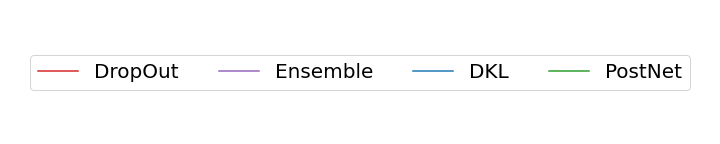
\includegraphics[width=\textwidth]{sections/011_icml2022/resources/legend.png}
    \end{subfigure}
    \vspace{-5mm}
    
    \begin{subfigure}{.24\textwidth}
        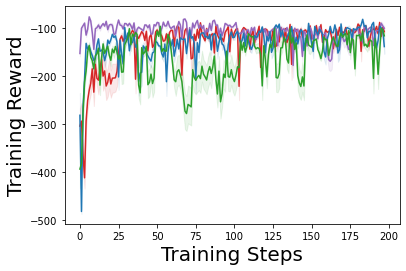
\includegraphics[width=\textwidth]{sections/011_icml2022/resources/acrobot-training_total_reward-training-model.png}
    \end{subfigure}
    \begin{subfigure}{.24\textwidth}
        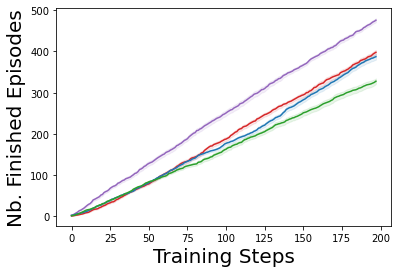
\includegraphics[width=\textwidth]{sections/011_icml2022/resources/acrobot-n_finished_training_episodes-training-model.png}  
    \end{subfigure}
    \begin{subfigure}{.24\textwidth}
        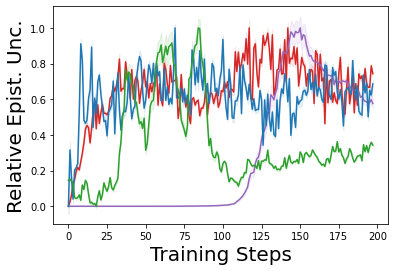
\includegraphics[width=\textwidth]{sections/011_icml2022/resources/acrobot-training_epistemic_uncertainty-training-model.png}
    \end{subfigure}
    \begin{subfigure}{.24\textwidth}
        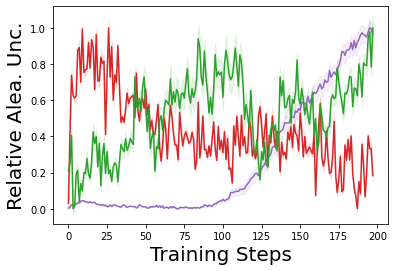
\includegraphics[width=\textwidth]{sections/011_icml2022/resources/acrobot-training_aleatoric_ucertainty-training-model.png}  
    \end{subfigure}
    \vspace{-3mm}
    \caption*{Acrobot}
    \vspace{2mm}

    \begin{subfigure}{.24\textwidth}
        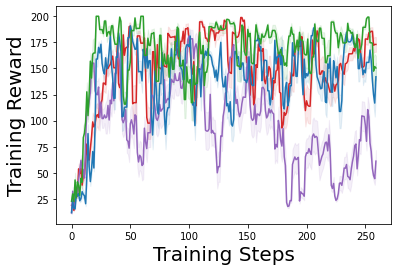
\includegraphics[width=\textwidth]{sections/011_icml2022/resources/cartpole-training_total_reward-training-model.png}
    \end{subfigure}
    \begin{subfigure}{.24\textwidth}
        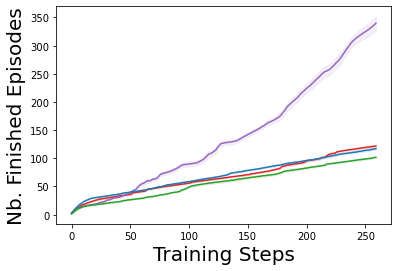
\includegraphics[width=\textwidth]{sections/011_icml2022/resources/cartpole-n_finished_training_episodes-training-model.png}  
    \end{subfigure}
    \begin{subfigure}{.24\textwidth}
        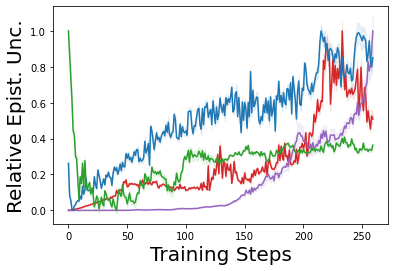
\includegraphics[width=\textwidth]{sections/011_icml2022/resources/cartpole-training_epistemic_uncertainty-training-model.png}
    \end{subfigure}
    \begin{subfigure}{.24\textwidth}
        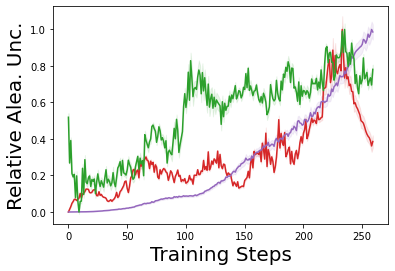
\includegraphics[width=\textwidth]{sections/011_icml2022/resources/cartpole-training_aleatoric_ucertainty-training-model.png}  
    \end{subfigure}
    \vspace{-3mm}
    \caption*{CartPole}
    \vspace{2mm}
    
    \begin{subfigure}{.24\textwidth}
        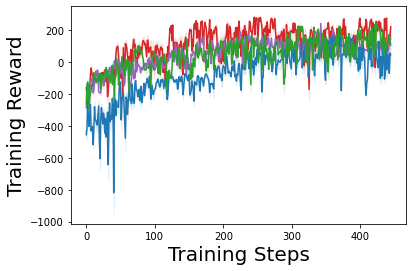
\includegraphics[width=\textwidth]{sections/011_icml2022/resources/lunarlander-training_total_reward-training-model.png}
    \end{subfigure}
    \begin{subfigure}{.24\textwidth}
        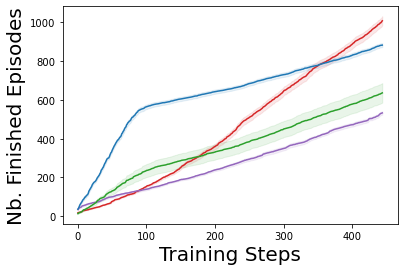
\includegraphics[width=\textwidth]{sections/011_icml2022/resources/lunarlander-n_finished_training_episodes-training-model.png}  
    \end{subfigure}
    \begin{subfigure}{.24\textwidth}
        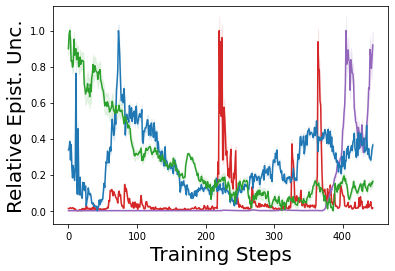
\includegraphics[width=\textwidth]{sections/011_icml2022/resources/lunarlander-training_epistemic_uncertainty-training-model.png}
    \end{subfigure}
    \begin{subfigure}{.24\textwidth}
        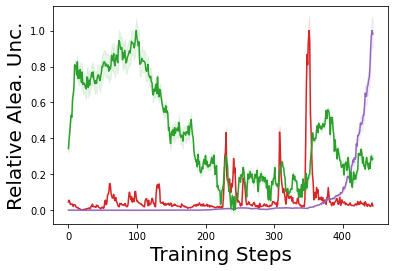
\includegraphics[width=\textwidth]{sections/011_icml2022/resources/lunarlander-training_aleatoric_ucertainty-training-model.png}  
    \end{subfigure}
    \vspace{-3mm}
    \caption*{LunarLander}
    \vspace{2mm}

    \caption{Comparison of the training performance of the four uncertainty methods using epsilon-greedy strategies. Ideally, an uncertainty aware model should achieve high reward with few samples and with a decreasing epistemic uncertainty.}
    \label{fig:model-training-performance}
\end{figure}
%\begin{figure}
    \centering
        \begin{subfigure}{.5\textwidth}
        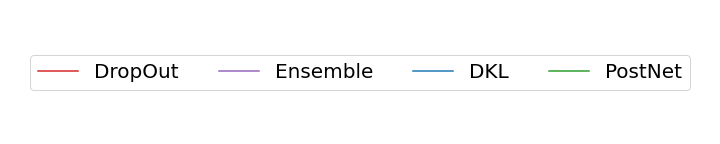
\includegraphics[width=\textwidth]{sections/011_icml2022/resources/legend.png}
    \end{subfigure}
    \vspace{-5mm}
    
    \begin{subfigure}{.245\textwidth}
        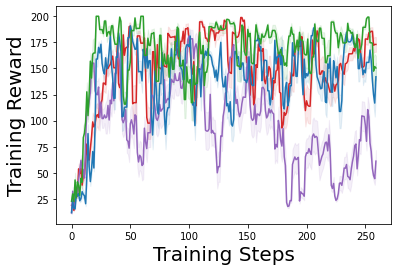
\includegraphics[width=\textwidth]{sections/011_icml2022/resources/cartpole-training_total_reward-training-model.png}
    \end{subfigure}
    \begin{subfigure}{.245\textwidth}
        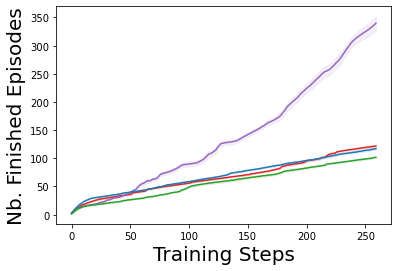
\includegraphics[width=\textwidth]{sections/011_icml2022/resources/cartpole-n_finished_training_episodes-training-model.png}  
    \end{subfigure}
    \begin{subfigure}{.245\textwidth}
        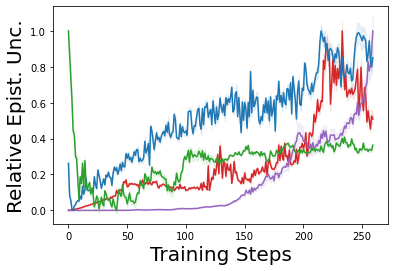
\includegraphics[width=\textwidth]{sections/011_icml2022/resources/cartpole-training_epistemic_uncertainty-training-model.png}
    \end{subfigure}
    \begin{subfigure}{.245\textwidth}
        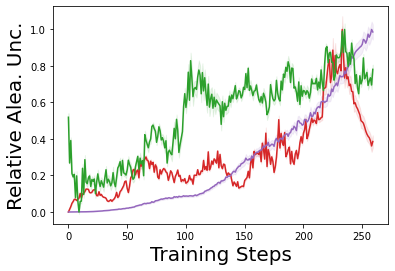
\includegraphics[width=\textwidth]{sections/011_icml2022/resources/cartpole-training_aleatoric_ucertainty-training-model.png}  
    \end{subfigure}
    \caption{Comparison of the training performance of the four uncertainty methods using epsilon-greedy strategies on CartPole. Ideally, a uncertainty aware-model should achieve high reward with few samples and episodes and with a decreasing epistemic uncertainty.}
    \label{fig:model-training-performance-cartpole}
\end{figure}
%\begin{figure}
    \centering
        \begin{subfigure}{.5\textwidth}
        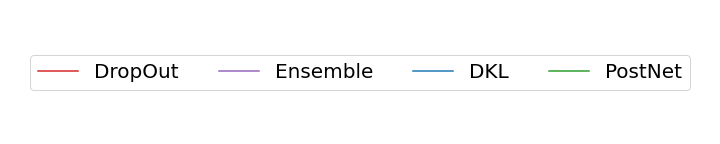
\includegraphics[width=\textwidth]{sections/011_icml2022/resources/legend.png}
    \end{subfigure}
    \vspace{-5mm}
    
    \begin{subfigure}{.245\textwidth}
        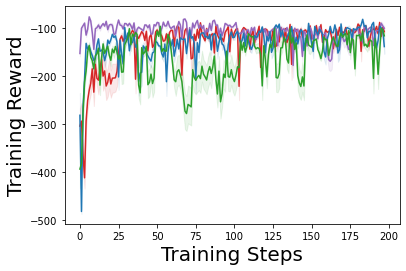
\includegraphics[width=\textwidth]{sections/011_icml2022/resources/acrobot-training_total_reward-training-model.png}
    \end{subfigure}
    \begin{subfigure}{.245\textwidth}
        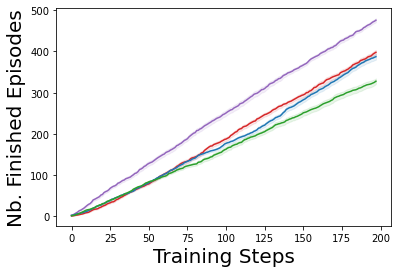
\includegraphics[width=\textwidth]{sections/011_icml2022/resources/acrobot-n_finished_training_episodes-training-model.png}  
    \end{subfigure}
    \begin{subfigure}{.245\textwidth}
        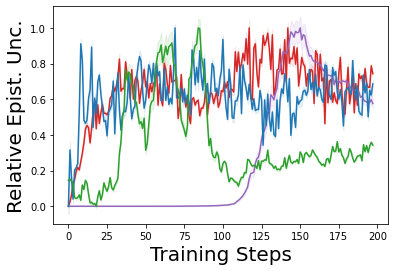
\includegraphics[width=\textwidth]{sections/011_icml2022/resources/acrobot-training_epistemic_uncertainty-training-model.png}
    \end{subfigure}
    \begin{subfigure}{.245\textwidth}
        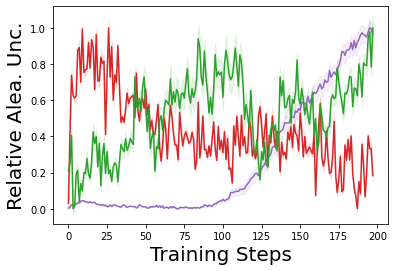
\includegraphics[width=\textwidth]{sections/011_icml2022/resources/acrobot-training_aleatoric_ucertainty-training-model.png}  
    \end{subfigure}
    \caption{Comparison of the training performance of the four uncertainty methods using epsilon-greedy strategies on Acrobot. Ideally, a uncertainty aware-model should achieve high reward with few samples and with a decreasing epistemic uncertainty.}
    \label{fig:model-training-performance-acrobot}
\end{figure}
%\begin{figure}
    \centering
        \begin{subfigure}{.5\textwidth}
        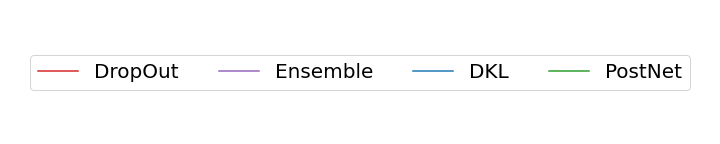
\includegraphics[width=\textwidth]{sections/011_icml2022/resources/legend.png}
    \end{subfigure}
    \vspace{-5mm}
    
    \begin{subfigure}{.245\textwidth}
        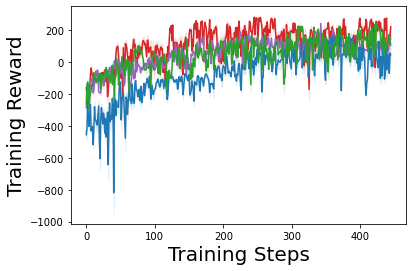
\includegraphics[width=\textwidth]{sections/011_icml2022/resources/lunarlander-training_total_reward-training-model.png}
    \end{subfigure}
    \begin{subfigure}{.245\textwidth}
        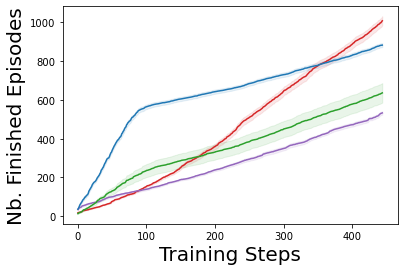
\includegraphics[width=\textwidth]{sections/011_icml2022/resources/lunarlander-n_finished_training_episodes-training-model.png}  
    \end{subfigure}
    \begin{subfigure}{.245\textwidth}
        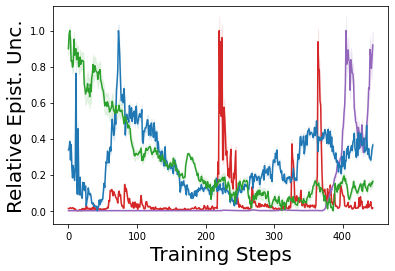
\includegraphics[width=\textwidth]{sections/011_icml2022/resources/lunarlander-training_epistemic_uncertainty-training-model.png}
    \end{subfigure}
    \begin{subfigure}{.245\textwidth}
        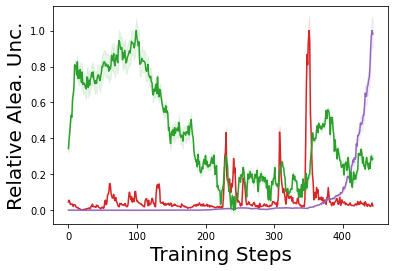
\includegraphics[width=\textwidth]{sections/011_icml2022/resources/lunarlander-training_aleatoric_ucertainty-training-model.png}  
    \end{subfigure}
    \caption{Comparison of the training performance of the four uncertainty methods using epsilon-greedy strategies on LunarLander. Ideally, a uncertainty aware-model should achieve high reward  with few samples and episodes and with a decreasing epistemic uncertainty.}
    \label{fig:model-training-performance-lunarlander}
\end{figure}

We show additional results in \cref{fig:strategy-training-performance} to compare the performance of the sampling-epistemic and the sampling-aleatoric strategies at training time. The sampling-epistemic strategy consistently achieve a better sample efficiency. Thus, Ensemble, DropOut and PostNet empirically satisfy des.~\ref{ax:training_strategy}. Hence, disentangling aleatoric and epistemic uncertainty can speed learning in a training environment.

\begin{figure}
    \centering
    \begin{subfigure}{.45\textwidth}
        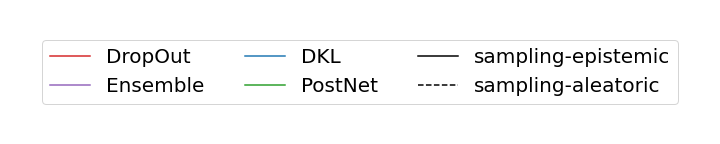
\includegraphics[width=\textwidth]{sections/011_icml2022/resources/sampling-legend.png}
    \end{subfigure}
    \vspace{-3mm}
    
    \begin{subfigure}{.24\textwidth}
        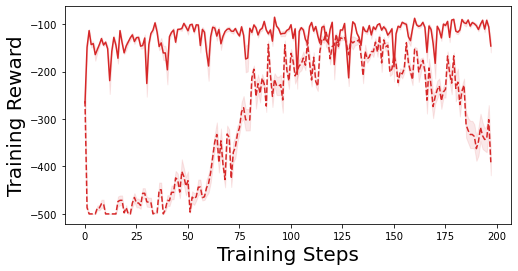
\includegraphics[width=\textwidth]{sections/011_icml2022/resources/acrobot-training_total_reward-dropout-training-strategy.png}
    \end{subfigure}
    \begin{subfigure}{.24\textwidth}
        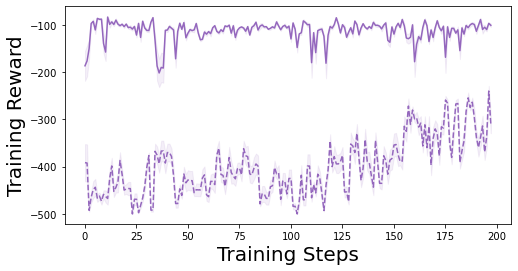
\includegraphics[width=\textwidth]{sections/011_icml2022/resources/acrobot-training_total_reward-ensemble-training-strategy.png}
    \end{subfigure}
    \begin{subfigure}{.24\textwidth}
        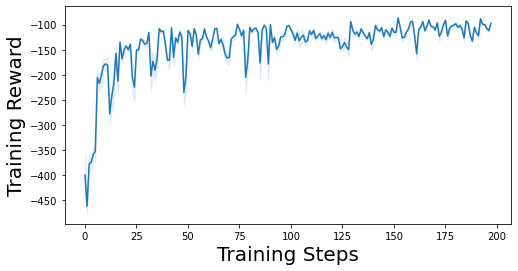
\includegraphics[width=\textwidth]{sections/011_icml2022/resources/acrobot-training_total_reward-dkl-training-strategy.png}
    \end{subfigure}
    \begin{subfigure}{.24\textwidth}
        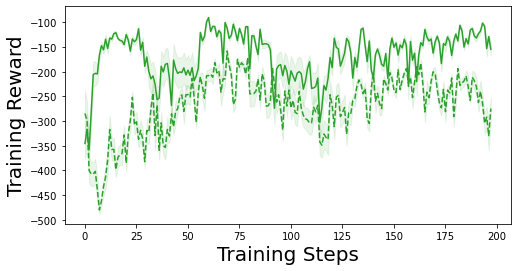
\includegraphics[width=\textwidth]{sections/011_icml2022/resources/acrobot-training_total_reward-postnet-training-strategy.png}
    \end{subfigure}
    
    \begin{subfigure}{.24\textwidth}
        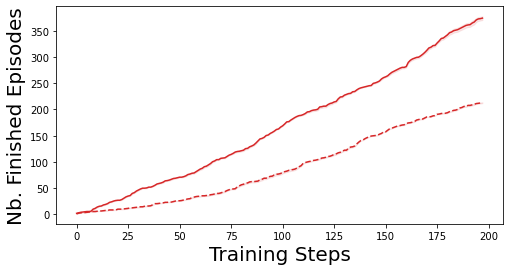
\includegraphics[width=\textwidth]{sections/011_icml2022/resources/acrobot-n_finished_training_episodes-dropout-training-strategy.png}
    \end{subfigure}
    \begin{subfigure}{.24\textwidth}
        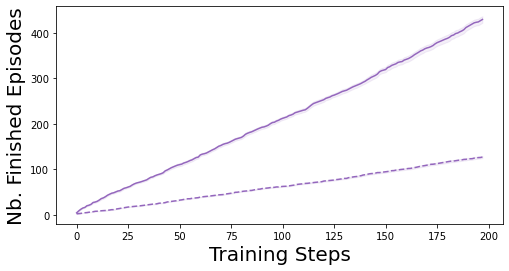
\includegraphics[width=\textwidth]{sections/011_icml2022/resources/acrobot-n_finished_training_episodes-ensemble-training-strategy.png}
    \end{subfigure}
    \begin{subfigure}{.24\textwidth}
        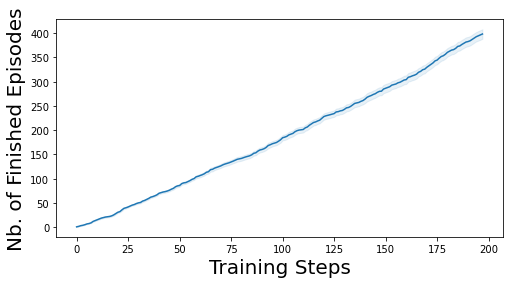
\includegraphics[width=\textwidth]{sections/011_icml2022/resources/acrobot-n_finished_training_episodes-dkl-training-strategy.png}
    \end{subfigure}
    \begin{subfigure}{.24\textwidth}
        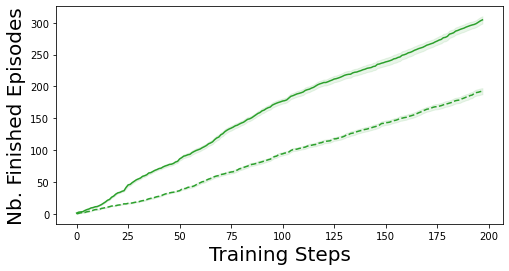
\includegraphics[width=\textwidth]{sections/011_icml2022/resources/acrobot-n_finished_training_episodes-postnet-training-strategy.png}
    \end{subfigure}
    \vspace{-3mm}
    \caption*{CartPole}
    \vspace{2mm}
    
    \begin{subfigure}{.24\textwidth}
        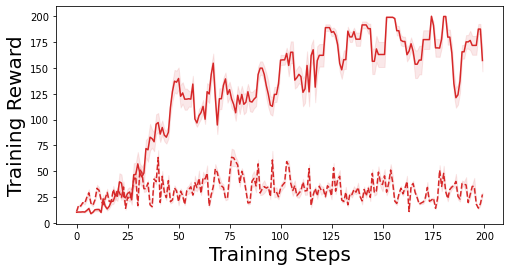
\includegraphics[width=\textwidth]{sections/011_icml2022/resources/cartpole-training_total_reward-dropout-training-strategy.png}
    \end{subfigure}
    \begin{subfigure}{.24\textwidth}
        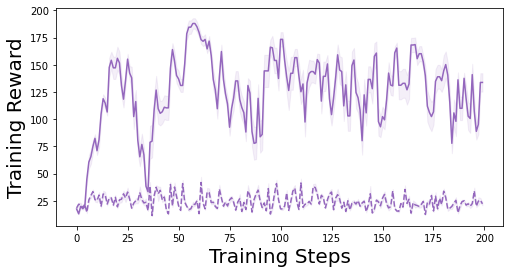
\includegraphics[width=\textwidth]{sections/011_icml2022/resources/cartpole-training_total_reward-ensemble-training-strategy.png}
    \end{subfigure}
    \begin{subfigure}{.24\textwidth}
        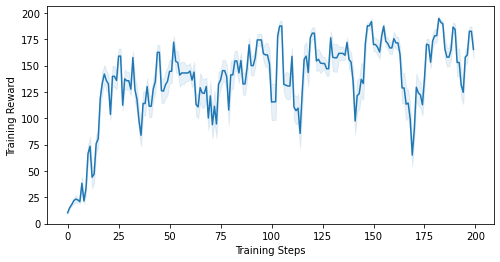
\includegraphics[width=\textwidth]{sections/011_icml2022/resources/cartpole-training_total_reward-dkl-training-strategy.png}
    \end{subfigure}
    \begin{subfigure}{.24\textwidth}
        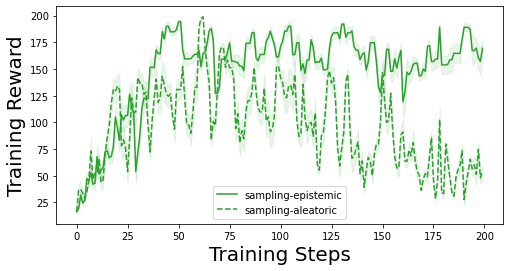
\includegraphics[width=\textwidth]{sections/011_icml2022/resources/cartpole-training_total_reward-postnet-training-strategy.png}
    \end{subfigure}
    
    \begin{subfigure}{.24\textwidth}
        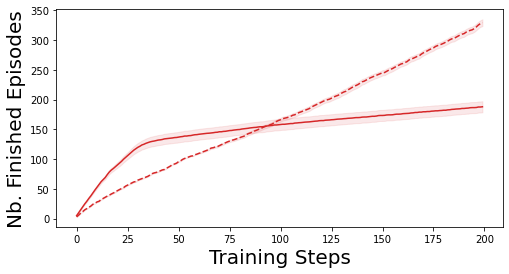
\includegraphics[width=\textwidth]{sections/011_icml2022/resources/cartpole-n_finished_training_episodes-dropout-training-strategy.png}
    \end{subfigure}
    \begin{subfigure}{.24\textwidth}
        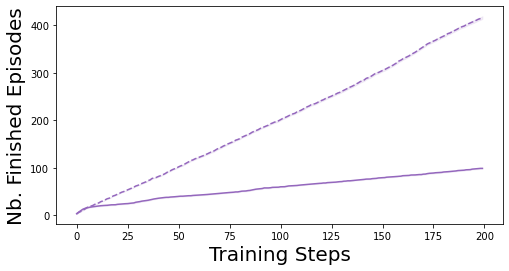
\includegraphics[width=\textwidth]{sections/011_icml2022/resources/cartpole-n_finished_training_episodes-ensemble-training-strategy.png}
    \end{subfigure}
    \begin{subfigure}{.24\textwidth}
        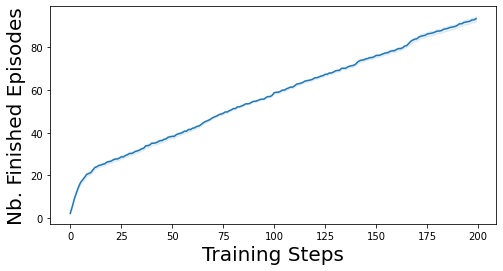
\includegraphics[width=\textwidth]{sections/011_icml2022/resources/cartpole-n_finished_training_episodes-dkl-training-strategy.png}
    \end{subfigure}
    \begin{subfigure}{.24\textwidth}
        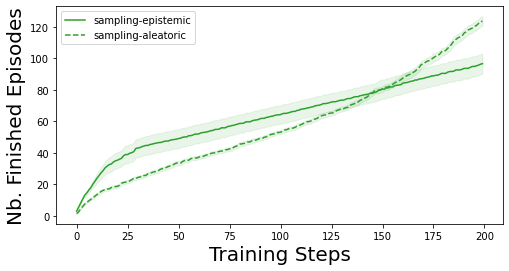
\includegraphics[width=\textwidth]{sections/011_icml2022/resources/cartpole-n_finished_training_episodes-postnet-training-strategy.png}
    \end{subfigure}
    \vspace{-3mm}
    \caption*{Acrobot}
    \vspace{2mm}

    \begin{subfigure}{.24\textwidth}
        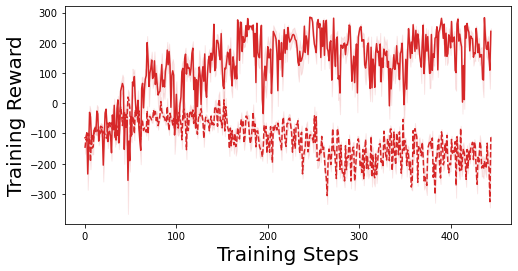
\includegraphics[width=\textwidth]{sections/011_icml2022/resources/lunarlander-training_total_reward-dropout-training-strategy.png}
    \end{subfigure}
    \begin{subfigure}{.24\textwidth}
        \includegraphics[width=\textwidth]{sections/011_icml2022/resources/lunarlander-training_total_reward-ensemble-training-strategy.png}
    \end{subfigure}
    \begin{subfigure}{.24\textwidth}
        \includegraphics[width=\textwidth]{sections/011_icml2022/resources/lunarlander-training_total_reward-dkl-training-strategy.png}
    \end{subfigure}
    \begin{subfigure}{.24\textwidth}
        \includegraphics[width=\textwidth]{sections/011_icml2022/resources/lunarlander-training_total_reward-postnet-training-strategy.png}
    \end{subfigure}
    
    \begin{subfigure}{.24\textwidth}
        \includegraphics[width=\textwidth]{sections/011_icml2022/resources/lunarlander-n_finished_training_episodes-dropout-training-strategy.png}
    \end{subfigure}
    \begin{subfigure}{.24\textwidth}
        \includegraphics[width=\textwidth]{sections/011_icml2022/resources/lunarlander-n_finished_training_episodes-ensemble-training-strategy.png}
    \end{subfigure}
    \begin{subfigure}{.24\textwidth}
        \includegraphics[width=\textwidth]{sections/011_icml2022/resources/lunarlander-n_finished_training_episodes-dkl-training-strategy.png}
    \end{subfigure}
    \begin{subfigure}{.24\textwidth}
        \includegraphics[width=\textwidth]{sections/011_icml2022/resources/lunarlander-n_finished_training_episodes-postnet-training-strategy.png}
    \end{subfigure}
    \vspace{-3mm}
    \caption*{LunarLander}
    \vspace{2mm}
    
    \caption{Comparison of the training performance. The four uncertainty methods use the sampling-aleatoric or the sampling-epistemic at training time. Ideally, an uncertainty aware-model should high reward with few samples.}
    \label{fig:strategy-training-performance}
\end{figure}
%\begin{figure}
    \centering
    \begin{subfigure}{.45\textwidth}
        \includegraphics[width=\textwidth]{sections/011_icml2022/resources/sampling-legend.png}
    \end{subfigure}
    \vspace{-3mm}
    
    \begin{subfigure}{.245\textwidth}
        \includegraphics[width=\textwidth]{sections/011_icml2022/resources/cartpole-training_total_reward-dropout-training-strategy.png}
    \end{subfigure}
    \begin{subfigure}{.245\textwidth}
        \includegraphics[width=\textwidth]{sections/011_icml2022/resources/cartpole-training_total_reward-ensemble-training-strategy.png}
    \end{subfigure}
    \begin{subfigure}{.245\textwidth}
        \includegraphics[width=\textwidth]{sections/011_icml2022/resources/cartpole-training_total_reward-dkl-training-strategy.png}
    \end{subfigure}
    \begin{subfigure}{.245\textwidth}
        \includegraphics[width=\textwidth]{sections/011_icml2022/resources/cartpole-training_total_reward-postnet-training-strategy.png}
    \end{subfigure}
    
    \begin{subfigure}{.245\textwidth}
        \includegraphics[width=\textwidth]{sections/011_icml2022/resources/cartpole-n_finished_training_episodes-dropout-training-strategy.png}
    \end{subfigure}
    \begin{subfigure}{.245\textwidth}
        \includegraphics[width=\textwidth]{sections/011_icml2022/resources/cartpole-n_finished_training_episodes-ensemble-training-strategy.png}
    \end{subfigure}
    \begin{subfigure}{.245\textwidth}
        \includegraphics[width=\textwidth]{sections/011_icml2022/resources/cartpole-n_finished_training_episodes-dkl-training-strategy.png}
    \end{subfigure}
    \begin{subfigure}{.245\textwidth}
        \includegraphics[width=\textwidth]{sections/011_icml2022/resources/cartpole-n_finished_training_episodes-postnet-training-strategy.png}
    \end{subfigure}
    \caption{Comparison of the training performance on Cartpole. The four uncertainty methods use the sampling-aleatoric or the sampling-epistemic at training time. Ideally, an uncertainty aware-model should high reward with few samples.}
    \label{fig:strategy-training-performance-cartpole}
\end{figure}
%\begin{figure}
    \centering
    \begin{subfigure}{.45\textwidth}
        \includegraphics[width=\textwidth]{sections/011_icml2022/resources/sampling-legend.png}
    \end{subfigure}
    \vspace{-3mm}
    
    \begin{subfigure}{.245\textwidth}
        \includegraphics[width=\textwidth]{sections/011_icml2022/resources/acrobot-training_total_reward-dropout-training-strategy.png}
    \end{subfigure}
    \begin{subfigure}{.245\textwidth}
        \includegraphics[width=\textwidth]{sections/011_icml2022/resources/acrobot-training_total_reward-ensemble-training-strategy.png}
    \end{subfigure}
    \begin{subfigure}{.245\textwidth}
        \includegraphics[width=\textwidth]{sections/011_icml2022/resources/acrobot-training_total_reward-dkl-training-strategy.png}
    \end{subfigure}
    \begin{subfigure}{.245\textwidth}
        \includegraphics[width=\textwidth]{sections/011_icml2022/resources/acrobot-training_total_reward-postnet-training-strategy.png}
    \end{subfigure}
    
    \begin{subfigure}{.245\textwidth}
        \includegraphics[width=\textwidth]{sections/011_icml2022/resources/acrobot-n_finished_training_episodes-dropout-training-strategy.png}
    \end{subfigure}
    \begin{subfigure}{.245\textwidth}
        \includegraphics[width=\textwidth]{sections/011_icml2022/resources/acrobot-n_finished_training_episodes-ensemble-training-strategy.png}
    \end{subfigure}
    \begin{subfigure}{.245\textwidth}
        \includegraphics[width=\textwidth]{sections/011_icml2022/resources/acrobot-n_finished_training_episodes-dkl-training-strategy.png}
    \end{subfigure}
    \begin{subfigure}{.245\textwidth}
        \includegraphics[width=\textwidth]{sections/011_icml2022/resources/acrobot-n_finished_training_episodes-postnet-training-strategy.png}
    \end{subfigure}
    \caption{Comparison of the training performance on Acrobot. The four uncertainty methods use the sampling-aleatoric or the sampling-epistemic at training time. Ideally, an uncertainty aware-model should high reward with few samples.}
    \label{fig:strategy-training-performance-acrobot}
\end{figure}
%\begin{figure}
    \centering
    \begin{subfigure}{.45\textwidth}
        \includegraphics[width=\textwidth]{sections/011_icml2022/resources/sampling-legend.png}
    \end{subfigure}
    \vspace{-3mm}
    
    \begin{subfigure}{.245\textwidth}
        \includegraphics[width=\textwidth]{sections/011_icml2022/resources/lunarlander-training_total_reward-dropout-training-strategy.png}
    \end{subfigure}
    \begin{subfigure}{.245\textwidth}
        \includegraphics[width=\textwidth]{sections/011_icml2022/resources/lunarlander-training_total_reward-ensemble-training-strategy.png}
    \end{subfigure}
    \begin{subfigure}{.245\textwidth}
        \includegraphics[width=\textwidth]{sections/011_icml2022/resources/lunarlander-training_total_reward-dkl-training-strategy.png}
    \end{subfigure}
    \begin{subfigure}{.245\textwidth}
        \includegraphics[width=\textwidth]{sections/011_icml2022/resources/lunarlander-training_total_reward-postnet-training-strategy.png}
    \end{subfigure}
    
    \begin{subfigure}{.245\textwidth}
        \includegraphics[width=\textwidth]{sections/011_icml2022/resources/lunarlander-n_finished_training_episodes-dropout-training-strategy.png}
    \end{subfigure}
    \begin{subfigure}{.245\textwidth}
        \includegraphics[width=\textwidth]{sections/011_icml2022/resources/lunarlander-n_finished_training_episodes-ensemble-training-strategy.png}
    \end{subfigure}
    \begin{subfigure}{.245\textwidth}
        \includegraphics[width=\textwidth]{sections/011_icml2022/resources/lunarlander-n_finished_training_episodes-dkl-training-strategy.png}
    \end{subfigure}
    \begin{subfigure}{.245\textwidth}
        \includegraphics[width=\textwidth]{sections/011_icml2022/resources/lunarlander-n_finished_training_episodes-postnet-training-strategy.png}
    \end{subfigure}
    \caption{Comparison of the training performance on LunarLander. The four uncertainty methods use the sampling-aleatoric or the sampling-epistemic at training time. Ideally, an uncertainty aware-model should high reward with few samples.}
    \label{fig:strategy-training-performance-lunarlander}
\end{figure}

\subsection{Testing Time}

We show additional results in \cref{fig:model-testing-performance} to compare the generalization and OOD detection performance of the uncertainty estimates of the four uncertainty methods at testing time. The models use the sampling-epistemic or the sampling-aleatoric strategy at both training and testing time. Further, we show other additional results for OOD detection by using the area under the precision-recall (AUC-PR) scores instead of the area under the receiver operating characteristic curve (AUC-ROC) in \cref{fig:strategy-testing-ood-auc-pr-performance}. We observe that DKL and PostNet achieve  very high OOD detection scores in most settings  compared to DropOut and Ensemble. These \emph{empirical} results align with the \emph{theoretical} results stating that DKL and PostNet should assign high uncertainty to states very different from states observed during training. Thus, DKL and PostNet validate des.~\ref{ax:testing_state}. In particular, DKL and PostNet can reliably equip DQN with epistemic uncertainty estimates which can be used to flag anomalous OOD states.

\begin{figure}
    \centering
        \begin{subfigure}{.5\textwidth}
        \includegraphics[width=\textwidth]{sections/011_icml2022/resources/legend.png}
    \end{subfigure}
    \vspace{-5mm}
    
    \begin{subfigure}{.4\textwidth}
        \includegraphics[width=\textwidth]{sections/011_icml2022/resources/Acrobot-v1-mean_reward_-testing-model.png}  
    \end{subfigure}
    \begin{subfigure}{.4\textwidth}
        \includegraphics[width=\textwidth]{sections/011_icml2022/resources/AcrobotOOD-v0-AUC-ROC-epistemic_-testing-model.png}
    \end{subfigure}
        \vspace{-3mm}
    \caption*{Acrobot}
    \vspace{2mm}

    \begin{subfigure}{.4\textwidth}
        \includegraphics[width=\textwidth]{sections/011_icml2022/resources/CartPole-v0-mean_reward_-testing-model.png}  
    \end{subfigure}
    \begin{subfigure}{.4\textwidth}
        \includegraphics[width=\textwidth]{sections/011_icml2022/resources/CartPoleOOD-v0-AUC-ROC-epistemic_-testing-model.png}
    \end{subfigure}
        \vspace{-3mm}
    \caption*{CartPole}
    \vspace{2mm}

    \begin{subfigure}{.4\textwidth}
        \includegraphics[width=\textwidth]{sections/011_icml2022/resources/LunarLander-v2-mean_reward_-testing-model.png}  
    \end{subfigure}
    \begin{subfigure}{.4\textwidth}
        \includegraphics[width=\textwidth]{sections/011_icml2022/resources/LunarLanderOOD-v0-AUC-ROC-epistemic_-testing-model.png}
    \end{subfigure}
        \vspace{-3mm}
    \caption*{LunarLander}
    \vspace{2mm}
    
    \caption{Comparison of the testing performance of the four uncertainty methods using epsilon-greedy strategies at training and testing time. Ideally, an uncertainty aware model should achieve high reward and high OOD detection scores.}
    \label{fig:model-testing-performance}
\end{figure}
%\begin{figure}
    \centering
    \vspace{-7mm}
        \begin{subfigure}{.5\textwidth}
        \includegraphics[width=\textwidth]{sections/011_icml2022/resources/legend.png}
    \end{subfigure}
    \vspace{-5mm}
    
    \begin{subfigure}{.4\textwidth}
        \includegraphics[width=\textwidth]{sections/011_icml2022/resources/CartPole-v0-mean_reward_-testing-model.png}  
    \end{subfigure}
    \begin{subfigure}{.4\textwidth}
        \includegraphics[width=\textwidth]{sections/011_icml2022/resources/CartPoleOOD-v0-AUC-ROC-epistemic_-testing-model.png}
    \end{subfigure}
        \vspace{-3mm}
    \caption{Comparison of the testing performance of the four uncertainty methods using epsilon-greedy strategies at training and testing time on CartPole. Ideally, an uncertainty aware-model should achieve high reward and high OOD detection scores.}
    \label{fig:model-testing-performance-cartpole}
    \vspace{-4mm}
\end{figure}
%\begin{figure}
    \centering
        \begin{subfigure}{.5\textwidth}
        \includegraphics[width=\textwidth]{sections/011_icml2022/resources/legend.png}
    \end{subfigure}
    \vspace{-5mm}
    
    \begin{subfigure}{.4\textwidth}
        \includegraphics[width=\textwidth]{sections/011_icml2022/resources/Acrobot-v1-mean_reward_-testing-model.png}  
    \end{subfigure}
    \begin{subfigure}{.4\textwidth}
        \includegraphics[width=\textwidth]{sections/011_icml2022/resources/AcrobotOOD-v0-AUC-ROC-epistemic_-testing-model.png}
    \end{subfigure}
    \caption{Comparison of the testing performance of the four uncertainty methods using epsilon-greedy strategies at training and testing time on Acrobot. Ideally, an uncertainty aware-model should achieve high reward and high OOD detection scores.}
    \label{fig:model-testing-performance-acrobot}
\end{figure}
%\begin{figure}
    \centering
        \begin{subfigure}{.5\textwidth}
        \includegraphics[width=\textwidth]{sections/011_icml2022/resources/legend.png}
    \end{subfigure}
    \vspace{-5mm}
    
    \begin{subfigure}{.4\textwidth}
        \includegraphics[width=\textwidth]{sections/011_icml2022/resources/LunarLander-v2-mean_reward_-testing-model.png}  
    \end{subfigure}
    \begin{subfigure}{.4\textwidth}
        \includegraphics[width=\textwidth]{sections/011_icml2022/resources/LunarLanderOOD-v0-AUC-ROC-epistemic_-testing-model.png}
    \end{subfigure}
    \caption{Comparison of the testing performance of the four uncertainty methods using epsilon-greedy strategies at training and testing time on LunarLander. Ideally, an uncertainty aware-model should achieve high reward and high OOD detection scores.}
    \label{fig:model-testing-performance-lunarlander}
\end{figure}

We show additional results in \cref{fig:strategy-testing-performance} to compare the performance of the sampling-epistemic and sampling-aleatoric strategies for each uncertainty model. All models use the same epsilon-greedy strategy at training time. We observe that the sampling-epistemic strategy is consistently better than sampling-aleatoric at testing time. The higher generalization capacity of the sampling-epistemic strategy aligns with \citep{epistemic-pomdp} which recasts the problem of generalization in RL as solving an epistemic POMDP. These empirical results underline the need to disentangle both aleatoric and epistemic uncertainty for high reward performance at testing time.

\begin{figure}
    \centering
    \begin{subfigure}{.45\textwidth}
        \includegraphics[width=\textwidth]{sections/011_icml2022/resources/sampling-legend.png}
    \end{subfigure}
    \vspace{-3mm}
    
    \begin{subfigure}{.24\textwidth}
        \includegraphics[width=\textwidth]{sections/011_icml2022/resources/DropOut-Acrobot-v1-mean_reward_-testing-strategy.png}
    \end{subfigure}
    \begin{subfigure}{.24\textwidth}
        \includegraphics[width=\textwidth]{sections/011_icml2022/resources/Ensemble-Acrobot-v1-mean_reward_-testing-strategy.png}
    \end{subfigure}
    \begin{subfigure}{.24\textwidth}
        \includegraphics[width=\textwidth]{sections/011_icml2022/resources/DKL-Acrobot-v1-mean_reward_-testing-strategy.png}
    \end{subfigure}
    \begin{subfigure}{.24\textwidth}
        \includegraphics[width=\textwidth]{sections/011_icml2022/resources/PostNet-Acrobot-v1-mean_reward_-testing-strategy.png}
    \end{subfigure}
    
    \begin{subfigure}{.24\textwidth}
        \includegraphics[width=\textwidth]{sections/011_icml2022/resources/DropOut-AcrobotOOD-v0-AUC-ROC-epistemic_-testing-strategy.png}
    \end{subfigure}
    \begin{subfigure}{.24\textwidth}
        \includegraphics[width=\textwidth]{sections/011_icml2022/resources/Ensemble-AcrobotOOD-v0-AUC-ROC-epistemic_-testing-strategy.png}
    \end{subfigure}
    \begin{subfigure}{.24\textwidth}
        \includegraphics[width=\textwidth]{sections/011_icml2022/resources/DKL-AcrobotOOD-v0-AUC-ROC-epistemic_-testing-strategy.png}
    \end{subfigure}
    \begin{subfigure}{.24\textwidth}
        \includegraphics[width=\textwidth]{sections/011_icml2022/resources/PostNet-AcrobotOOD-v0-AUC-ROC-epistemic_-testing-strategy.png}
    \end{subfigure}
    \vspace{-3mm}
    \caption*{Acrobot}
    \vspace{2mm}

    \begin{subfigure}{.24\textwidth}
        \includegraphics[width=\textwidth]{sections/011_icml2022/resources/DropOut-CartPole-v0-mean_reward_-testing-strategy.png}
    \end{subfigure}
    \begin{subfigure}{.24\textwidth}
        \includegraphics[width=\textwidth]{sections/011_icml2022/resources/Ensemble-CartPole-v0-mean_reward_-testing-strategy.png}
    \end{subfigure}
    \begin{subfigure}{.24\textwidth}
        \includegraphics[width=\textwidth]{sections/011_icml2022/resources/DKL-CartPole-v0-mean_reward_-testing-strategy.png}
    \end{subfigure}
    \begin{subfigure}{.24\textwidth}
        \includegraphics[width=\textwidth]{sections/011_icml2022/resources/PostNet-CartPole-v0-mean_reward_-testing-strategy.png}
    \end{subfigure}
    
    \begin{subfigure}{.24\textwidth}
        \includegraphics[width=\textwidth]{sections/011_icml2022/resources/DropOut-CartPoleOOD-v0-AUC-ROC-epistemic_-testing-strategy.png}
    \end{subfigure}
    \begin{subfigure}{.24\textwidth}
        \includegraphics[width=\textwidth]{sections/011_icml2022/resources/Ensemble-CartPoleOOD-v0-AUC-ROC-epistemic_-testing-strategy.png}
    \end{subfigure}
    \begin{subfigure}{.24\textwidth}
        \includegraphics[width=\textwidth]{sections/011_icml2022/resources/DKL-CartPoleOOD-v0-AUC-ROC-epistemic_-testing-strategy.png}
    \end{subfigure}
    \begin{subfigure}{.24\textwidth}
        \includegraphics[width=\textwidth]{sections/011_icml2022/resources/PostNet-CartPoleOOD-v0-AUC-ROC-epistemic_-testing-strategy.png}
    \end{subfigure}
    \vspace{-3mm}
    \caption*{CartPole}
    \vspace{2mm}

    \begin{subfigure}{.24\textwidth}
        \includegraphics[width=\textwidth]{sections/011_icml2022/resources/DropOut-LunarLander-v2-mean_reward_-testing-strategy.png}
    \end{subfigure}
    \begin{subfigure}{.24\textwidth}
        \includegraphics[width=\textwidth]{sections/011_icml2022/resources/Ensemble-LunarLander-v2-mean_reward_-testing-strategy.png}
    \end{subfigure}
    \begin{subfigure}{.24\textwidth}
        \includegraphics[width=\textwidth]{sections/011_icml2022/resources/DKL-LunarLander-v2-mean_reward_-testing-strategy.png}
    \end{subfigure}
    \begin{subfigure}{.24\textwidth}
        \includegraphics[width=\textwidth]{sections/011_icml2022/resources/PostNet-LunarLander-v2-mean_reward_-testing-strategy.png}
    \end{subfigure}
    
    \begin{subfigure}{.24\textwidth}
        \includegraphics[width=\textwidth]{sections/011_icml2022/resources/DropOut-LunarLanderOOD-v0-AUC-ROC-epistemic_-testing-strategy.png}
    \end{subfigure}
    \begin{subfigure}{.24\textwidth}
        \includegraphics[width=\textwidth]{sections/011_icml2022/resources/Ensemble-LunarLanderOOD-v0-AUC-ROC-epistemic_-testing-strategy.png}
    \end{subfigure}
    \begin{subfigure}{.24\textwidth}
        \includegraphics[width=\textwidth]{sections/011_icml2022/resources/DKL-LunarLanderOOD-v0-AUC-ROC-epistemic_-testing-strategy.png}
    \end{subfigure}
    \begin{subfigure}{.24\textwidth}
        \includegraphics[width=\textwidth]{sections/011_icml2022/resources/PostNet-LunarLanderOOD-v0-AUC-ROC-epistemic_-testing-strategy.png}
    \end{subfigure}
    \vspace{-3mm}
    \caption*{LunarLander}
    \vspace{2mm}
    
    \caption{Comparison of the testing reward and OOD performance. The four uncertainty methods use the sampling-aleatoric or sampling-epistemic strategies at both training and testing time. Ideally, an uncertainty aware model should achieve high testing reward and high OOD AUC-ROC detection score.}
    \label{fig:strategy-testing-performance}
\end{figure}
%\begin{figure}
    \centering
    \begin{subfigure}{.45\textwidth}
        \includegraphics[width=\textwidth]{sections/011_icml2022/resources/sampling-legend.png}
    \end{subfigure}
    \vspace{-3mm}
    
    \begin{subfigure}{.245\textwidth}
        \includegraphics[width=\textwidth]{sections/011_icml2022/resources/DropOut-CartPole-v0-mean_reward_-testing-strategy.png}
    \end{subfigure}
    \begin{subfigure}{.245\textwidth}
        \includegraphics[width=\textwidth]{sections/011_icml2022/resources/Ensemble-CartPole-v0-mean_reward_-testing-strategy.png}
    \end{subfigure}
    \begin{subfigure}{.245\textwidth}
        \includegraphics[width=\textwidth]{sections/011_icml2022/resources/DKL-CartPole-v0-mean_reward_-testing-strategy.png}
    \end{subfigure}
    \begin{subfigure}{.245\textwidth}
        \includegraphics[width=\textwidth]{sections/011_icml2022/resources/PostNet-CartPole-v0-mean_reward_-testing-strategy.png}
    \end{subfigure}
    
    \begin{subfigure}{.245\textwidth}
        \includegraphics[width=\textwidth]{sections/011_icml2022/resources/DropOut-CartPoleOOD-v0-AUC-ROC-epistemic_-testing-strategy.png}
    \end{subfigure}
    \begin{subfigure}{.245\textwidth}
        \includegraphics[width=\textwidth]{sections/011_icml2022/resources/Ensemble-CartPoleOOD-v0-AUC-ROC-epistemic_-testing-strategy.png}
    \end{subfigure}
    \begin{subfigure}{.245\textwidth}
        \includegraphics[width=\textwidth]{sections/011_icml2022/resources/DKL-CartPoleOOD-v0-AUC-ROC-epistemic_-testing-strategy.png}
    \end{subfigure}
    \begin{subfigure}{.245\textwidth}
        \includegraphics[width=\textwidth]{sections/011_icml2022/resources/PostNet-CartPoleOOD-v0-AUC-ROC-epistemic_-testing-strategy.png}
    \end{subfigure}
    \caption{Comparison of the testing reward and OOD performance on CartPole. The four uncertainty methods use the sampling-aleatoric or sampling-epistemic strategies at both training and testing time. Ideally, an uncertainty aware-model should achieve high testing reward and high OOD AUC-ROC detection score.}
    \label{fig:strategy-testing-performance-cartpole}
\end{figure}
%\begin{figure}
    \centering
    \begin{subfigure}{.45\textwidth}
        \includegraphics[width=\textwidth]{sections/011_icml2022/resources/sampling-legend.png}
    \end{subfigure}
    \vspace{-3mm}
    
    \begin{subfigure}{.245\textwidth}
        \includegraphics[width=\textwidth]{sections/011_icml2022/resources/DropOut-Acrobot-v1-mean_reward_-testing-strategy.png}
    \end{subfigure}
    \begin{subfigure}{.245\textwidth}
        \includegraphics[width=\textwidth]{sections/011_icml2022/resources/Ensemble-Acrobot-v1-mean_reward_-testing-strategy.png}
    \end{subfigure}
    \begin{subfigure}{.245\textwidth}
        \includegraphics[width=\textwidth]{sections/011_icml2022/resources/DKL-Acrobot-v1-mean_reward_-testing-strategy.png}
    \end{subfigure}
    \begin{subfigure}{.245\textwidth}
        \includegraphics[width=\textwidth]{sections/011_icml2022/resources/PostNet-Acrobot-v1-mean_reward_-testing-strategy.png}
    \end{subfigure}
    
    \begin{subfigure}{.245\textwidth}
        \includegraphics[width=\textwidth]{sections/011_icml2022/resources/DropOut-AcrobotOOD-v0-AUC-ROC-epistemic_-testing-strategy.png}
    \end{subfigure}
    \begin{subfigure}{.245\textwidth}
        \includegraphics[width=\textwidth]{sections/011_icml2022/resources/Ensemble-AcrobotOOD-v0-AUC-ROC-epistemic_-testing-strategy.png}
    \end{subfigure}
    \begin{subfigure}{.245\textwidth}
        \includegraphics[width=\textwidth]{sections/011_icml2022/resources/DKL-AcrobotOOD-v0-AUC-ROC-epistemic_-testing-strategy.png}
    \end{subfigure}
    \begin{subfigure}{.245\textwidth}
        \includegraphics[width=\textwidth]{sections/011_icml2022/resources/PostNet-AcrobotOOD-v0-AUC-ROC-epistemic_-testing-strategy.png}
    \end{subfigure}
    \caption{Comparison of the testing reward and OOD performance on Acrobot. The four uncertainty methods use the sampling-aleatoric or sampling-epistemic strategies at both training and testing time. Ideally, an uncertainty aware-model should achieve high testing reward and high OOD AUC-ROC detection score.}
    \label{fig:strategy-testing-performance-acrobot}
\end{figure}
%\begin{figure*}
    \centering
        % \vspace{-6mm}
    \begin{subfigure}{.45\textwidth}
        \includegraphics[width=\textwidth]{sections/011_icml2022/resources/sampling-legend.png}
    \end{subfigure}
    \vspace{-5mm}
    
    \begin{subfigure}{.2\textwidth}
        \includegraphics[width=\textwidth]{sections/011_icml2022/resources/DropOut-LunarLander-v2-mean_reward_-testing-strategy.png}
    \end{subfigure}
    \begin{subfigure}{.2\textwidth}
        \includegraphics[width=\textwidth]{sections/011_icml2022/resources/Ensemble-LunarLander-v2-mean_reward_-testing-strategy.png}
    \end{subfigure}
    \begin{subfigure}{.2\textwidth}
        \includegraphics[width=\textwidth]{sections/011_icml2022/resources/DKL-LunarLander-v2-mean_reward_-testing-strategy.png}
    \end{subfigure}
    \begin{subfigure}{.2\textwidth}
        \includegraphics[width=\textwidth]{sections/011_icml2022/resources/PostNet-LunarLander-v2-mean_reward_-testing-strategy.png}
    \end{subfigure}
    
    \begin{subfigure}{.2\textwidth}
        \includegraphics[width=\textwidth]{sections/011_icml2022/resources/DropOut-LunarLanderOOD-v0-AUC-ROC-epistemic_-testing-strategy.png}
    \end{subfigure}
    \begin{subfigure}{.2\textwidth}
        \includegraphics[width=\textwidth]{sections/011_icml2022/resources/Ensemble-LunarLanderOOD-v0-AUC-ROC-epistemic_-testing-strategy.png}
    \end{subfigure}
    \begin{subfigure}{.2\textwidth}
        \includegraphics[width=\textwidth]{sections/011_icml2022/resources/DKL-LunarLanderOOD-v0-AUC-ROC-epistemic_-testing-strategy.png}
    \end{subfigure}
    \begin{subfigure}{.2\textwidth}
        \includegraphics[width=\textwidth]{sections/011_icml2022/resources/PostNet-LunarLanderOOD-v0-AUC-ROC-epistemic_-testing-strategy.png}
    \end{subfigure}
        % \vspace{-3mm}
    \caption{Comparison of the testing reward and OOD performance on LunarLander. The four uncertainty methods use the sampling-aleatoric or sampling-epistemic strategies at both training and testing time. Ideally, an uncertainty aware-model should achieve high testing reward and high OOD AUC-ROC detection score.}
    \label{fig:strategy-testing-performance-lunarlander}
        % \vspace{-6mm}
\end{figure*}

We show additional results in \cref{fig:strategy-shift-testing-performance-cartpole,fig:strategy-shift-testing-performance-acrobot,fig:strategy-shift-testing-performance-lunarlander} to compare the generalization and uncertainty performances of the sampling-epistemic and sampling-aleatoric strategies of each method on perturbed environments with state, action and transition dynamic perturbations. All methods achieve lower reward on environment with stronger perturbations. This is expected since a model cannot generalize to all new environments. The sampling-epistemic strategy achieves significantly better that the sampling-aleatoric strategy. The generalization capacity of the sampling-epistemic strategy aligns again with \citep{epistemic-pomdp}. Thus, differentiating between aleatoric and epistemic uncertainty can improve generalization. Finally, only DKL and PostNet reliably assign higher epistemic uncertainty to most of the perturbation types. Therefore, DKL and PostNet have a good trade-off between generalization and detection of new perturbed environments.

\textbf{Video:} For a better visualization, we attach supplementary videos showing the landing performance, the reward performance, and the relatice epistemic uncertainty prediction of the PostNet model in the original LunarLander environments and two environments with perturbed states with perturbation strengths equal to $0.5$ and $2.0$. On the original environment, we observe that the space ship lands correctly with lower epistemic uncertainty after landing. On the perturbed environment with strength $0.5$, we observe that the space ship avoids crashing but assigns higher epistemic uncertainty when moving further from the landing zone. Finally, on the perturbed environment with strength $2.0$, we observe that the space ship assigns significantly higher epistemic uncertainty especially when approaching the floor before the crash.

\begin{figure}
    \centering
        \vspace{-3mm}
    \begin{subfigure}{.45\textwidth}
        \includegraphics[width=\textwidth]{sections/011_icml2022/resources/sampling-legend.png}
    \end{subfigure}
    \vspace{-3mm}

    \begin{subfigure}{.24\textwidth}
        \includegraphics[width=\textwidth]{sections/011_icml2022/resources/action_shift-DropOut-CartPoleShift-v0-mean_reward_.png}
    \end{subfigure}
    \begin{subfigure}{.24\textwidth}
        \includegraphics[width=\textwidth]{sections/011_icml2022/resources/action_shift-Ensemble-CartPoleShift-v0-mean_reward_.png}
    \end{subfigure}
    \begin{subfigure}{.24\textwidth}
        \includegraphics[width=\textwidth]{sections/011_icml2022/resources/action_shift-DKL-CartPoleShift-v0-mean_reward_.png}
    \end{subfigure}
    \begin{subfigure}{.24\textwidth}
        \includegraphics[width=\textwidth]{sections/011_icml2022/resources/action_shift-PostNet-CartPoleShift-v0-mean_reward_.png}
    \end{subfigure}
    
    \begin{subfigure}{.24\textwidth}
        \includegraphics[width=\textwidth]{sections/011_icml2022/resources/action_shift-DropOut-CartPoleShift-v0-mean_epistemic_uncertainty_.png}
    \end{subfigure}
    \begin{subfigure}{.24\textwidth}
        \includegraphics[width=\textwidth]{sections/011_icml2022/resources/action_shift-Ensemble-CartPoleShift-v0-mean_epistemic_uncertainty_.png}
    \end{subfigure}
    \begin{subfigure}{.24\textwidth}
        \includegraphics[width=\textwidth]{sections/011_icml2022/resources/action_shift-DKL-CartPoleShift-v0-mean_epistemic_uncertainty_.png}
    \end{subfigure}
    \begin{subfigure}{.24\textwidth}
        \includegraphics[width=\textwidth]{sections/011_icml2022/resources/action_shift-PostNet-CartPoleShift-v0-mean_epistemic_uncertainty_.png}
    \end{subfigure}
    \vspace{-3mm}
    \caption*{Action shifts}
    \vspace{2mm}
    
     \begin{subfigure}{.24\textwidth}
        \includegraphics[width=\textwidth]{sections/011_icml2022/resources/state_shift-DropOut-CartPoleShift-v0-mean_reward_.png}
    \end{subfigure}
    \begin{subfigure}{.24\textwidth}
        \includegraphics[width=\textwidth]{sections/011_icml2022/resources/state_shift-Ensemble-CartPoleShift-v0-mean_reward_.png}
    \end{subfigure}
    \begin{subfigure}{.24\textwidth}
        \includegraphics[width=\textwidth]{sections/011_icml2022/resources/state_shift-DKL-CartPoleShift-v0-mean_reward_.png}
    \end{subfigure}
    \begin{subfigure}{.24\textwidth}
        \includegraphics[width=\textwidth]{sections/011_icml2022/resources/state_shift-PostNet-CartPoleShift-v0-mean_reward_.png}
    \end{subfigure}
    
    \begin{subfigure}{.24\textwidth}
        \includegraphics[width=\textwidth]{sections/011_icml2022/resources/state_shift-DropOut-CartPoleShift-v0-mean_epistemic_uncertainty_.png}
    \end{subfigure}
    \begin{subfigure}{.24\textwidth}
        \includegraphics[width=\textwidth]{sections/011_icml2022/resources/state_shift-Ensemble-CartPoleShift-v0-mean_epistemic_uncertainty_.png}
    \end{subfigure}
    \begin{subfigure}{.24\textwidth}
        \includegraphics[width=\textwidth]{sections/011_icml2022/resources/state_shift-DKL-CartPoleShift-v0-mean_epistemic_uncertainty_.png}
    \end{subfigure}
    \begin{subfigure}{.24\textwidth}
        \includegraphics[width=\textwidth]{sections/011_icml2022/resources/state_shift-PostNet-CartPoleShift-v0-mean_epistemic_uncertainty_.png}
    \end{subfigure}
        \vspace{-3mm}
    \caption*{State shifts}
    \vspace{2mm}

    \begin{subfigure}{.24\textwidth}
        \includegraphics[width=\textwidth]{sections/011_icml2022/resources/transition_shift-DropOut-CartPoleShift-v0-mean_reward_.png}
    \end{subfigure}
    \begin{subfigure}{.24\textwidth}
        \includegraphics[width=\textwidth]{sections/011_icml2022/resources/transition_shift-Ensemble-CartPoleShift-v0-mean_reward_.png}
    \end{subfigure}
    \begin{subfigure}{.24\textwidth}
        \includegraphics[width=\textwidth]{sections/011_icml2022/resources/transition_shift-DKL-CartPoleShift-v0-mean_reward_.png}
    \end{subfigure}
    \begin{subfigure}{.24\textwidth}
        \includegraphics[width=\textwidth]{sections/011_icml2022/resources/transition_shift-PostNet-CartPoleShift-v0-mean_reward_.png}
    \end{subfigure}
    
    \begin{subfigure}{.24\textwidth}
        \includegraphics[width=\textwidth]{sections/011_icml2022/resources/transition_shift-DropOut-CartPoleShift-v0-mean_epistemic_uncertainty_.png}
    \end{subfigure}
    \begin{subfigure}{.24\textwidth}
        \includegraphics[width=\textwidth]{sections/011_icml2022/resources/transition_shift-Ensemble-CartPoleShift-v0-mean_epistemic_uncertainty_.png}
    \end{subfigure}
    \begin{subfigure}{.24\textwidth}
        \includegraphics[width=\textwidth]{sections/011_icml2022/resources/transition_shift-DKL-CartPoleShift-v0-mean_epistemic_uncertainty_.png}
    \end{subfigure}
    \begin{subfigure}{.24\textwidth}
        \includegraphics[width=\textwidth]{sections/011_icml2022/resources/transition_shift-PostNet-CartPoleShift-v0-mean_epistemic_uncertainty_.png}
    \end{subfigure}
    \vspace{-3mm}
    \caption*{Transition shifts}
    \vspace{2mm}

    \caption{Comparison of the testing performance and the epistemic uncertainty predictions on CartPole with perturbed actions, states, and transitions. The four uncertainty methods use the epsilon-greedy strategy at training time and the sampling-aleatoric or sampling-epistemic strategy at testing time. Ideally, an uncertainty aware model should maintain high reward while assigning higher epistemic uncertainty on more severe perturbations.}
    \label{fig:strategy-shift-testing-performance-cartpole}
        \vspace{-3mm}
\end{figure}
% \begin{figure*}
    \centering
        \vspace{-6mm}
    \begin{subfigure}{.45\textwidth}
        \includegraphics[width=\textwidth]{sections/011_icml2022/resources/sampling-legend.png}
    \end{subfigure}
    \vspace{-3mm}
    
    \begin{subfigure}{.24\textwidth}
        \includegraphics[width=\textwidth]{sections/011_icml2022/resources/state_shift-DropOut-CartPoleShift-v0-mean_reward_.png}
    \end{subfigure}
    \begin{subfigure}{.24\textwidth}
        \includegraphics[width=\textwidth]{sections/011_icml2022/resources/state_shift-Ensemble-CartPoleShift-v0-mean_reward_.png}
    \end{subfigure}
    \begin{subfigure}{.24\textwidth}
        \includegraphics[width=\textwidth]{sections/011_icml2022/resources/state_shift-DKL-CartPoleShift-v0-mean_reward_.png}
    \end{subfigure}
    \begin{subfigure}{.24\textwidth}
        \includegraphics[width=\textwidth]{sections/011_icml2022/resources/state_shift-PostNet-CartPoleShift-v0-mean_reward_.png}
    \end{subfigure}
    
    \begin{subfigure}{.24\textwidth}
        \includegraphics[width=\textwidth]{sections/011_icml2022/resources/state_shift-DropOut-CartPoleShift-v0-mean_epistemic_uncertainty_.png}
    \end{subfigure}
    \begin{subfigure}{.24\textwidth}
        \includegraphics[width=\textwidth]{sections/011_icml2022/resources/state_shift-Ensemble-CartPoleShift-v0-mean_epistemic_uncertainty_.png}
    \end{subfigure}
    \begin{subfigure}{.24\textwidth}
        \includegraphics[width=\textwidth]{sections/011_icml2022/resources/state_shift-DKL-CartPoleShift-v0-mean_epistemic_uncertainty_.png}
    \end{subfigure}
    \begin{subfigure}{.24\textwidth}
        \includegraphics[width=\textwidth]{sections/011_icml2022/resources/state_shift-PostNet-CartPoleShift-v0-mean_epistemic_uncertainty_.png}
    \end{subfigure}
        \vspace{-2mm}
    \caption{Comparison of the testing performance and the epistemic uncertainty predictions on CartPole with perturbed states. The four uncertainty methods use the epsilon-greedy strategy at training time and the sampling-aleatoric or sampling-epistemic strategy at testing time. Ideally, an uncertainty-aware model should maintain high reward while assigning higher epistemic uncertainty on more severe perturbations.}
    \label{fig:strategy-state-shift-testing-performance-cartpole}
        \vspace{-6mm}
\end{figure*}
% \begin{figure}
    \centering
    \begin{subfigure}{.45\textwidth}
        \includegraphics[width=\textwidth]{sections/011_icml2022/resources/sampling-legend.png}
    \end{subfigure}
    \vspace{-3mm}
    
    \begin{subfigure}{.245\textwidth}
        \includegraphics[width=\textwidth]{sections/011_icml2022/resources/action_shift-DropOut-CartPoleShift-v0-mean_reward_.png}
    \end{subfigure}
    \begin{subfigure}{.245\textwidth}
        \includegraphics[width=\textwidth]{sections/011_icml2022/resources/action_shift-Ensemble-CartPoleShift-v0-mean_reward_.png}
    \end{subfigure}
    \begin{subfigure}{.245\textwidth}
        \includegraphics[width=\textwidth]{sections/011_icml2022/resources/action_shift-DKL-CartPoleShift-v0-mean_reward_.png}
    \end{subfigure}
    \begin{subfigure}{.245\textwidth}
        \includegraphics[width=\textwidth]{sections/011_icml2022/resources/action_shift-PostNet-CartPoleShift-v0-mean_reward_.png}
    \end{subfigure}
    
    \begin{subfigure}{.245\textwidth}
        \includegraphics[width=\textwidth]{sections/011_icml2022/resources/action_shift-DropOut-CartPoleShift-v0-mean_epistemic_uncertainty_.png}
    \end{subfigure}
    \begin{subfigure}{.245\textwidth}
        \includegraphics[width=\textwidth]{sections/011_icml2022/resources/action_shift-Ensemble-CartPoleShift-v0-mean_epistemic_uncertainty_.png}
    \end{subfigure}
    \begin{subfigure}{.245\textwidth}
        \includegraphics[width=\textwidth]{sections/011_icml2022/resources/action_shift-DKL-CartPoleShift-v0-mean_epistemic_uncertainty_.png}
    \end{subfigure}
    \begin{subfigure}{.245\textwidth}
        \includegraphics[width=\textwidth]{sections/011_icml2022/resources/action_shift-PostNet-CartPoleShift-v0-mean_epistemic_uncertainty_.png}
    \end{subfigure}
    \caption{Comparison of the testing performance and the epistemic uncertainty predictions on CartPole with perturbed actions. The four uncertainty methods use the epsilon-greedy strategy at training time and the sampling-aleatoric or sampling-epistemic strategy at testing time. Ideally, an uncertainty-aware model should maintain high reward while assigning higher epistemic uncertainty on more severe perturbations.}
    \label{fig:strategy-action-shift-testing-performance-cartpole}
\end{figure}
% \begin{figure}
    \centering
        \vspace{-3mm}
    \begin{subfigure}{.45\textwidth}
        \includegraphics[width=\textwidth]{sections/011_icml2022/resources/sampling-legend.png}
    \end{subfigure}
    \vspace{-3mm}
    
    \begin{subfigure}{.245\textwidth}
        \includegraphics[width=\textwidth]{sections/011_icml2022/resources/transition_shift-DropOut-CartPoleShift-v0-mean_reward_.png}
    \end{subfigure}
    \begin{subfigure}{.245\textwidth}
        \includegraphics[width=\textwidth]{sections/011_icml2022/resources/transition_shift-Ensemble-CartPoleShift-v0-mean_reward_.png}
    \end{subfigure}
    \begin{subfigure}{.245\textwidth}
        \includegraphics[width=\textwidth]{sections/011_icml2022/resources/transition_shift-DKL-CartPoleShift-v0-mean_reward_.png}
    \end{subfigure}
    \begin{subfigure}{.245\textwidth}
        \includegraphics[width=\textwidth]{sections/011_icml2022/resources/transition_shift-PostNet-CartPoleShift-v0-mean_reward_.png}
    \end{subfigure}
    
    \begin{subfigure}{.245\textwidth}
        \includegraphics[width=\textwidth]{sections/011_icml2022/resources/transition_shift-DropOut-CartPoleShift-v0-mean_epistemic_uncertainty_.png}
    \end{subfigure}
    \begin{subfigure}{.245\textwidth}
        \includegraphics[width=\textwidth]{sections/011_icml2022/resources/transition_shift-Ensemble-CartPoleShift-v0-mean_epistemic_uncertainty_.png}
    \end{subfigure}
    \begin{subfigure}{.245\textwidth}
        \includegraphics[width=\textwidth]{sections/011_icml2022/resources/transition_shift-DKL-CartPoleShift-v0-mean_epistemic_uncertainty_.png}
    \end{subfigure}
    \begin{subfigure}{.245\textwidth}
        \includegraphics[width=\textwidth]{sections/011_icml2022/resources/transition_shift-PostNet-CartPoleShift-v0-mean_epistemic_uncertainty_.png}
    \end{subfigure}
        \vspace{-2mm}
    \caption{Comparison of the testing performance and the epistemic uncertainty predictions on CartPole with perturbed transitions. The four uncertainty methods use the epsilon-greedy strategy at training time and the sampling-aleatoric or sampling-epistemic strategy at testing time. Ideally, an uncertainty-aware model should maintain high reward while assigning higher epistemic uncertainty on more severe perturbations.}
    \label{fig:strategy-transition-shift-testing-performance-cartpole}
        \vspace{-3mm}
\end{figure}

\begin{figure}
    \centering
        \vspace{-3mm}
    \begin{subfigure}{.45\textwidth}
        \includegraphics[width=\textwidth]{sections/011_icml2022/resources/sampling-legend.png}
    \end{subfigure}
    \vspace{-3mm}

    \begin{subfigure}{.24\textwidth}
        \includegraphics[width=\textwidth]{sections/011_icml2022/resources/action_shift-DropOut-AcrobotShift-v0-mean_reward_.png}
    \end{subfigure}
    \begin{subfigure}{.24\textwidth}
        \includegraphics[width=\textwidth]{sections/011_icml2022/resources/action_shift-Ensemble-AcrobotShift-v0-mean_reward_.png}
    \end{subfigure}
    \begin{subfigure}{.24\textwidth}
        \includegraphics[width=\textwidth]{sections/011_icml2022/resources/action_shift-DKL-AcrobotShift-v0-mean_reward_.png}
    \end{subfigure}
    \begin{subfigure}{.24\textwidth}
        \includegraphics[width=\textwidth]{sections/011_icml2022/resources/action_shift-PostNet-AcrobotShift-v0-mean_reward_.png}
    \end{subfigure}
    
    \begin{subfigure}{.24\textwidth}
        \includegraphics[width=\textwidth]{sections/011_icml2022/resources/action_shift-DropOut-AcrobotShift-v0-mean_epistemic_uncertainty_.png}
    \end{subfigure}
    \begin{subfigure}{.24\textwidth}
        \includegraphics[width=\textwidth]{sections/011_icml2022/resources/action_shift-Ensemble-AcrobotShift-v0-mean_epistemic_uncertainty_.png}
    \end{subfigure}
    \begin{subfigure}{.24\textwidth}
        \includegraphics[width=\textwidth]{sections/011_icml2022/resources/action_shift-DKL-AcrobotShift-v0-mean_epistemic_uncertainty_.png}
    \end{subfigure}
    \begin{subfigure}{.24\textwidth}
        \includegraphics[width=\textwidth]{sections/011_icml2022/resources/action_shift-PostNet-AcrobotShift-v0-mean_epistemic_uncertainty_.png}
    \end{subfigure}
    \vspace{-3mm}
    \caption*{Action shifts}
    \vspace{2mm}

    \begin{subfigure}{.24\textwidth}
        \includegraphics[width=\textwidth]{sections/011_icml2022/resources/state_shift-DropOut-AcrobotShift-v0-mean_reward_.png}
    \end{subfigure}
    \begin{subfigure}{.24\textwidth}
        \includegraphics[width=\textwidth]{sections/011_icml2022/resources/state_shift-Ensemble-AcrobotShift-v0-mean_reward_.png}
    \end{subfigure}
    \begin{subfigure}{.24\textwidth}
        \includegraphics[width=\textwidth]{sections/011_icml2022/resources/state_shift-DKL-AcrobotShift-v0-mean_reward_.png}
    \end{subfigure}
    \begin{subfigure}{.24\textwidth}
        \includegraphics[width=\textwidth]{sections/011_icml2022/resources/state_shift-PostNet-AcrobotShift-v0-mean_reward_.png}
    \end{subfigure}
    
    \begin{subfigure}{.24\textwidth}
        \includegraphics[width=\textwidth]{sections/011_icml2022/resources/state_shift-DropOut-AcrobotShift-v0-mean_epistemic_uncertainty_.png}
    \end{subfigure}
    \begin{subfigure}{.24\textwidth}
        \includegraphics[width=\textwidth]{sections/011_icml2022/resources/state_shift-Ensemble-AcrobotShift-v0-mean_epistemic_uncertainty_.png}
    \end{subfigure}
    \begin{subfigure}{.24\textwidth}
        \includegraphics[width=\textwidth]{sections/011_icml2022/resources/state_shift-DKL-AcrobotShift-v0-mean_epistemic_uncertainty_.png}
    \end{subfigure}
    \begin{subfigure}{.24\textwidth}
        \includegraphics[width=\textwidth]{sections/011_icml2022/resources/state_shift-PostNet-AcrobotShift-v0-mean_epistemic_uncertainty_.png}
    \end{subfigure}
        \vspace{-3mm}
    \caption*{State shifts}
    \vspace{2mm}

    \begin{subfigure}{.24\textwidth}
        \includegraphics[width=\textwidth]{sections/011_icml2022/resources/transition_shift-DropOut-AcrobotShift-v0-mean_reward_.png}
    \end{subfigure}
    \begin{subfigure}{.24\textwidth}
        \includegraphics[width=\textwidth]{sections/011_icml2022/resources/transition_shift-Ensemble-AcrobotShift-v0-mean_reward_.png}
    \end{subfigure}
    \begin{subfigure}{.24\textwidth}
        \includegraphics[width=\textwidth]{sections/011_icml2022/resources/transition_shift-DKL-AcrobotShift-v0-mean_reward_.png}
    \end{subfigure}
    \begin{subfigure}{.24\textwidth}
        \includegraphics[width=\textwidth]{sections/011_icml2022/resources/transition_shift-PostNet-AcrobotShift-v0-mean_reward_.png}
    \end{subfigure}
    
    \begin{subfigure}{.24\textwidth}
        \includegraphics[width=\textwidth]{sections/011_icml2022/resources/transition_shift-DropOut-AcrobotShift-v0-mean_epistemic_uncertainty_.png}
    \end{subfigure}
    \begin{subfigure}{.24\textwidth}
        \includegraphics[width=\textwidth]{sections/011_icml2022/resources/transition_shift-Ensemble-AcrobotShift-v0-mean_epistemic_uncertainty_.png}
    \end{subfigure}
    \begin{subfigure}{.24\textwidth}
        \includegraphics[width=\textwidth]{sections/011_icml2022/resources/transition_shift-DKL-AcrobotShift-v0-mean_epistemic_uncertainty_.png}
    \end{subfigure}
    \begin{subfigure}{.24\textwidth}
        \includegraphics[width=\textwidth]{sections/011_icml2022/resources/transition_shift-PostNet-AcrobotShift-v0-mean_epistemic_uncertainty_.png}
    \end{subfigure}
    \vspace{-3mm}
    \caption*{Transition shifts}
    \vspace{2mm}

    \caption{Comparison of the testing performance and the epistemic uncertainty predictions on Acrobot with perturbed actions, states, and transitions. The four uncertainty methods use the epsilon-greedy strategy at training time and the sampling-aleatoric or sampling-epistemic strategy at testing time. Ideally, an uncertainty aware model should maintain high reward while assigning higher epistemic uncertainty on more severe perturbations.}
    \label{fig:strategy-shift-testing-performance-acrobot}
        \vspace{-3mm}
\end{figure}
% \begin{figure}
    \centering
        \vspace{-6mm}
    \begin{subfigure}{.45\textwidth}
        \includegraphics[width=\textwidth]{sections/011_icml2022/resources/sampling-legend.png}
    \end{subfigure}
    \vspace{-3mm}
    
    \begin{subfigure}{.245\textwidth}
        \includegraphics[width=\textwidth]{sections/011_icml2022/resources/state_shift-DropOut-AcrobotShift-v0-mean_reward_.png}
    \end{subfigure}
    \begin{subfigure}{.245\textwidth}
        \includegraphics[width=\textwidth]{sections/011_icml2022/resources/state_shift-Ensemble-AcrobotShift-v0-mean_reward_.png}
    \end{subfigure}
    \begin{subfigure}{.245\textwidth}
        \includegraphics[width=\textwidth]{sections/011_icml2022/resources/state_shift-DKL-AcrobotShift-v0-mean_reward_.png}
    \end{subfigure}
    \begin{subfigure}{.245\textwidth}
        \includegraphics[width=\textwidth]{sections/011_icml2022/resources/state_shift-PostNet-AcrobotShift-v0-mean_reward_.png}
    \end{subfigure}
    
    \begin{subfigure}{.245\textwidth}
        \includegraphics[width=\textwidth]{sections/011_icml2022/resources/state_shift-DropOut-AcrobotShift-v0-mean_epistemic_uncertainty_.png}
    \end{subfigure}
    \begin{subfigure}{.245\textwidth}
        \includegraphics[width=\textwidth]{sections/011_icml2022/resources/state_shift-Ensemble-AcrobotShift-v0-mean_epistemic_uncertainty_.png}
    \end{subfigure}
    \begin{subfigure}{.245\textwidth}
        \includegraphics[width=\textwidth]{sections/011_icml2022/resources/state_shift-DKL-AcrobotShift-v0-mean_epistemic_uncertainty_.png}
    \end{subfigure}
    \begin{subfigure}{.245\textwidth}
        \includegraphics[width=\textwidth]{sections/011_icml2022/resources/state_shift-PostNet-AcrobotShift-v0-mean_epistemic_uncertainty_.png}
    \end{subfigure}
        \vspace{-2mm}
    \caption{Comparison of the testing performance and the epistemic uncertainty predictions on Acrobot with perturbed states. The four uncertainty methods use the epsilon-greedy strategy at training time and the sampling-aleatoric or sampling-epistemic strategy at testing time. Ideally, an uncertainty-aware model should maintain high reward while assigning higher epistemic uncertainty on more severe perturbations.}
    \label{fig:strategy-state-shift-testing-performance-acrobot}
        \vspace{-6mm}
\end{figure}
% \begin{figure}
    \centering
    \begin{subfigure}{.45\textwidth}
        \includegraphics[width=\textwidth]{sections/011_icml2022/resources/sampling-legend.png}
    \end{subfigure}
    \vspace{-3mm}
    
    \begin{subfigure}{.245\textwidth}
        \includegraphics[width=\textwidth]{sections/011_icml2022/resources/action_shift-DropOut-AcrobotShift-v0-mean_reward_.png}
    \end{subfigure}
    \begin{subfigure}{.245\textwidth}
        \includegraphics[width=\textwidth]{sections/011_icml2022/resources/action_shift-Ensemble-AcrobotShift-v0-mean_reward_.png}
    \end{subfigure}
    \begin{subfigure}{.245\textwidth}
        \includegraphics[width=\textwidth]{sections/011_icml2022/resources/action_shift-DKL-AcrobotShift-v0-mean_reward_.png}
    \end{subfigure}
    \begin{subfigure}{.245\textwidth}
        \includegraphics[width=\textwidth]{sections/011_icml2022/resources/action_shift-PostNet-AcrobotShift-v0-mean_reward_.png}
    \end{subfigure}
    
    \begin{subfigure}{.245\textwidth}
        \includegraphics[width=\textwidth]{sections/011_icml2022/resources/action_shift-DropOut-AcrobotShift-v0-mean_epistemic_uncertainty_.png}
    \end{subfigure}
    \begin{subfigure}{.245\textwidth}
        \includegraphics[width=\textwidth]{sections/011_icml2022/resources/action_shift-Ensemble-AcrobotShift-v0-mean_epistemic_uncertainty_.png}
    \end{subfigure}
    \begin{subfigure}{.245\textwidth}
        \includegraphics[width=\textwidth]{sections/011_icml2022/resources/action_shift-DKL-AcrobotShift-v0-mean_epistemic_uncertainty_.png}
    \end{subfigure}
    \begin{subfigure}{.245\textwidth}
        \includegraphics[width=\textwidth]{sections/011_icml2022/resources/action_shift-PostNet-AcrobotShift-v0-mean_epistemic_uncertainty_.png}
    \end{subfigure}
    \caption{Comparison of the testing performance and the epistemic uncertainty predictions on Acrobot with perturbed actions. The four uncertainty methods use the epsilon-greedy strategy at training time and the sampling-aleatoric or sampling-epistemic strategy at testing time. Ideally, an uncertainty-aware model should maintain high reward while assigning higher epistemic uncertainty on more severe perturbations.}
    \label{fig:strategy-action-shift-testing-performance-acrobot}
\end{figure}
% \begin{figure}
    \centering
        \vspace{-3mm}
    \begin{subfigure}{.45\textwidth}
        \includegraphics[width=\textwidth]{sections/011_icml2022/resources/sampling-legend.png}
    \end{subfigure}
    \vspace{-3mm}
    
    \begin{subfigure}{.245\textwidth}
        \includegraphics[width=\textwidth]{sections/011_icml2022/resources/transition_shift-DropOut-AcrobotShift-v0-mean_reward_.png}
    \end{subfigure}
    \begin{subfigure}{.245\textwidth}
        \includegraphics[width=\textwidth]{sections/011_icml2022/resources/transition_shift-Ensemble-AcrobotShift-v0-mean_reward_.png}
    \end{subfigure}
    \begin{subfigure}{.245\textwidth}
        \includegraphics[width=\textwidth]{sections/011_icml2022/resources/transition_shift-DKL-AcrobotShift-v0-mean_reward_.png}
    \end{subfigure}
    \begin{subfigure}{.245\textwidth}
        \includegraphics[width=\textwidth]{sections/011_icml2022/resources/transition_shift-PostNet-AcrobotShift-v0-mean_reward_.png}
    \end{subfigure}
    
    \begin{subfigure}{.245\textwidth}
        \includegraphics[width=\textwidth]{sections/011_icml2022/resources/transition_shift-DropOut-AcrobotShift-v0-mean_epistemic_uncertainty_.png}
    \end{subfigure}
    \begin{subfigure}{.245\textwidth}
        \includegraphics[width=\textwidth]{sections/011_icml2022/resources/transition_shift-Ensemble-AcrobotShift-v0-mean_epistemic_uncertainty_.png}
    \end{subfigure}
    \begin{subfigure}{.245\textwidth}
        \includegraphics[width=\textwidth]{sections/011_icml2022/resources/transition_shift-DKL-AcrobotShift-v0-mean_epistemic_uncertainty_.png}
    \end{subfigure}
    \begin{subfigure}{.245\textwidth}
        \includegraphics[width=\textwidth]{sections/011_icml2022/resources/transition_shift-PostNet-AcrobotShift-v0-mean_epistemic_uncertainty_.png}
    \end{subfigure}
        \vspace{-2mm}
    \caption{Comparison of the testing performance and the epistemic uncertainty predictions on Acrobot with perturbed transitions. The four uncertainty methods use the epsilon-greedy strategy at training time and the sampling-aleatoric or sampling-epistemic strategy at testing time. Ideally, an uncertainty-aware model should maintain high reward while assigning higher epistemic uncertainty on more severe perturbations.}
    \label{fig:strategy-transition-shift-testing-performance-acrobot}
        \vspace{-3mm}
\end{figure}

\begin{figure}
    \centering
        \vspace{-3mm}
    \begin{subfigure}{.45\textwidth}
        \includegraphics[width=\textwidth]{sections/011_icml2022/resources/sampling-legend.png}
    \end{subfigure}
    \vspace{-3mm}

    \begin{subfigure}{.24\textwidth}
        \includegraphics[width=\textwidth]{sections/011_icml2022/resources/action_shift-DropOut-LunarLanderShift-v0-mean_reward_.png}
    \end{subfigure}
    \begin{subfigure}{.24\textwidth}
        \includegraphics[width=\textwidth]{sections/011_icml2022/resources/action_shift-Ensemble-LunarLanderShift-v0-mean_reward_.png}
    \end{subfigure}
    \begin{subfigure}{.24\textwidth}
        \includegraphics[width=\textwidth]{sections/011_icml2022/resources/action_shift-DKL-LunarLanderShift-v0-mean_reward_.png}
    \end{subfigure}
    \begin{subfigure}{.24\textwidth}
        \includegraphics[width=\textwidth]{sections/011_icml2022/resources/action_shift-PostNet-LunarLanderShift-v0-mean_reward_.png}
    \end{subfigure}
    
    \begin{subfigure}{.24\textwidth}
        \includegraphics[width=\textwidth]{sections/011_icml2022/resources/action_shift-DropOut-LunarLanderShift-v0-mean_epistemic_uncertainty_.png}
    \end{subfigure}
    \begin{subfigure}{.24\textwidth}
        \includegraphics[width=\textwidth]{sections/011_icml2022/resources/action_shift-Ensemble-LunarLanderShift-v0-mean_epistemic_uncertainty_.png}
    \end{subfigure}
    \begin{subfigure}{.24\textwidth}
        \includegraphics[width=\textwidth]{sections/011_icml2022/resources/action_shift-DKL-LunarLanderShift-v0-mean_epistemic_uncertainty_.png}
    \end{subfigure}
    \begin{subfigure}{.24\textwidth}
        \includegraphics[width=\textwidth]{sections/011_icml2022/resources/action_shift-PostNet-LunarLanderShift-v0-mean_epistemic_uncertainty_.png}
    \end{subfigure}
    \vspace{-3mm}
    \caption*{Action shifts}
    \vspace{2mm}

    \begin{subfigure}{.24\textwidth}
        \includegraphics[width=\textwidth]{sections/011_icml2022/resources/state_shift-DropOut-LunarLanderShift-v0-mean_reward_.png}
    \end{subfigure}
    \begin{subfigure}{.24\textwidth}
        \includegraphics[width=\textwidth]{sections/011_icml2022/resources/state_shift-Ensemble-LunarLanderShift-v0-mean_reward_.png}
    \end{subfigure}
    \begin{subfigure}{.24\textwidth}
        \includegraphics[width=\textwidth]{sections/011_icml2022/resources/state_shift-DKL-LunarLanderShift-v0-mean_reward_.png}
    \end{subfigure}
    \begin{subfigure}{.24\textwidth}
        \includegraphics[width=\textwidth]{sections/011_icml2022/resources/state_shift-PostNet-LunarLanderShift-v0-mean_reward_.png}
    \end{subfigure}
    
    \begin{subfigure}{.24\textwidth}
        \includegraphics[width=\textwidth]{sections/011_icml2022/resources/state_shift-DropOut-LunarLanderShift-v0-mean_epistemic_uncertainty_.png}
    \end{subfigure}
    \begin{subfigure}{.24\textwidth}
        \includegraphics[width=\textwidth]{sections/011_icml2022/resources/state_shift-Ensemble-LunarLanderShift-v0-mean_epistemic_uncertainty_.png}
    \end{subfigure}
    \begin{subfigure}{.24\textwidth}
        \includegraphics[width=\textwidth]{sections/011_icml2022/resources/state_shift-DKL-LunarLanderShift-v0-mean_epistemic_uncertainty_.png}
    \end{subfigure}
    \begin{subfigure}{.24\textwidth}
        \includegraphics[width=\textwidth]{sections/011_icml2022/resources/state_shift-PostNet-LunarLanderShift-v0-mean_epistemic_uncertainty_.png}
    \end{subfigure}
        \vspace{-3mm}
    \caption*{State shifts}
    \vspace{2mm}

    \begin{subfigure}{.24\textwidth}
        \includegraphics[width=\textwidth]{sections/011_icml2022/resources/transition_shift-DropOut-LunarLanderShift-v0-mean_reward_.png}
    \end{subfigure}
    \begin{subfigure}{.24\textwidth}
        \includegraphics[width=\textwidth]{sections/011_icml2022/resources/transition_shift-Ensemble-LunarLanderShift-v0-mean_reward_.png}
    \end{subfigure}
    \begin{subfigure}{.24\textwidth}
        \includegraphics[width=\textwidth]{sections/011_icml2022/resources/transition_shift-DKL-LunarLanderShift-v0-mean_reward_.png}
    \end{subfigure}
    \begin{subfigure}{.24\textwidth}
        \includegraphics[width=\textwidth]{sections/011_icml2022/resources/transition_shift-PostNet-LunarLanderShift-v0-mean_reward_.png}
    \end{subfigure}
    
    \begin{subfigure}{.24\textwidth}
        \includegraphics[width=\textwidth]{sections/011_icml2022/resources/transition_shift-DropOut-LunarLanderShift-v0-mean_epistemic_uncertainty_.png}
    \end{subfigure}
    \begin{subfigure}{.24\textwidth}
        \includegraphics[width=\textwidth]{sections/011_icml2022/resources/transition_shift-Ensemble-LunarLanderShift-v0-mean_epistemic_uncertainty_.png}
    \end{subfigure}
    \begin{subfigure}{.24\textwidth}
        \includegraphics[width=\textwidth]{sections/011_icml2022/resources/transition_shift-DKL-LunarLanderShift-v0-mean_epistemic_uncertainty_.png}
    \end{subfigure}
    \begin{subfigure}{.24\textwidth}
        \includegraphics[width=\textwidth]{sections/011_icml2022/resources/transition_shift-PostNet-LunarLanderShift-v0-mean_epistemic_uncertainty_.png}
    \end{subfigure}
    \vspace{-3mm}
    \caption*{Transition shifts}
    \vspace{2mm}

    \caption{Comparison of the testing performance and the epistemic uncertainty predictions on LunarLander with perturbed actions, states, and transitions. The four uncertainty methods use the epsilon-greedy strategy at training time and the sampling-aleatoric or sampling-epistemic strategy at testing time. Ideally, an uncertainty aware model should maintain high reward while assigning higher epistemic uncertainty on more severe perturbations.}
    \label{fig:strategy-shift-testing-performance-lunarlander}
        \vspace{-3mm}
\end{figure}
% \begin{figure}
    \centering
        \vspace{-6mm}
    \begin{subfigure}{.45\textwidth}
        \includegraphics[width=\textwidth]{sections/011_icml2022/resources/sampling-legend.png}
    \end{subfigure}
    \vspace{-3mm}
    
    \begin{subfigure}{.245\textwidth}
        \includegraphics[width=\textwidth]{sections/011_icml2022/resources/state_shift-DropOut-LunarLanderShift-v0-mean_reward_.png}
    \end{subfigure}
    \begin{subfigure}{.245\textwidth}
        \includegraphics[width=\textwidth]{sections/011_icml2022/resources/state_shift-Ensemble-LunarLanderShift-v0-mean_reward_.png}
    \end{subfigure}
    \begin{subfigure}{.245\textwidth}
        \includegraphics[width=\textwidth]{sections/011_icml2022/resources/state_shift-DKL-LunarLanderShift-v0-mean_reward_.png}
    \end{subfigure}
    \begin{subfigure}{.245\textwidth}
        \includegraphics[width=\textwidth]{sections/011_icml2022/resources/state_shift-PostNet-LunarLanderShift-v0-mean_reward_.png}
    \end{subfigure}
    
    \begin{subfigure}{.245\textwidth}
        \includegraphics[width=\textwidth]{sections/011_icml2022/resources/state_shift-DropOut-LunarLanderShift-v0-mean_epistemic_uncertainty_.png}
    \end{subfigure}
    \begin{subfigure}{.245\textwidth}
        \includegraphics[width=\textwidth]{sections/011_icml2022/resources/state_shift-Ensemble-LunarLanderShift-v0-mean_epistemic_uncertainty_.png}
    \end{subfigure}
    \begin{subfigure}{.245\textwidth}
        \includegraphics[width=\textwidth]{sections/011_icml2022/resources/state_shift-DKL-LunarLanderShift-v0-mean_epistemic_uncertainty_.png}
    \end{subfigure}
    \begin{subfigure}{.245\textwidth}
        \includegraphics[width=\textwidth]{sections/011_icml2022/resources/state_shift-PostNet-LunarLanderShift-v0-mean_epistemic_uncertainty_.png}
    \end{subfigure}
        \vspace{-2mm}
    \caption{Comparison of the testing performance and the epistemic uncertainty predictions on LunarLander with perturbed states. The four uncertainty methods use the epsilon-greedy strategy at training time and the sampling-aleatoric or sampling-epistemic strategy at testing time. Ideally, an uncertainty-aware model should maintain high reward while assigning higher epistemic uncertainty on more severe perturbations.}
    \label{fig:strategy-state-shift-testing-performance-lunarlander}
        \vspace{-6mm}
\end{figure}
% \begin{figure}
    \centering
    \begin{subfigure}{.45\textwidth}
        \includegraphics[width=\textwidth]{sections/011_icml2022/resources/sampling-legend.png}
    \end{subfigure}
    \vspace{-3mm}
    
    \begin{subfigure}{.245\textwidth}
        \includegraphics[width=\textwidth]{sections/011_icml2022/resources/action_shift-DropOut-LunarLanderShift-v0-mean_reward_.png}
    \end{subfigure}
    \begin{subfigure}{.245\textwidth}
        \includegraphics[width=\textwidth]{sections/011_icml2022/resources/action_shift-Ensemble-LunarLanderShift-v0-mean_reward_.png}
    \end{subfigure}
    \begin{subfigure}{.245\textwidth}
        \includegraphics[width=\textwidth]{sections/011_icml2022/resources/action_shift-DKL-LunarLanderShift-v0-mean_reward_.png}
    \end{subfigure}
    \begin{subfigure}{.245\textwidth}
        \includegraphics[width=\textwidth]{sections/011_icml2022/resources/action_shift-PostNet-LunarLanderShift-v0-mean_reward_.png}
    \end{subfigure}
    
    \begin{subfigure}{.245\textwidth}
        \includegraphics[width=\textwidth]{sections/011_icml2022/resources/action_shift-DropOut-LunarLanderShift-v0-mean_epistemic_uncertainty_.png}
    \end{subfigure}
    \begin{subfigure}{.245\textwidth}
        \includegraphics[width=\textwidth]{sections/011_icml2022/resources/action_shift-Ensemble-LunarLanderShift-v0-mean_epistemic_uncertainty_.png}
    \end{subfigure}
    \begin{subfigure}{.245\textwidth}
        \includegraphics[width=\textwidth]{sections/011_icml2022/resources/action_shift-DKL-LunarLanderShift-v0-mean_epistemic_uncertainty_.png}
    \end{subfigure}
    \begin{subfigure}{.245\textwidth}
        \includegraphics[width=\textwidth]{sections/011_icml2022/resources/action_shift-PostNet-LunarLanderShift-v0-mean_epistemic_uncertainty_.png}
    \end{subfigure}
    \caption{Comparison of the testing performance and the epistemic uncertainty predictions on LunarLander with perturbed actions. The four uncertainty methods use the epsilon-greedy strategy at training time and the sampling-aleatoric or sampling-epistemic strategy at testing time. Ideally, an uncertainty-aware model should maintain high reward while assigning higher epistemic uncertainty on more severe perturbations.}
    \label{fig:strategy-action-shift-testing-performance-lunarlander}
\end{figure}
% \begin{figure}
    \centering
        \vspace{-3mm}
    \begin{subfigure}{.45\textwidth}
        \includegraphics[width=\textwidth]{sections/011_icml2022/resources/sampling-legend.png}
    \end{subfigure}
    \vspace{-3mm}
    
    \begin{subfigure}{.245\textwidth}
        \includegraphics[width=\textwidth]{sections/011_icml2022/resources/transition_shift-DropOut-LunarLanderShift-v0-mean_reward_.png}
    \end{subfigure}
    \begin{subfigure}{.245\textwidth}
        \includegraphics[width=\textwidth]{sections/011_icml2022/resources/transition_shift-Ensemble-LunarLanderShift-v0-mean_reward_.png}
    \end{subfigure}
    \begin{subfigure}{.245\textwidth}
        \includegraphics[width=\textwidth]{sections/011_icml2022/resources/transition_shift-DKL-LunarLanderShift-v0-mean_reward_.png}
    \end{subfigure}
    \begin{subfigure}{.245\textwidth}
        \includegraphics[width=\textwidth]{sections/011_icml2022/resources/transition_shift-PostNet-LunarLanderShift-v0-mean_reward_.png}
    \end{subfigure}
    
    \begin{subfigure}{.245\textwidth}
        \includegraphics[width=\textwidth]{sections/011_icml2022/resources/transition_shift-DropOut-LunarLanderShift-v0-mean_epistemic_uncertainty_.png}
    \end{subfigure}
    \begin{subfigure}{.245\textwidth}
        \includegraphics[width=\textwidth]{sections/011_icml2022/resources/transition_shift-Ensemble-LunarLanderShift-v0-mean_epistemic_uncertainty_.png}
    \end{subfigure}
    \begin{subfigure}{.245\textwidth}
        \includegraphics[width=\textwidth]{sections/011_icml2022/resources/transition_shift-DKL-LunarLanderShift-v0-mean_epistemic_uncertainty_.png}
    \end{subfigure}
    \begin{subfigure}{.245\textwidth}
        \includegraphics[width=\textwidth]{sections/011_icml2022/resources/transition_shift-PostNet-LunarLanderShift-v0-mean_epistemic_uncertainty_.png}
    \end{subfigure}
        \vspace{-2mm}
    \caption{Comparison of the testing performance and the epistemic uncertainty predictions on LunarLander with perturbed transitions. The four uncertainty methods use the epsilon-greedy strategy at training time and the sampling-aleatoric or sampling-epistemic strategy at testing time. Ideally, an uncertainty-aware model should maintain high reward while assigning higher epistemic uncertainty on more severe perturbations.}
    \label{fig:strategy-transition-shift-testing-performance-lunarlander}
        \vspace{-3mm}
\end{figure}

\begin{figure}
    \centering
        \vspace{-3mm}
    \begin{subfigure}{.45\textwidth}
        \includegraphics[width=\textwidth]{sections/011_icml2022/resources/sampling-legend.png}
    \end{subfigure}
    \vspace{-3mm}
    
    \begin{subfigure}{.24\textwidth}
        \includegraphics[width=\textwidth]{sections/011_icml2022/resources/DropOut-AcrobotOOD-v0-AUC-PR-out-epistemic_-testing-strategy.png}
    \end{subfigure}
    \begin{subfigure}{.24\textwidth}
        \includegraphics[width=\textwidth]{sections/011_icml2022/resources/Ensemble-AcrobotOOD-v0-AUC-PR-out-epistemic_-testing-strategy.png}
    \end{subfigure}
    \begin{subfigure}{.24\textwidth}
        \includegraphics[width=\textwidth]{sections/011_icml2022/resources/DKL-AcrobotOOD-v0-AUC-PR-out-epistemic_-testing-strategy.png}
    \end{subfigure}
    \begin{subfigure}{.24\textwidth}
        \includegraphics[width=\textwidth]{sections/011_icml2022/resources/PostNet-AcrobotOOD-v0-AUC-PR-out-epistemic_-testing-strategy.png}
    \end{subfigure}
    \vspace{-3mm}
    \caption*{Acrobot}
    \vspace{2mm}
    
    \begin{subfigure}{.24\textwidth}
        \includegraphics[width=\textwidth]{sections/011_icml2022/resources/DropOut-CartPoleOOD-v0-AUC-PR-out-epistemic_-testing-strategy.png}
    \end{subfigure}
    \begin{subfigure}{.24\textwidth}
        \includegraphics[width=\textwidth]{sections/011_icml2022/resources/Ensemble-CartPoleOOD-v0-AUC-PR-out-epistemic_-testing-strategy.png}
    \end{subfigure}
    \begin{subfigure}{.24\textwidth}
        \includegraphics[width=\textwidth]{sections/011_icml2022/resources/DKL-CartPoleOOD-v0-AUC-PR-out-epistemic_-testing-strategy.png}
    \end{subfigure}
    \begin{subfigure}{.24\textwidth}
        \includegraphics[width=\textwidth]{sections/011_icml2022/resources/PostNet-CartPoleOOD-v0-AUC-PR-out-epistemic_-testing-strategy.png}
    \end{subfigure}
    \vspace{-3mm}
    \caption*{CartPole}
    \vspace{2mm}
    
    \begin{subfigure}{.24\textwidth}
        \includegraphics[width=\textwidth]{sections/011_icml2022/resources/DropOut-LunarLanderOOD-v0-AUC-PR-out-epistemic_-testing-strategy.png}
    \end{subfigure}
    \begin{subfigure}{.24\textwidth}
        \includegraphics[width=\textwidth]{sections/011_icml2022/resources/Ensemble-LunarLanderOOD-v0-AUC-PR-out-epistemic_-testing-strategy.png}
    \end{subfigure}
    \begin{subfigure}{.24\textwidth}
        \includegraphics[width=\textwidth]{sections/011_icml2022/resources/DKL-LunarLanderOOD-v0-AUC-PR-out-epistemic_-testing-strategy.png}
    \end{subfigure}
    \begin{subfigure}{.24\textwidth}
        \includegraphics[width=\textwidth]{sections/011_icml2022/resources/PostNet-LunarLanderOOD-v0-AUC-PR-out-epistemic_-testing-strategy.png}
    \end{subfigure}
    \vspace{-3mm}
    \caption*{LunarLander}
    \vspace{2mm}
    
    \caption{Comparison of the OOD performance. The four uncertainty methods use the sampling-aleatoric or sampling-epistemic strategies at both training and testing time. Ideally, an uncertainty aware model should achieve high testing reward and high OOD AUC-PR detection score.}
    \label{fig:strategy-testing-ood-auc-pr-performance}
        \vspace{-3mm}
\end{figure}
% \begin{figure}
    \centering
        \vspace{-3mm}
    \begin{subfigure}{.45\textwidth}
        \includegraphics[width=\textwidth]{sections/011_icml2022/resources/sampling-legend.png}
    \end{subfigure}
    \vspace{-3mm}
    
    \begin{subfigure}{.245\textwidth}
        \includegraphics[width=\textwidth]{sections/011_icml2022/resources/DropOut-CartPoleOOD-v0-AUC-PR-out-epistemic_-testing-strategy.png}
    \end{subfigure}
    \begin{subfigure}{.245\textwidth}
        \includegraphics[width=\textwidth]{sections/011_icml2022/resources/Ensemble-CartPoleOOD-v0-AUC-PR-out-epistemic_-testing-strategy.png}
    \end{subfigure}
    \begin{subfigure}{.245\textwidth}
        \includegraphics[width=\textwidth]{sections/011_icml2022/resources/DKL-CartPoleOOD-v0-AUC-PR-out-epistemic_-testing-strategy.png}
    \end{subfigure}
    \begin{subfigure}{.245\textwidth}
        \includegraphics[width=\textwidth]{sections/011_icml2022/resources/PostNet-CartPoleOOD-v0-AUC-PR-out-epistemic_-testing-strategy.png}
    \end{subfigure}
        \vspace{-3mm}
    \caption{Comparison of the OOD performance on CartPole. The four uncertainty methods use the sampling-aleatoric or sampling-epistemic strategies at both training and testing time. Ideally, an uncertainty aware-model should achieve high testing reward and high OOD AUC-PR detection score.}
    \label{fig:strategy-testing-ood-auc-pr-performance-cartpole}
        \vspace{-3mm}
\end{figure}
% \begin{figure}
    \centering
        \vspace{-3mm}
    \begin{subfigure}{.45\textwidth}
        \includegraphics[width=\textwidth]{sections/011_icml2022/resources/sampling-legend.png}
    \end{subfigure}
    \vspace{-3mm}
    
    \begin{subfigure}{.245\textwidth}
        \includegraphics[width=\textwidth]{sections/011_icml2022/resources/DropOut-AcrobotOOD-v0-AUC-PR-out-epistemic_-testing-strategy.png}
    \end{subfigure}
    \begin{subfigure}{.245\textwidth}
        \includegraphics[width=\textwidth]{sections/011_icml2022/resources/Ensemble-AcrobotOOD-v0-AUC-PR-out-epistemic_-testing-strategy.png}
    \end{subfigure}
    \begin{subfigure}{.245\textwidth}
        \includegraphics[width=\textwidth]{sections/011_icml2022/resources/DKL-AcrobotOOD-v0-AUC-PR-out-epistemic_-testing-strategy.png}
    \end{subfigure}
    \begin{subfigure}{.245\textwidth}
        \includegraphics[width=\textwidth]{sections/011_icml2022/resources/PostNet-AcrobotOOD-v0-AUC-PR-out-epistemic_-testing-strategy.png}
    \end{subfigure}
        \vspace{-3mm}
    \caption{Comparison of the OOD performance on Acrobot. The four uncertainty methods use the sampling-aleatoric or sampling-epistemic strategies at both training and testing time. Ideally, an uncertainty aware-model should achieve high testing reward and high OOD AUC-PR detection score.}
    \label{fig:strategy-testing-ood-auc-pr-performance-acrobot}
        \vspace{-3mm}
\end{figure}
% \begin{figure}
    \centering
        \vspace{-3mm}
    \begin{subfigure}{.45\textwidth}
        \includegraphics[width=\textwidth]{sections/011_icml2022/resources/sampling-legend.png}
    \end{subfigure}
    \vspace{-3mm}
    
    \begin{subfigure}{.245\textwidth}
        \includegraphics[width=\textwidth]{sections/011_icml2022/resources/DropOut-LunarLanderOOD-v0-AUC-PR-out-epistemic_-testing-strategy.png}
    \end{subfigure}
    \begin{subfigure}{.245\textwidth}
        \includegraphics[width=\textwidth]{sections/011_icml2022/resources/Ensemble-LunarLanderOOD-v0-AUC-PR-out-epistemic_-testing-strategy.png}
    \end{subfigure}
    \begin{subfigure}{.245\textwidth}
        \includegraphics[width=\textwidth]{sections/011_icml2022/resources/DKL-LunarLanderOOD-v0-AUC-PR-out-epistemic_-testing-strategy.png}
    \end{subfigure}
    \begin{subfigure}{.245\textwidth}
        \includegraphics[width=\textwidth]{sections/011_icml2022/resources/PostNet-LunarLanderOOD-v0-AUC-PR-out-epistemic_-testing-strategy.png}
    \end{subfigure}
        \vspace{-3mm}
    \caption{Comparison of the OOD performance on LunarLander. The four uncertainty methods use the sampling-aleatoric or sampling-epistemic strategies at both training and testing time. Ideally, an uncertainty aware-model should achieve high testing reward and high OOD AUC-PR detection score.}
    \label{fig:strategy-testing-ood-auc-pr-performance-lunarlander}
        \vspace{-3mm}
\end{figure}

\subsection{Comparison with Vanilla DQN}

We show additional results in \cref{fig:camprison-vanilla} to compare the sample efficiency and the generalization capacity of the uncertainty models with the vanilla DQN. The vanilla DQN is not eqquiped by default with uncertainty estimates. Therefore, it cannot be used for uncertainty tasks like OOD detection. For the sake of comparison, all models use the epsilon-greedy strategy. We observe that the vanilla DQN achieve significantly lower sample efficiency on CartPole. Further, it achieves less stable generalization performance on LunarLander. In contrast, the four uncertainty methods achieve higher generalization performance especially when using the sampling epistemic strategy (see \cref{fig:strategy-testing-performance}). These results underline the benefit of predicting and disentangling the aleatoric and the epistemic uncertainty for better sample efficiency and generalization performance.

\begin{figure}
    \centering
    \begin{subfigure}{.7\textwidth}
        \includegraphics[width=\textwidth]{sections/011_icml2022/resources/legend-standard.png}
    \end{subfigure}
    \vspace{-3mm}
    
    \begin{subfigure}{.3\textwidth}
        \includegraphics[width=\textwidth]{sections/011_icml2022/resources/acrobot-training_total_reward-training-model+.png}
    \end{subfigure}
    \begin{subfigure}{.3\textwidth}
        \includegraphics[width=\textwidth]{sections/011_icml2022/resources/acrobot-n_finished_training_episodes-training-model+.png}
    \end{subfigure}
    \begin{subfigure}{.3\textwidth}
        \includegraphics[width=\textwidth]{sections/011_icml2022/resources/Acrobot-v1-mean_reward_-testing-model+.png}
    \end{subfigure}
        \vspace{-3mm}
    \caption*{Acrobot}
    \vspace{2mm}

    \begin{subfigure}{.3\textwidth}
        \includegraphics[width=\textwidth]{sections/011_icml2022/resources/cartpole-training_total_reward-training-model+.png}
    \end{subfigure}
    \begin{subfigure}{.3\textwidth}
        \includegraphics[width=\textwidth]{sections/011_icml2022/resources/cartpole-n_finished_training_episodes-training-model+.png}
    \end{subfigure}
    \begin{subfigure}{.3\textwidth}
        \includegraphics[width=\textwidth]{sections/011_icml2022/resources/CartPole-v0-mean_reward_-testing-model+.png}
    \end{subfigure}
    \vspace{-3mm}
    \caption*{CartPole}
    \vspace{2mm}
    
    \begin{subfigure}{.3\textwidth}
        \includegraphics[width=\textwidth]{sections/011_icml2022/resources/lunarlander-training_total_reward-training-model+.png}
    \end{subfigure}
    \begin{subfigure}{.3\textwidth}
        \includegraphics[width=\textwidth]{sections/011_icml2022/resources/lunarlander-n_finished_training_episodes-training-model+.png}
    \end{subfigure}
    \begin{subfigure}{.3\textwidth}
        \includegraphics[width=\textwidth]{sections/011_icml2022/resources/LunarLander-v2-mean_reward_-testing-model+.png}
    \end{subfigure}
    \vspace{-3mm}
    \caption*{LunarLander}
    \vspace{2mm}
    
    \caption{Comparison of the vanilla DQN with the four uncertainty methods performance. All methods use the epsilon-greedy strategy. The vanilla DQN cannot be evaluated on uncertainty tasks.}
    \label{fig:camprison-vanilla}
\end{figure}
%\begin{figure}
    \centering
    \begin{subfigure}{.7\textwidth}
        \includegraphics[width=\textwidth]{sections/011_icml2022/resources/legend-standard.png}
    \end{subfigure}
    \vspace{-3mm}
    
    \begin{subfigure}{.3\textwidth}
        \includegraphics[width=\textwidth]{sections/011_icml2022/resources/cartpole-training_total_reward-training-model+.png}
    \end{subfigure}
    \begin{subfigure}{.3\textwidth}
        \includegraphics[width=\textwidth]{sections/011_icml2022/resources/cartpole-n_finished_training_episodes-training-model+.png}
    \end{subfigure}
    \begin{subfigure}{.3\textwidth}
        \includegraphics[width=\textwidth]{sections/011_icml2022/resources/CartPole-v0-mean_reward_-testing-model+.png}
    \end{subfigure}

        \caption{Comparison of the vanilla DQN with the four uncertainty methods performance on Acrobot. All methods use the epsilon-greedy strategy. The vanilla DQN cannot be evaluated on uncertainty tasks.}
    \label{fig:camprison-vanilla-cartpole}
\end{figure}
%\begin{figure}
    \centering
    \begin{subfigure}{.7\textwidth}
        \includegraphics[width=\textwidth]{sections/011_icml2022/resources/legend-standard.png}
    \end{subfigure}
    \vspace{-3mm}
    
    \begin{subfigure}{.3\textwidth}
        \includegraphics[width=\textwidth]{sections/011_icml2022/resources/acrobot-training_total_reward-training-model+.png}
    \end{subfigure}
    \begin{subfigure}{.3\textwidth}
        \includegraphics[width=\textwidth]{sections/011_icml2022/resources/acrobot-n_finished_training_episodes-training-model+.png}
    \end{subfigure}
    \begin{subfigure}{.3\textwidth}
        \includegraphics[width=\textwidth]{sections/011_icml2022/resources/Acrobot-v1-mean_reward_-testing-model+.png}
    \end{subfigure}

        \caption{Comparison of the vanilla DQN with the four uncertainty methods performance on Acrobot. All methods use the epsilon-greedy strategy. The vanilla DQN cannot be evaluated on uncertainty tasks.}
    \label{fig:camprison-vanilla-acrobot}
\end{figure}
%\begin{figure}
    \centering
    \begin{subfigure}{.7\textwidth}
        \includegraphics[width=\textwidth]{sections/011_icml2022/resources/legend-standard.png}
    \end{subfigure}
    \vspace{-3mm}
    
    \begin{subfigure}{.3\textwidth}
        \includegraphics[width=\textwidth]{sections/011_icml2022/resources/lunarlander-training_total_reward-training-model+.png}
    \end{subfigure}
    \begin{subfigure}{.3\textwidth}
        \includegraphics[width=\textwidth]{sections/011_icml2022/resources/lunarlander-n_finished_training_episodes-training-model+.png}
    \end{subfigure}
    \begin{subfigure}{.3\textwidth}
        \includegraphics[width=\textwidth]{sections/011_icml2022/resources/LunarLander-v2-mean_reward_-testing-model+.png}
    \end{subfigure}

        \caption{Comparison of the vanilla DQN with the four uncertainty methods performance on LunarLander. All methods use the epsilon-greedy strategy. The vanilla DQN cannot be evaluated on uncertainty tasks.}
    \label{fig:camprison-vanilla-lunarlander}
\end{figure}

\subsection{Hyperparameter Selection}
\label{app:hyper-parameter-study}

In this section, we present a hyperparameter study for each uncertainty method on the CartPole environment To this end, plot the testing reward and the OOD scores when varying the most important hyper-parameters. we at testing time. We show the hyper-parameter study for dropout when varying the number of samples $n$ and the dropout probability $p$ in \cref{fig:hyperparameter-dropout-cartpole}. We observe that a higher number of samples achieves a slightly better OOD detection score. Dropout is pretty insensitive to the dropout probability. We show the hyper-parameter study for ensemble when varying the number of networks $n$ in \cref{fig:hyperparameter-ensemble-cartpole}. While a higher number of networks is supposed to give higher prediction quality \cite{ensembles}, Ensemble looks to give similar results for all number of networks. We show the hyper-parameter study for DKL when varying the number of inducing points $n$, the latent dimension $H$, the kernel type and the batch norm layer in \cref{fig:hyperparameter-dkl-cartpole}. The batch norm layer appears to improve the results similarly to \cite{charpentier2020}. It facilitates the match between the latent positions output by the encoder and the inducing points. The other hyperparameters consistently show good performances. We show the hyperparameter study for PostNet in \cref{fig:hyperparameter-postnet-cartpole}. Again, the batch norm layer appears to improve the result stability as observed in \cite{charpentier2020}. It facilitates the match between the latent positions output by the encoder and non-zero density regions learned by the normalizing flows. The other hyperparameters consistently show good performances.

\begin{figure}
\centering
    \begin{subfigure}{.45\textwidth}
        \includegraphics[width=\textwidth]{sections/011_icml2022/resources/CartPole-v0-mean_reward_-testing-hyperparameter-n_sample-dropout.png}  
    \end{subfigure}
        \begin{subfigure}{.45\textwidth}
        \includegraphics[width=\textwidth]{sections/011_icml2022/resources/CartPole-v0-mean_reward_-testing-hyperparameter-p-dropout.png}  
    \end{subfigure}
    
    \begin{subfigure}{.45\textwidth}
        \includegraphics[width=\textwidth]{sections/011_icml2022/resources/CartPoleOOD-v0-AUC-ROC-epistemic_-testing-hyperparameter-n_sample-dropout.png}
    \end{subfigure}
        \begin{subfigure}{.45\textwidth}
        \includegraphics[width=\textwidth]{sections/011_icml2022/resources/CartPoleOOD-v0-AUC-ROC-epistemic_-testing-hyperparameter-p-dropout.png}
    \end{subfigure}
        \vspace{-3mm}
    \caption{Hyper-parameter study for DropOut w.r.t. the number of samples $n$ and the dropout probability $p$. Ideally, an uncertainty aware-model should achieve high reward and high OOD detection scores.}
    \label{fig:hyperparameter-dropout-cartpole}
    \vspace{-4mm}
\end{figure}
\begin{figure}
\centering
    \begin{subfigure}{.45\textwidth}
        \includegraphics[width=\textwidth]{sections/011_icml2022/resources/CartPole-v0-mean_reward_-testing-hyperparameter-n_sample-ensemble.png}  
    \end{subfigure}
    \begin{subfigure}{.45\textwidth}
        \includegraphics[width=\textwidth]{sections/011_icml2022/resources/CartPoleOOD-v0-AUC-ROC-epistemic_-testing-hyperparameter-n_sample-ensemble.png}
    \end{subfigure}
        \vspace{-3mm}
    \caption{Hyper-parameter study for Ensemble w.r.t. the number of networks $n$. Ideally, an uncertainty aware-model should achieve high reward and high OOD detection scores.}
    \label{fig:hyperparameter-ensemble-cartpole}
    \vspace{-4mm}
\end{figure}
\begin{figure}
\centering
    \begin{subfigure}{.245\textwidth}
        \includegraphics[width=\textwidth]{sections/011_icml2022/resources/CartPole-v0-mean_reward_-testing-hyperparameter-n_inducing_points-dkl.png}  
    \end{subfigure}
        \begin{subfigure}{.245\textwidth}
        \includegraphics[width=\textwidth]{sections/011_icml2022/resources/CartPole-v0-mean_reward_-testing-hyperparameter-latent_dim-dkl.png}  
    \end{subfigure}
        \begin{subfigure}{.245\textwidth}
        \includegraphics[width=\textwidth]{sections/011_icml2022/resources/CartPole-v0-mean_reward_-testing-hyperparameter-kernel-dkl.png}  
    \end{subfigure}
        \begin{subfigure}{.245\textwidth}
        \includegraphics[width=\textwidth]{sections/011_icml2022/resources/CartPole-v0-mean_reward_-testing-hyperparameter-bn-dkl.png}  
    \end{subfigure}
    
    \begin{subfigure}{.245\textwidth}
        \includegraphics[width=\textwidth]{sections/011_icml2022/resources/CartPoleOOD-v0-AUC-ROC-epistemic_-testing-hyperparameter-n_inducing_points-dkl.png}
    \end{subfigure}
        \begin{subfigure}{.245\textwidth}
        \includegraphics[width=\textwidth]{sections/011_icml2022/resources/CartPoleOOD-v0-AUC-ROC-epistemic_-testing-hyperparameter-latent_dim-dkl.png}
    \end{subfigure}
    \begin{subfigure}{.245\textwidth}
        \includegraphics[width=\textwidth]{sections/011_icml2022/resources/CartPoleOOD-v0-AUC-ROC-epistemic_-testing-hyperparameter-kernel-dkl.png}
    \end{subfigure}
        \begin{subfigure}{.245\textwidth}
        \includegraphics[width=\textwidth]{sections/011_icml2022/resources/CartPoleOOD-v0-AUC-ROC-epistemic_-testing-hyperparameter-bn-dkl.png}
    \end{subfigure}        
    \vspace{-3mm}
    \caption{Hyper-parameter study for DKL w.r.t. the number of inducing points $n$, the latent dimension $H$, the kernel type and the batch norm layer. Ideally, an uncertainty aware-model should achieve high reward and high OOD detection scores.}
    \label{fig:hyperparameter-dkl-cartpole}
    \vspace{-4mm}
\end{figure}
\begin{figure}
\centering
    \begin{subfigure}{.3\textwidth}
        \includegraphics[width=\textwidth]{sections/011_icml2022/resources/CartPole-v0-mean_reward_-testing-hyperparameter-flow_length-postnet.png}  
    \end{subfigure}
        \begin{subfigure}{.3\textwidth}
        \includegraphics[width=\textwidth]{sections/011_icml2022/resources/CartPole-v0-mean_reward_-testing-hyperparameter-latent_dim-postnet.png}  
    \end{subfigure}
        \begin{subfigure}{.3\textwidth}
        \includegraphics[width=\textwidth]{sections/011_icml2022/resources/CartPole-v0-mean_reward_-testing-hyperparameter-bn-postnet.png}  
    \end{subfigure}
    
    \begin{subfigure}{.3\textwidth}
        \includegraphics[width=\textwidth]{sections/011_icml2022/resources/CartPoleOOD-v0-AUC-ROC-epistemic_-testing-hyperparameter-flow_length-postnet.png}
    \end{subfigure}
    \begin{subfigure}{.3\textwidth}
        \includegraphics[width=\textwidth]{sections/011_icml2022/resources/CartPoleOOD-v0-AUC-ROC-epistemic_-testing-hyperparameter-latent_dim-postnet.png}
    \end{subfigure}
        \begin{subfigure}{.3\textwidth}
        \includegraphics[width=\textwidth]{sections/011_icml2022/resources/CartPoleOOD-v0-AUC-ROC-epistemic_-testing-hyperparameter-bn-postnet.png}
    \end{subfigure}        
    \vspace{-3mm}
    \caption{Hyper-parameter study for PostNet w.r.t. the flow depth $d$, the latent dimension $H$ and the the batch norm layer. Ideally, an uncertainty aware-model should achieve high reward and high OOD detection scores.}
    \label{fig:hyperparameter-postnet-cartpole}
    \vspace{-4mm}
\end{figure}

\end{document}
